% Judul dokumen
\title{Buku Tugas Akhir ITS}
\author{Musk, Elon Reeve}

% Pengaturan ukuran teks dan bentuk halaman dua sisi
\documentclass[12pt,twoside]{report}

% Pengaturan ukuran halaman dan margin
\usepackage[a4paper,top=30mm,left=30mm,right=20mm,bottom=25mm]{geometry}

% Pengaturan ukuran spasi
\usepackage[singlespacing]{setspace}

% Pengaturan detail pada file PDF
\usepackage[pdfauthor={\@author},bookmarksnumbered,pdfborder={0 0 0}]{hyperref}

% Pengaturan jenis karakter
\usepackage[utf8]{inputenc}

% Pengaturan pewarnaan
\usepackage[table,xcdraw]{xcolor}

% Pengaturan kutipan artikel
\usepackage[style=apa, backend=biber]{biblatex}

% Package lainnya
\usepackage{changepage}
\usepackage{enumitem}
\usepackage{eso-pic}
\usepackage{txfonts} % Font times
\usepackage{etoolbox}
\usepackage{graphicx}
\usepackage{lipsum}
\usepackage{longtable}
\usepackage{tabularx}
\usepackage{wrapfig}

% Definisi untuk "Hati ini sengaja dikosongkan"
\patchcmd{\cleardoublepage}{\hbox{}}{
  \thispagestyle{empty}
  \vspace*{\fill}
  \begin{center}\textit{[Halaman ini sengaja dikosongkan]}\end{center}
  \vfill}{}{}

% Pengaturan penomoran halaman
\usepackage{fancyhdr}
\fancyhf{}
\renewcommand{\headrulewidth}{0pt}
\pagestyle{fancy}
\fancyfoot[LE,RO]{\thepage}
\patchcmd{\chapter}{plain}{fancy}{}{}
\patchcmd{\chapter}{empty}{plain}{}{}

% Command untuk bulan
\newcommand{\MONTH}{%
  \ifcase\the\month
  \or Januari% 1
  \or Februari% 2
  \or Maret% 3
  \or April% 4
  \or Mei% 5
  \or Juni% 6
  \or Juli% 7
  \or Agustus% 8
  \or September% 9
  \or Oktober% 10
  \or November% 11
  \or Desember% 12
  \fi}
\newcommand{\ENGMONTH}{%
  \ifcase\the\month
  \or January% 1
  \or February% 2
  \or March% 3
  \or April% 4
  \or May% 5
  \or June% 6
  \or July% 7
  \or August% 8
  \or September% 9
  \or October% 10
  \or November% 11
  \or December% 12
  \fi}

% Pengaturan format judul bab
\usepackage{titlesec}
\titleformat{\chapter}[display]{\bfseries\Large}{BAB \centering\Roman{chapter}}{0ex}{\vspace{0ex}\centering}
\titleformat{\section}{\bfseries\large}{\MakeUppercase{\thesection}}{1ex}{\vspace{1ex}}
\titleformat{\subsection}{\bfseries\large}{\MakeUppercase{\thesubsection}}{1ex}{}
\titleformat{\subsubsection}{\bfseries\large}{\MakeUppercase{\thesubsubsection}}{1ex}{}
\titlespacing{\chapter}{0ex}{0ex}{4ex}
\titlespacing{\section}{0ex}{1ex}{0ex}
\titlespacing{\subsection}{0ex}{0.5ex}{0ex}
\titlespacing{\subsubsection}{0ex}{0.5ex}{0ex}

% Atur variabel berikut sesuai namanya

% nama
\newcommand{\name}{M. Dafa Raisya Rajwa}
\newcommand{\authorname}{Rajwa, M. Dafa Raisya}
\newcommand{\nickname}{Dafa}
\newcommand{\advisor}{Ahmad Zaini, S.T., M.Sc.}
\newcommand{\coadvisor}{Dr. Eko Mulyanto Yuniarno, S.T., M.T.}
\newcommand{\examinerone}{Eko Pramunanto, S.T., M.T.}
\newcommand{\examinertwo}{Reza Fuad Rachmadi, S.T., M.T., Ph.D.}
% \newcommand{\examinerthree}{Mochamad Hariadi, S.T., M.Sc, Ph.D.}
\newcommand{\headofdepartment}{Dr. Supeno Mardi Susiki Nugroho, S.T., M.T.}

% identitas
\newcommand{\nrp}{0721 19 4000 0069}
\newcommand{\advisornip}{19750419 200212 1 003}
\newcommand{\coadvisornip}{19680601 199512 1 009}
\newcommand{\examineronenip}{19661203 199412 1 001}
\newcommand{\examinertwonip}{19850403 201212 1 001}
% \newcommand{\examinerthreenip}{199691209 199703 1 002}
\newcommand{\headofdepartmentnip}{19700313 199512 1 001}

% judul
\newcommand{\tatitle}{KONTROL PRESENTASI BERBASIS POSE TANGAN MENGGUNAKAN \emph{CONVOLUTIONAL NEURAL NETWORK} (CNN)}
\newcommand{\engtatitle}{HAND POSE BASED PRESENTATION CONTROL USING \emph{Convolutional Neural Network} (CNN)}

% tempat
\newcommand{\place}{Surabaya}

% jurusan
\newcommand{\studyprogram}{Teknik Komputer}
\newcommand{\engstudyprogram}{Computer Engineering}

% fakultas
\newcommand{\faculty}{Fakultas Teknologi Elektro dan Informatika Cerdas}
\newcommand{\engfaculty}{Faculty of Intelligent Electrical and Informatics Technology}

% singkatan fakultas
\newcommand{\facultyshort}{FTEIC}
\newcommand{\engfacultyshort}{FTEIC}

% departemen
\newcommand{\department}{Teknik Komputer}
\newcommand{\engdepartment}{Computer Engineering}

% kode mata kuliah
\newcommand{\coursecode}{EC224801}


% Tambahkan format tanda hubung yang benar di sini
\hyphenation{
  ro-ket
  me-ngem-bang-kan
  per-hi-tu-ngan
  tek-no-lo-gi
  me-la-ku-kan
  ber-so-si-al-i-sa-si
}

% Menambahkan resource daftar pustaka
\addbibresource{pustaka/pustaka.bib}

% Pengaturan format potongan kode
\usepackage{listings}
\definecolor{comment}{RGB}{0,128,0}
\definecolor{string}{RGB}{255,0,0}
\definecolor{keyword}{RGB}{0,0,255}
\lstdefinestyle{codestyle}{
  commentstyle=\color{comment},
  stringstyle=\color{string},
  keywordstyle=\color{keyword},
  basicstyle=\footnotesize\ttfamily,
  numbers=left,
  numberstyle=\tiny,
  numbersep=5pt,
  frame=lines,
  breaklines=true,
  prebreak=\raisebox{0ex}[0ex][0ex]{\ensuremath{\hookleftarrow}},
  showstringspaces=false,
  upquote=true,
  tabsize=2,
}
\lstset{style=codestyle}

% Isi keseluruhan dokumen
\begin{document}

% Sampul luar Bahasa Indonesia
\newcommand\covercontents{sampul/konten-id.tex}
\AddToShipoutPictureBG*{
  \AtPageLowerLeft{
    % Ubah nilai berikut jika posisi horizontal background tidak sesuai
    \hspace{-3.25mm}

    % Ubah nilai berikut jika posisi vertikal background tidak sesuai
    \raisebox{0mm}{
      
\includegraphics[width=\paperwidth,height=\paperheight]{sampul/gambar/sampul-luar.png}
    }
  }
}

% Menyembunyikan nomor halaman
\thispagestyle{empty}

% Pengaturan margin untuk menyesuaikan konten sampul
\newgeometry{
  top=55mm,
  left=30mm,
  right=20mm,
  bottom=20mm
}

\begin{flushleft}

  % Pemilihan font sans serif
  \sffamily

  % Pemilihan warna font putih
  \color{white}

  % Pemilihan font bold
  \fontseries{bx}
  \selectfont
  \begin{spacing}{1.5}
    \input{\covercontents}
  \end{spacing}

\end{flushleft}

\restoregeometry


% Atur ulang penomoran halaman
\setcounter{page}{1}

% Sampul dalam Bahasa Indonesia
\renewcommand\covercontents{sampul/konten-id.tex}
\AddToShipoutPictureBG*{
  \AtPageLowerLeft{
    % Ubah nilai berikut jika posisi horizontal background tidak sesuai
    \hspace{-4mm}

    % Ubah nilai berikut jika posisi vertikal background tidak sesuai
    \raisebox{0mm}{
      
\includegraphics[width=\paperwidth,height=\paperheight]{sampul/gambar/sampul-luar-tipis.png}
    }
  }
}

% Menyembunyikan nomor halaman
\thispagestyle{empty}

% Pengaturan margin untuk menyesuaikan konten sampul
\newgeometry{
  top=65mm,
  left=30mm,
  right=30mm,
  bottom=20mm
}

\begin{flushleft}

  % Pemilihan font sans serif
  \sffamily

  % Pemilihan font bold
  \fontseries{bx}
  \selectfont
  \begin{spacing}{1.5}
    \input{\covercontents}
  \end{spacing}

\end{flushleft}

\restoregeometry

\clearpage
\cleardoublepage

% Sampul dalam Bahasa Inggris
\renewcommand\covercontents{sampul/konten-en.tex}
\AddToShipoutPictureBG*{
  \AtPageLowerLeft{
    % Ubah nilai berikut jika posisi horizontal background tidak sesuai
    \hspace{-4mm}

    % Ubah nilai berikut jika posisi vertikal background tidak sesuai
    \raisebox{0mm}{
      
\includegraphics[width=\paperwidth,height=\paperheight]{sampul/gambar/sampul-luar-tipis.png}
    }
  }
}

% Menyembunyikan nomor halaman
\thispagestyle{empty}

% Pengaturan margin untuk menyesuaikan konten sampul
\newgeometry{
  top=65mm,
  left=30mm,
  right=30mm,
  bottom=20mm
}

\begin{flushleft}

  % Pemilihan font sans serif
  \sffamily

  % Pemilihan font bold
  \fontseries{bx}
  \selectfont
  \begin{spacing}{1.5}
    \input{\covercontents}
  \end{spacing}

\end{flushleft}

\restoregeometry

\cleardoublepage

% Pengaturan ukuran indentasi paragraf
\setlength{\parindent}{2em}

% Pengaturan ukuran spasi paragraf
\setlength{\parskip}{1ex}

% Lembar pengesahan
\begin{center}
  \large
  \textbf{LEMBAR PENGESAHAN}
\end{center}

% Menyembunyikan nomor halaman
\thispagestyle{empty}

\begin{center}
  \textbf{\tatitle{}}
\end{center}

\begingroup
% Pemilihan font ukuran small
\small

\begin{center}
  \textbf{TUGAS AKHIR}
  \\Diajukan untuk memenuhi salah satu syarat \\
  memperoleh gelar Sarjana Teknik pada \\
  Program Studi S-1 \studyprogram{} \\
  Departemen \department{} \\
  Fakultas \faculty{} \\
  Institut Teknologi Sepuluh Nopember
\end{center}

\begin{center}
  Oleh: \textbf{\name{}}
  \\NRP. \nrp{}
\end{center}

\begin{center}
  Disetujui oleh Tim Penguji Tugas Akhir:
\end{center}

\begingroup
% Menghilangkan padding
\setlength{\tabcolsep}{0pt}

\noindent
\begin{tabularx}{\textwidth}{X l}
  \advisor{}               & (Pembimbing I)                      \\
  NIP: \advisornip{}       &                                     \\
                           & ................................... \\
                           &                                     \\
                           &                                     \\
  \coadvisor{}             & (Pembimbing II)                     \\
  NIP: \coadvisornip{}     &                                     \\
                           & ................................... \\
                           &                                     \\
                           &                                     \\
  \examinerone{}.          & (Penguji I)                         \\
  NIP: \examineronenip{}   &                                     \\
                           & ................................... \\
                           &                                     \\
                           &                                     \\
  \examinertwo{}.          & (Penguji II)                        \\
  NIP: \examinertwonip{}   &                                     \\
                           & ................................... \\
                           &                                     \\
                           &                                     \\
  \examinerthree{}.        & (Penguji III)                       \\
  NIP: \examinerthreenip{} &                                     \\
                           & ................................... \\
\end{tabularx}
\endgroup

\begin{center}
  Mengetahui, \\
  Kepala Departemen \department{} \facultyshort{} - ITS\\

  \vspace{8ex}

  \underline{\headofdepartment{}.} \\
  NIP. \headofdepartmentnip{}
\end{center}

\begin{center}
  \textbf{\MakeUppercase{\place{}}\\\MONTH{}, \the\year{}}
\end{center}
\endgroup

\cleardoublepage
\begin{center}
  \large
  \textbf{APPROVAL SHEET}
\end{center}

% Menyembunyikan nomor halaman
\thispagestyle{empty}

\begin{center}
  \textbf{\engtatitle{}}
\end{center}

\begingroup
% Pemilihan font ukuran small
\small

\begin{center}
  \textbf{FINAL PROJECT}
  \\Submitted to fulfill one of the requirements \\
  for obtaining a degree Bachelor of Engineering at \\
  Undergraduate Study Program of \engstudyprogram{} \\
  Department of \engdepartment{} \\
  Faculty of \engfaculty{} \\
  Sepuluh Nopember Institute of Technology
\end{center}

\begin{center}
  By: \textbf{\name{}}
  \\NRP. \nrp{}
\end{center}

\begin{center}
  Approved by Final Project Examiner Team:
\end{center}

\begingroup
% Menghilangkan padding
\setlength{\tabcolsep}{0pt}

\noindent
\begin{tabularx}{\textwidth}{X l}
  \advisor{}               & (Advisor I)                         \\
  NIP: \advisornip{}       &                                     \\
                           & ................................... \\
                           &                                     \\
                           &                                     \\
  \coadvisor{}             & (Co-Advisor II)                     \\
  NIP: \coadvisornip{}     &                                     \\
                           & ................................... \\
                           &                                     \\
                           &                                     \\
  \examinerone{}.          & (Examiner I)                        \\
  NIP: \examineronenip{}   &                                     \\
                           & ................................... \\
                           &                                     \\
                           &                                     \\
  \examinertwo{}.          & (Examiner II)                       \\
  NIP: \examinertwonip{}   &                                     \\
                           & ................................... \\
                           &                                     \\
                           &                                     \\
  \examinerthree{}.        & (Examiner III)                      \\
  NIP: \examinerthreenip{} &                                     \\
                           & ................................... \\
\end{tabularx}
\endgroup


\begin{center}
  Acknowledged, \\
  Head of \engdepartment{} Department \engfacultyshort{} - ITS \\

  \vspace{8ex}

  \underline{\headofdepartment{}.} \\
  NIP. \headofdepartmentnip{}
\end{center}

\begin{center}
  \textbf{\MakeUppercase{\place{}}\\\ENGMONTH{}, \the\year{}}
\end{center}
\endgroup

\cleardoublepage

% Pernyataan keaslian
\begin{center}
  \large
  \textbf{PERNYATAAN ORISINALITAS}
\end{center}

% Menyembunyikan nomor halaman
\thispagestyle{empty}

\vspace{2ex}

% Ubah paragraf-paragraf berikut sesuai dengan yang ingin diisi pada pernyataan keaslian

\noindent Yang bertanda tangan dibawah ini:

\noindent\begin{tabularx}{\textwidth}{l l X}
                         &   &                            \\
  Nama Mahasiswa / NRP   & : & \name{} / \nrp{}           \\
  Departemen             & : & \department{}              \\
  Dosen Pembimbing / NIP & : & \advisor{} / \advisornip{} \\
                         &   &                            \\
\end{tabularx}

Dengan ini menyatakan bahwa Tugas Akhir dengan judul "\tatitle{}" adalah hasil karya sendiri, berfsifat orisinal, dan ditulis dengan mengikuti kaidah penulisan ilmiah.

Bilamana di kemudian hari ditemukan ketidaksesuaian dengan pernyataan ini, maka saya bersedia menerima sanksi sesuai dengan ketentuan yang berlaku di Institut Teknologi Sepuluh Nopember.

\vspace{8ex}

\noindent\begin{tabularx}{\textwidth}{X l}
                     & \place{}, \ENGMONTH{} \the\year{} \\
                     &                                   \\
  Mengetahui         &                                   \\
  Dosen Pembimbing   & Mahasiswa                         \\
                     &                                   \\
                     &                                   \\
                     &                                   \\
                     &                                   \\
                     &                                   \\
  \advisor{}         & \name{}                           \\
  NIP. \advisornip{} & NRP. \nrp{}                       \\
\end{tabularx}

\cleardoublepage
\begin{center}
  \large
  \textbf{STATEMENT OF ORIGINALITY}
\end{center}

% Menyembunyikan nomor halaman
\thispagestyle{empty}

\vspace{2ex}

% Ubah paragraf-paragraf berikut sesuai dengan yang ingin diisi pada pernyataan keaslian

\noindent The undersigned below:

\noindent\begin{tabularx}{\textwidth}{l l X}
                        &   &                            \\
  Name of student / NRP & : & \name{} / \nrp{}           \\
  Department            & : & \engdepartment{}           \\
  Advisor / NIP         & : & \advisor{} / \advisornip{} \\
                        &   &                            \\
\end{tabularx}

Hereby declared that the Final Project with the title of "\engtatitle{}" is the result of my own work, is original, and is written by following the rules of scientific writing.

If in future there is a discrepancy with this statement, then I am willing to accept sanctions in accordance with provisions that apply at Sepuluh Nopember Institute of Technology.

\vspace{8ex}

\noindent\begin{tabularx}{\textwidth}{X l}
                     & \place{}, \ENGMONTH{} \the\year{} \\
                     &                                   \\
  Acknowledged       &                                   \\
  Advisor            & Student                           \\
                     &                                   \\
                     &                                   \\
                     &                                   \\
                     &                                   \\
                     &                                   \\
  \advisor{}         & \name{}                           \\
  NIP. \advisornip{} & NRP. \nrp{}                       \\
\end{tabularx}
\cleardoublepage

% Nomor halaman pembuka dimulai dari sini
\pagenumbering{roman}

% Abstrak Bahasa Indonesia
\begin{center}
  \large\textbf{ABSTRAK}
\end{center}

\addcontentsline{toc}{chapter}{ABSTRAK}

\vspace{2ex}

\begingroup
% Menghilangkan padding
\setlength{\tabcolsep}{0pt}

\noindent
\begin{tabularx}{\textwidth}{l >{\centering}m{2em} X}
  Nama Mahasiswa    & : & \name{}         \\

  Judul Tugas Akhir & : & \tatitle{}      \\

  Pembimbing        & : & 1. \advisor{}   \\
                    &   & 2. \coadvisor{} \\
\end{tabularx}
\endgroup

% Ubah paragraf berikut dengan abstrak dari tugas akhir
Dalam melakukan presentasi terdapat beberapa pilihan cara kontrol yang tersedia saat ini, salah satunya menggunakan \emph{keyboard}. Namun, terdapat beberapa kekurangan dalam cara tersebut yaitu kontrol presentasi harus menekan tombol pada laptop secara langsung, sehingga tidak bisa dikendalikan dari jarak jauh dan dirasa kurang interaktif. Dalam penelitian ini, kontrol presentasi dilakukan menggunakan pose tangan sehingga tidak memerlukan kontak langsung lagi dengan perangkat yang digunakan untuk presentasi. Metode yang diterapkan sendiri menggunakan salah satu metode \emph{machine learning} dalam mengolah citra yaitu \emph{Convolutional Neural Network}. Berdasarkan pelaksanaan tugas akhir ini didapatkan hasil bahwa model dapat mendeteksi pose tangan dan terhubung dengan beberapa fungsi kontrol dalam aplikasi presentasi Microsoft PowerPoint menggunakan metode \emph{Convolutional Neural Network} dengan tingkat akurasi tertinggi sebesar 99.00\% pada jarak sekitar 40 cm dan kondisi cahaya minimal 40 lx. 

% Ubah kata-kata berikut dengan kata kunci dari tugas akhir
Kata Kunci: \emph{Pose Tangan, Presentasi, Convolutional Neural Network}.

\cleardoublepage

% Abstrak Bahasa Inggris
\begin{center}
  \large\textbf{ABSTRACT}
\end{center}

\addcontentsline{toc}{chapter}{ABSTRACT}

\vspace{2ex}

\begingroup
% Menghilangkan padding
\setlength{\tabcolsep}{0pt}

\noindent
\begin{tabularx}{\textwidth}{l >{\centering}m{3em} X}
  \emph{Name}     & : & \name{}         \\

  \emph{Title}    & : & \engtatitle{}   \\

  \emph{Advisors} & : & 1. \advisor{}   \\
                  &   & 2. \coadvisor{} \\
\end{tabularx}
\endgroup

% Ubah paragraf berikut dengan abstrak dari tugas akhir dalam Bahasa Inggris
\emph{In this research, we proposed \lipsum[1]}

% Ubah kata-kata berikut dengan kata kunci dari tugas akhir dalam Bahasa Inggris
\emph{Keywords}: \emph{Rocket}, \emph{Anti-gravity}, \emph{Energy}, \emph{Space}.

\cleardoublepage

% Kata pengantar
\begin{center}
  \Large
  \textbf{KATA PENGANTAR}
\end{center}

\addcontentsline{toc}{chapter}{KATA PENGANTAR}

\vspace{2ex}

Dengan menyebut nama Allah SWT yang Maha Pengasih lagi Maha Penyayang, penulis panjatkan puja dan puji syukur atas kehadirat-Nya, yang telah melimpahkan rahmat, hidayah, dan inayah-Nya kepada penulis, sehingga penulis dapat menyelesaikan laporan tugas akhir tentang Kontrol Presentasi Berbasis Pose Tangan Menggunakan \emph{Convolutional Neural Network} (CNN).

Laporan ini telah penulis susun dengan maksimal dan mendapatkan bantuan dari berbagai pihak sehingga dapat memperlancar pembuatan laporan ini. Untuk itu penulis menyampaikan banyak terima kasih kepada semua pihak yang telah berkontribusi dalam pembuatan laporan ini.

Terlepas dari itu semua, penulis meyadari sepenuhnya bahwa masih ada kekurangan baik dari segi susunan kalimat maupun tata bahasanya. Oleh karena itu dengan tangan terbuka penulis menerima segala saran dan kritik dari pembaca agar penulis dapat memperbaiki makalah ilmiah ini.

Akhir kata penulis berharap semoga makalah ilmiah tentang Kontrol Presentasi Berbasis Pose Tangan Menggunakan \emph{Convolutional Neural Network} (CNN) ini dapat memberikan manfaat maupun inspirasi terhadap pembaca.

% \begin{enumerate}[nolistsep]

%   \item Keluarga, Ibu, Bapak dan Saudara tercinta yang telah \lipsum[3][1-2]

%   \item Bapak Nikola Tesla, S.T., M.T., selaku \lipsum[4][1-2]

%   \item \lipsum[5][1-3]

% \end{enumerate}

\begin{flushright}
  \begin{tabular}[b]{c}
    \place{}, \MONTH{} \the\year{} \\
    \\
    \\
    \\
    \\
    \name{}
  \end{tabular}
\end{flushright}

\cleardoublepage

% Daftar isi
\renewcommand*\contentsname{DAFTAR ISI}
\addcontentsline{toc}{chapter}{\contentsname}
\tableofcontents
\cleardoublepage

% Daftar gambar
\renewcommand*\listfigurename{DAFTAR GAMBAR}
\addcontentsline{toc}{chapter}{\listfigurename}
\listoffigures
\cleardoublepage

% Daftar tabel
\renewcommand*\listtablename{DAFTAR TABEL}
\addcontentsline{toc}{chapter}{\listtablename}
\listoftables
\cleardoublepage

% Nomor halaman isi dimulai dari sini
\pagenumbering{arabic}

% Bab 1 pendahuluan
\chapter{PENDAHULUAN}
\label{chap:pendahuluan}

% Ubah bagian-bagian berikut dengan isi dari pendahuluan

\section{Latar Belakang}
\label{sec:latarbelakang}

Dalam berbagai aspek kehidupan, presentasi sangat memberikan pengaruh penting, mulai dari bangku sekolahan, hingga berbagai macam bidang pekerjaan. Sebagai contoh kegiatan belajar mengajar di Sekolah pada era teknologi informasi seperti sekarang ini, sudah banyak yang memanfaatkan berbagai media pembelajaran sebagai upaya untuk memperbaiki proses pembelajaran menjadi lebih efektif dan fungsional \parencite{Rasmila2022}. Presentasi menjadi cara berbagai orang untuk menyampaikan informasi, ide atau gagasan yang ingin disampaikan. Hal ini berarti bahwa presentasi merupakan salah satu bentuk komunikasi yang digunakan untuk menyampaikan pesan kepada pihak lain melalui tulisan atau lisan, dengan harapan orang dapat memahami apa yang disampaikan oleh pengirim pesan dengan baik. \parencite{Hilmia2016}. Namun, terkadang dalam melakukan presentasi dirasa terdapat beberapa kekurangan yang terjadi. Umumnya terdapat tiga cara yang dapat dilakukan dalam mengontrol presentasi yang tersedia saat ini. Cara itu mulai dari kontrol sendiri secara langsung melalui tombol di keyboard dan mouse, meminta bantuan orang lain untuk mengontrol, atau menggunakan perangkat tambahan lain.\parencite{MuhammadIdress2021} 

Kekurangan kontrol presentasi secara mandiri melalui tombol di keyboard dan mouse adalah presentator harus berada di posisi yang berdekatan dengan laptop, yang berarti tidak bisa dikendalikan secara jarak jauh. Kemudian untuk kekurangan apabila meminta bantuan orang lain untuk mengontrol, adalah sering terjadi kesalahpahaman antara presentator dengan orang yang dimintai bantuan. Dan terkahir untuk kontrol menggunakan perangkat tambahan lain, terdapat kekurangan dari sisi biaya yang dikeluarkan dan sering terjadi kemungkinan kerusakan secara hardware yang terjadi secara tiba-tiba. Selain itu, apabila kita menggunakan perangkat tambahan, maka kita perlu membawa-bawa perangkat tambahan yang merepotkan. Dan yang terkahir kita perlu melakukan charge atau mengganti baterai apabila perangkat tersebut kehabisan daya.\parencite{Rahmad2022}

Padahal terdapat cara lain untuk dapat mengontrol presentasi, yaitu dengan menggunakan gerakan atau pose tangan. Karena penggunaan pose tangan dirasa lebih natural dan intuitif sebagai manusia dalam melakukan komunikasi atau interaksi, Seperti diantaranya adalah menunjuk pada bagian sesuatu yang menjadi \emph{highlight}, atau juga pose lainnya yang menunjukkan keinginan untuk menavigasi dari slide satu ke yang lainnya. Selain itu, ini menjadi pilihan lain karena memang penggunaan pose tangan dalam interaksi manusia dengan komputer telah mulai banyak digunakan dalam beberapa tahun terakhir \parencite{Indriani2021}. Disisi lain, dengan cara ini maka kita tidak perlu alat tambahan ataupun memiliki kontak langsung dengan perangkat yang digunakan untuk presentasi.\parencite{FariaSoroni2021}

Dalam proses penerapannya nanti, cara pendekatan yang paling baik untuk proses pendeteksian pose tangan ini adalah menggunakan kamera sebagai input dan diproses menggunakan metode CNN. CNN adalah pengembangan dari \emph{Multilayer Perceptron (MLP)} yang didesain untuk mengolah data dua dimensi \parencite{IWayan2016}. Penggunaan CNN dilakukan karena metode ini lebih efisien dibandingkan metode \emph{neural network} lainnya terutama untuk memori dan kompleksitas. Selain itu, terdapat penelitian sebelumnya yang berkaitan dengan topik ini dengan judul \emph{"Power Point slideshow navigation control with hand gestures using Hidden Markov Model method"} yang dimana menghasilkan akurasi sebesar 76.47\%. Berdasarkan data tersebut diharapkan penggunaan model CNN dapat menghasilkan akurasi yang lebih baik dibandingkan dengan model yang digunakan dalam penelitian tersebut \parencite{AhmedKadem2020}.

Aplikasi yang dapat digunakan untuk presentasi sendiri ada berbagai macam, salah satunya adalah \emph{Microsoft PowerPoint}. Aplikasi ini merupakan salah satu program berbasis multimedia yang dirancang khusus untuk menyampaikan presentasi yang mampu menjadikannya sebagai media komunikasi yang menarik \parencite{Muthoharoh2019}. Dengan diadakannya penelitian ini diharapkan hasil klasifikasi tersebut dapat dapat dipetakan kedalam beberapa fungsi kontrol slide yang ada pada aplikasi \emph{Microsoft PowerPoint}.

\section{Rumusan Permasalahan}
\label{sec:permasalahan}

Berdasarkan apa yang telah dipaparkan dalam latar belakang pada sub bab 1.1, dapat diketahui bahwa terdapat beberapa kekurangan yang dimiliki dalam kontrol presentasi yang tersedia saat ini. Oleh karenanya, diperlukan opsi lain dalam mengontrol presentasi. Selain itu, berdasarkan penelitan yang telah disebutkan pada sub bab 1.1, akurasi yang didapatkan diangka 76.47\%, yang dimana masih mungkin untuk dapat ditingkatkan lagi.

\section{Batasan Masalah}
\label{sec:batasanmasalah}

Berdasarkan tujuan dari penelitian ini, dibutuhkan batasan-batasan untuk memperjelas penelitian yang dilakukan sebagai berikut:

\begin{enumerate}[nolistsep]

  \item Metode yang digunakan adalah \emph{Convolutional Neural Network}.
  \item \emph{Library} yang digunakan adalah mediapipe.
  \item Diterapkan pada aplikasi \emph{Microsoft Power Point}.
  \item Diterapkan pada beberapa perintah tertentu yang digunakan dalam kontrol presentasi yaitu \emph{next slide, previous slide, pointer, zoom, pen,} dan \emph{erase}.
  \item Input citra menggunakan \emph{webcam} dengan resolusi 480p.

\end{enumerate}

\section{Tujuan}
\label{sec:tujuan}

Tujuan yang ingin dicapai dari tugas akhir ini adalah dapat melakukan kontrol presentasi berdasarkan hasil klasifikasi pose tangan dengan menggunakan metode Convolutional Neural Network.

% dapat melakukan kontrol presentasi berbasis pose tangan menggunakan metode \emph{Convolutional Neural Network} dengan tingkat akurasi yang lebih tinggi dari 76.47\%.

\section{Manfaat}
\label{sec:manfaat}

Terdapat beberapa manfaat yang didapatkan dari tugas akhir ini, yaitu :

\begin{enumerate}[nolistsep]

  \item Bagi Penulis
  \mbox{}\\Pengerjaan tugas akhir ini memiliki memanfaat bagi penulis mulai dari menambah pengetahuan mengenai topik yang diangkat khususnya terkait dengan metode \emph{Convolutional Neural Network}, hingga melatih kemampuan berpikir logis dan sistematis dalam mengatasi masalah.
  \item Bagi Institusi
  \mbox{}\\Tugas akhir ini, dapat menjadi referensi tambahan dalam pengembangan teknologi yang berkaitan dengan metode \emph{Convolutional Neural Network} dan pemrosesan klasifikasi pose tangan.
  \item Bagi Masyarakat Umum
  \mbox{}\\Bagi masyarakat umum dapat menggunakan penelitian ini untuk diterapkan dalam berbagai macam kesempatan presentasi.

\end{enumerate}

% Manfaat bagi penulis sendiri yaitu dapat memperdalam pengetahuan mengenai metode \emph{Convolutional Neural Network}, khususnya yang berkaitan dengan pemrosesan pose tangan. Selain itu, bagi masyarakat umum dapat menggunakan penelitian ini untuk diterapkan dalam berbagai macam kesempatan presentasi.  khususnya yang berkaitan dengan pemrosesan pose tangan. Selain itu, bagi masyarakat umum dapat menggunakan penelitian ini untuk diterapkan dalam berbagai macam kesempatan presentasi.  khususnya yang berkaitan dengan pemrosesan pose tangan. Selain itu, bagi masyarakat umum dapat menggunakan penelitian ini untuk diterapkan dalam berbagai macam kesempatan presentasi.  


\cleardoublepage

% Bab 2 tinjauan pustaka
\chapter{TINJAUAN PUSTAKA}
\label{chap:tinjauanpustaka}

\section{Hasil Penelitian Terdahulu}
\label{sec:hasilpenelitianterdahulu}
\subsection{\emph{Power Point Slideshow Navigation Control with Hand Gestures using Hidden Markov Model Method}}
\label{subsec:Power Point slideshow navigation control with hand gestures using Hidden Markov Model method}
Terdapat penelitian sebelumnya yang membahas mengenai topik yang sama yaitu, dengan judul \emph{"Power Point slideshow navigation control with hand gestures using Hidden Markov Model method"}, yang ditulis oleh C. Rahmad, A. Prasetyo, dan R. A. Baqy. Namun, dalam penelitian tersebut menggunakan metode yang berbeda dengan penelitian ini, yaitu Markov Model Method. Selain itu, terdapat beberapa hal yang dapat ditingkatkan dari penelitan tersebut. Pertama adalah tingkat akurasinya yang ada pada angka 76.47\%. Akurasi ini diharapkan dapat lebih ditingkatkan pada penelitian ini. Hal yang dapat ditingkatkan yang kedua adalah pada penelitian ini deteksi yang dilakukan terbatas pada jarak yang sesuai dengan dataset yang diberikan. Sehingga apabila jarak antara pengguna dengan kamera tidak sesuai dengan dataset yang diberikan, akurasinya menurun secara drastis.\parencite{Rahmad2022}

\subsection{\emph{Power Point Control Using Hand Gesture
Recognition Based on Hog Feature Extraction And
K-NN Classification}}
\label{subsec:Power Point Control Using Hand Gesture
Recognition Based on Hog Feature Extraction And
K-NN Classification}
Hasil yang diusulkan dalam penelitian ini adalah membuat program yang memungkinkan manusia untuk mengontrol presentasi PowerPoint tanpa menggunakan perangkat keras apa pun di antaranya, hanya menggunakan kamera dan gestur tangan. Penelitian ini melakukan proses ekstraksi fitur \emph{Histogram-of-Gradient} dari masukan gambar dan mengklasifikasikannya kedalam salah satu dari empat
isyarat menggunakan algoritma \emph{K-NN Classification}. Terdapat empat klasifikasi yang dilakukan yaitu \emph{next slide, previous slide, go to first slide,} dan \emph{End of Presentation}. Keakuratan yang dicapai dalam penelitian ini berada pada kisaran 80\%. 

\section{Dasar Teori}
\label{sec:dasarteori}

\subsection{Pose Tangan}

Pose menurut Kamus Besar Bahasa Indonesia (KBBI) merupakan gaya atau sikap yang ditampilkan baik ketika potret, digambar atau dilukis. Sedangkan tangan merupakan anggota badan dari siku sampai ke ujung jari atau dari pergelangan sampai ujung jari. Sehingga, dapat dinyatakan bahwa pose tangan merupakan gaya atau sikap yang ditampilkan bagian tubuh dari pergelangan sampai ujung jari dan kemudian dipotret untuk tujuan tertentu.

Pose tangan menjadi salah satu bentuk yang dapat digunakan untuk berinteraksi antar manusia untuk mengirimkan pesan tertentu secara efektif dan mudah dipahami. Oleh karena itu, pose tangan juga menginspirasi untuk digunakan sebagai sarana komunikasi dalam berinteraksi antara manusia dengan komputer. 

Interaksi Manusia Komputer atau lebih terkenal dengan istilah \emph{Human Computer Interaction} (HCI), bertujuan untuk meningkatkan interaksi antara pengguna dan komputer dengan membuat komputer lebih bermanfaat dan menerima yang pengguna butuhkan. Bidang ini menjadi salah satu bidang yang berkembang pesat selama beberapa tahun terakhir.

Karena pesatnya perkembangan yang terjadi pada bidang ini, akhirnya banyak variasi dan cara yang digunakan sebagai sinyal masukan. Salah satunya adalah pose tangan. Hal ini memungkinkan karena perkembangan perangkat keras seperti kamera yang semakin berkualitas. Tidak hanya itu, bagian yang terpenting dalam pekembangan bidang ini adalah adanya algoritma \emph{machine learning} yang semakin canggih untuk dapat membuat komputer memahami suatu citra yang diterima melalui input kamera. 

Pose tangan juga menjadi sarana komunikasi yang dapat menggantikan banyak perangkat keras tambahan. Mekanisme input, yang biasanya diberikan oleh \emph{mouse}, \emph{keyboard}, \emph{remote control} atau panel layar sentuh, bisa jadi diganti dengan dengan menggunakan satu perangkat keras saja yaitu kamera. Karena, cara ini membuat pengguna menjadi lebih dapat leluasa memberikan perintah kontrol dengan isyarat dari pose tangan. 

Namun, penerapan interaksi ini memiliki banyak tantangan seperti misalnya, deteksi yang dilakukan dalam intensitas cahaya yang berbeda. Selain itu, bagaimana dapat membuat deteksi dan pelacakan dengan komputasi yang rendah agar bisa menciptakan kesan \emph{real time}. Pengenalan pose juga harus memiliki tingkat keakuratan yang tinggi, agar komputer tidak salah membaca pose yang tidak sesuai dengan keinginan. Terakhir, tantangan yang harus dihadapi adalah terkait dengan membuat keseluruhan kontrol ini bersifat ramah pengguna, agar nyaman dan aman digunakan.

\subsection{Estimasi Pose}

\begin{figure}[!htb] \centering
  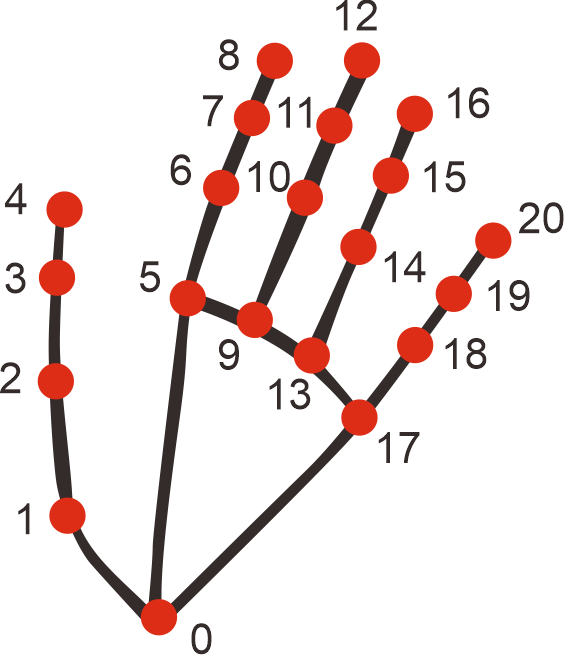
\includegraphics[scale=1]{gambar/mediapipe_hand_landmark.png}
  \caption{Hand Landmarks}
  \label{fig:handlandmarks}
\end{figure}

Dalam proses deteksi pose tangan ini, penulis menggunakan bantuan dari \emph{\emph{library} MediaPipe}. MediaPipe adalah kerangka kerja yang memungkinkan untuk membuat \emph{landmark}, atau titik-titik kunci di berbagai bagian tubuh. Semua titik koordinat dinormalisasi tiga dimensi. MediaPipe menggunakan model \emph{landmark} pose, wajah dan tangan, namun yang digunakan pada penelitian ini hanyalah pada bagian tangan yang dimana terdapat 21 \emph{landmark} dalam tiap \emph{frame} seperti yang ditunjukan pada gambar \ref{fig:handlandmarks}. Dengan menggunakan \emph{\emph{library}} ini dapat langsung menghasilkan prediksi koordinat. Tiap \emph{landmark} yang ada memiliki koordinat x, y, dan z. Dimana untuk nilai x dan y dinormalisasi menjadi lebar dan tinggi dari gambar input yang diterima. Sedangkan z merepresentasikan nilai kedalaman \emph{landmark}, yang nilainya semakin kecil apabila tangan semakin mendekati kamera \parencite{Indriani2021}.

\begin{longtable}{|c|c|}
  \caption{Keterangan Nama Setiap Titik \emph{Landmark}}
  \label{tb:keterangansetiaptitiklandmark}\\
  \hline
  \textbf{Nomor titik} & \textbf{Keterangan} \\
  \hline
  \endhead
  0   & Pergelangan tangan  \\
  1   & Karpal Jempol   \\
  2   & Metakarpal Jempol   \\
  3   & Inter Falang Jempol  \\
  4   & Tuberocity Jempol  \\
  5   & Metakarpal Telunjuk  \\
  6   & Proksimal Palang Telunjuk  \\
  7   & Distal Palang Telunjuk  \\
  8   & Tuberocity Telunjuk  \\
  9   & Metakarpal Jari Tengah  \\
  10  & Proksimal Palang Jari Tengah  \\
  11  & Distal Palang Jari Tengah  \\
  12  & Tuberocity Jari Tengah  \\
  13  & Metakarpal Jari Manis  \\
  14  & Proksimal Palang Jari Manis  \\
  15  & Distal Palang Jari Manis  \\
  16  & Tuberocity Jari Manis  \\
  17  & Metakarpal Kelingking  \\
  18  & Proksimal Palang Kelingking  \\
  19  & Distal Palang Kelingking  \\
  20  & Tuberocity Kelingking  \\
  \hline
\end{longtable}

\subsection{Kontrol \emph{Microsoft Power Point}}
\emph{Microsoft Office PowerPoint} merupakan sebuah aplikasi komputer untuk presentasi yang dikembangkan oleh \emph{\emph{Microsoft}} di dalam paket aplikasi kantoran mereka yaitu \emph{Microsoft Office} \parencite{Poerwanti2018}. \emph{PowerPoint} pada awalnya dirancang untuk menyediakan visual untuk presentasi kelompok dalam organisasi bisnis. Namun, kemudian berkembang pesat ke sektor lainnya, baik dalam bisnis maupun di luarnya. Didalamnya terdapat berbagai fitur yang menunjang presentasi seperti navigasi berpindah slide, \emph{pen tool} untuk mencoret-coret slide beserta \emph{erase} untuk dapat menghapusnya. \emph{Pointer} untuk melakukan \emph{highlight} pada bagian tertentu. Hingga fitur \emph{zoom} untuk memperbesar bagian visual tertentu pada presentasi.

Fitur-fitur tersebut, dapat diakses salah satunya dengan menggunakan \emph{library} bernama \emph{pywin32}. \emph{Pywin32} adalah \emph{library} ekstensi \emph{python} untuk Windows yang memungkinkan menggunakan fitur \emph{Aplication Programming Interface (API) Win32} di\emph{python}. Melalui \emph{library} ini, penggunaan fitur dalam \emph{PowerPoint} bisa diakses melalui property ataupun method yang ada dalam object yang diinginkan. Tersedia juga dokumentasi untuk Object apa saja beserta property dan method nya yang dapat diakses. Selain menggunakan \emph{library} ini, terdapat cara lain yaitu menggunakan \emph{library} yang berfungsi untuk menjalankan fungsi-fungsi yang ada pada \emph{\emph{keyboard}}. Dikarenakan adanya keuntungan dalam menggunakan \emph{PowerPoint} dimana tersedia opsi untuk mengakses fitur-fitur yang ada menggunakan shortcut tertentu pada \emph{keyboard}, maka dapat digunakan \emph{library} bernama \emph{pyautogui}. Dengan menggunakan kedua cara tersebut, membuat proses menghubungkan program \emph{python} yang dibuat bisa terhubung dengan aplikasi \emph{Microsoft} \emph{PowerPoint}.  

% MediaPipe dirancang untuk praktisi pembelajaran mesin (ML), termasuk peneliti, mahasiswa, dan pengembang perangkat lunak, yang mengimplementasikan aplikasi ML siap produksi,
% menerbitkan kode yang menyertai pekerjaan penelitian, dan membangun prototipe teknologi. Kasus penggunaan utama untuk MediaPipe adalah pembuatan prototipe cepat dari saluran persepsi dengan inferensi model dan komponen dapat digunakan kembali lainnya. MediaPipe juga memfasilitasi penerapan teknologi persepsi ke dalam deGambar 1: Deteksi objek menggunakan MediaPipe. Kotak transparan mewakili simpul perhitungan (kalkulator) dalam grafik MediaPipe, kotak padat mewakili input/output eksternal ke grafik, dan garis yang memasuki bagian atas dan keluar dari bagian bawah node masing-masing mewakili aliran input dan output. Port di sebelah kiri beberapa node menunjukkan paket sisi input. Lihat Bagian 6.1 untuk detailnya. mos dan aplikasi pada berbagai platform perangkat keras yang berbeda. MediaPipe memungkinkan peningkatan bertahap pada pipa persepsi melalui konfigurasinya yang kaya bahasa dan alat evaluasi.

% Memodifikasi aplikasi persepsi untuk memasukkan langkah-langkah pemrosesan tambahan atau model inferensi bisa jadi sulit, karena kopling yang berlebihan antara langkah-langkah. Selain itu, mengembangkan aplikasi yang sama untuk platform yang berbeda membutuhkan waktu mengkonsumsi dan biasanya melibatkan pengoptimalan inferensi dan memproses langkah-langkah agar berjalan dengan benar dan efisien pada target perangkat.

% MediaPipe mengatasi tantangan ini dengan mengabstraksi dan
% menghubungkan model persepsi individu menjadi dapat dipertahankan jalur pipa. Semua langkah yang diperlukan untuk menyimpulkan dari data sensorik dan mendapatkan hasil yang dirasakan ditentukan dalam konfigurasi pipa. Sangat mudah untuk menggunakan kembali komponen MediaPipe di pipeline yang berbeda di seluruh aplikasi yang berurutan karena komponen ini memiliki orientasi antarmuka yang sama sekitar data deret waktu. Setiap pipa kemudian dapat dijalankan dengan perilaku yang sama pada berbagai platform, memungkinkan praktisi untuk mengembangkan aplikasi pada workstation, dan lalu terapkan di seluler, misalnya. MediaPipe terdiri dari tiga bagian utama: (a) kerangka kerja untuk inferensi dari data sensorik, (b) seperangkat alat untuk evaluasi kinerja, dan (c) kumpulan inferensi yang dapat digunakan kembali dan komponen pemrosesan yang disebut kalkulator. Kami menjelaskan kerangka kerja di Bagian 3 dan 4, dan seperangkat alat di Bagian 5 Kami juga menyajikan contoh persepsi MediaPipe aplikasi di Bagian 6 \parencite{CamilloLugaresi}. 

\subsection{Convolutional Neural Network}

\begin{figure} [ht] \centering  
  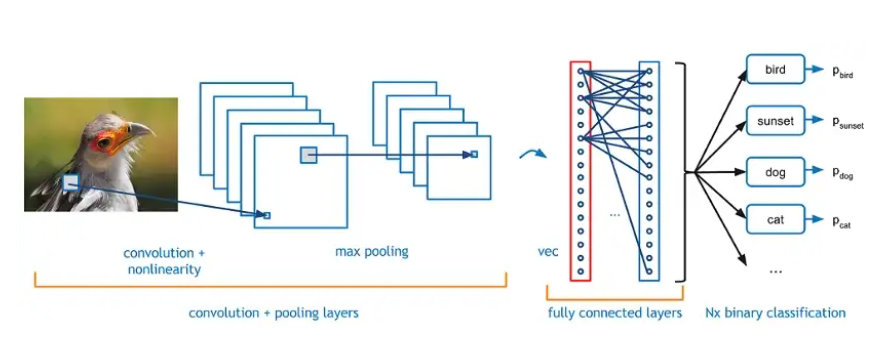
\includegraphics[scale=0.75]{gambar/teori-dasar-cnn.png}
  \caption{Convolutional Neural Networks}
  \label{fig:convolutionalneuralnetworks}
  \parencite{CNN}
\end{figure}

CNN adalah pengembangan dari \emph{Multilayer Perceptron (MLP)} yang didesain untuk mengolah data dua dimensi. Didalamnya terdapat input layer, hidden layer, serta output layer. Dimana didalam layer-layer tersebut berisi banyak kumpulan neuron. MLP sendiri menerima input data yang sifatnya satu dimensi dan mempropagasikan data tersebut pada jaringan hingga menghasilkan output. Tiap hubungan antar neuron pada layer yang bersebelahan memiliki parameter bobot tertentu. Disetiap data input pada layer dilakukan operasi linear dengan nilai bobot yang ada, kemudian hasil komputasi ditransformasi menggunakan operasi yang disebut sebagai fungsi aktivasi. 

Sedangkan pada CNN, data yang dipropagasikan pada jaringan adalah data dua dimensi. Pada CNN operasi linear menggunakan operasi konvolusi, sedangkan bobot tidak lagi satu dimensi saja, namun berbentuk empat dimensi yang merupakan kumpulan kernel konvolusi. Karena sifat proses konvolusi, maka CNN hanya dapat digunakan pada data yang memiliki struktur dua dimensi seperti citra \parencite{IWayan2016}. Belum ada panduan yang betul-betul solid dalam menentukan jumlah \emph{hidden layer} pada sebuah arsitektur model CNN \parencite{MBernico}. Dalam \emph{hidden layer} CNN sendiri, terdapat tiga jenis lapisan utama yaitu :

\begin{enumerate}[nolistsep]
  \item Convolution Layer
  \item Pooling Layer
  \item Fully-connected Layer
\end{enumerate}

\subsubsection{Convolution Layer}
Pada bagian layer ini, sebagian besar komputasi terjadi. Hal ini terjadi karena citra input diproses dengan operasi konvolusi dalam rangka menghasilkan filter citra yang berbeda-beda. Ada tiga komponen penting dalam layer ini, yaitu input data, \emph{filter/kernel}, dan \emph{feature map}. Sebagai contoh, Input data yang diberikan dapat memiliki tiga dimensi. Tiga dimensi ini adalah lebar, tinggi, dan kanal. Perlu diketahui juga, bahwa pendekatan deep learning yang digunakan CNN merupakan supervised learning. Supervised learning adalah teknik pembelajaran menggunakan input dataset yang berlabel \parencite{MdZahangir}. Kemudian, untuk \emph{filter/kernel} memiliki tugas untuk bergerak melintasi citra dan melakukan operasi "dot" antara input citra dengan matriks dari filter. Hasil operasi ini adalah output yang biasa disebut dengan \emph{feature map}. Keseluruhan proses inilah yang dikenal dengan istilah konvolusi. Ilustrasi proses operasi konvolusi ini dapat dilihat pada gambar \ref{fig:Ilustrasi Operasi Konvolusi}.

\begin{figure} [ht] \centering  
  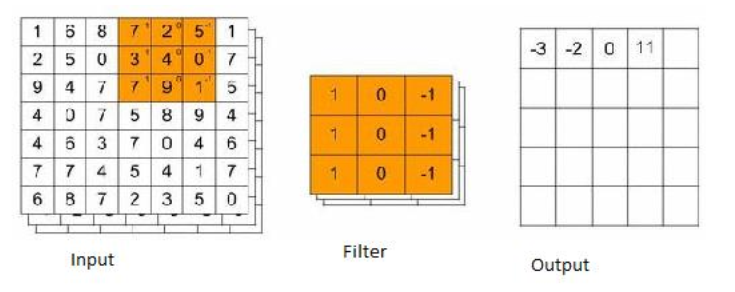
\includegraphics[scale=0.9]{gambar/convolution-operation.png}
  \caption{Ilustrasi Operasi Konvolusi}
  \label{fig:Ilustrasi Operasi Konvolusi}
  \parencite{MaxPoolingLayer}
\end{figure}

Pada Gambar \ref{fig:Ilustrasi Operasi Konvolusi} dapat diketahui bahwa filter bisa berjumlah banyak dan memiliki bentuk berupa matriks. Nilai pada filter tersebut adalah \emph{weight} yang dapat diperbarui nilainya saat proses pelatihan. Dalam layer ini terdapat \emph{hyperparameter} yang bisa diatur. Berikut beberapa diantaranya :

\begin{enumerate}[nolistsep]
  \item Jumlah filter. Banyaknya filter yang digunakan berpengaruh terhadap banyaknya kanal pada \emph{feature map}. Jadi, jika terdapat dua filter yang berbeda misalnya, maka \emph{feature map} yang dihasilkan juga dua dengan nilai yang berbeda.
  \item \emph{Stride}. \emph{Stride} merupakan besarnya jarak perpindahan yang dilalui filter saat melintasi citra saat proses konvolusi. Hal ini mengakibatkan apabila semakin besar nilai \emph{stride}, maka ukuran output yang dihasilkan semakin kecil. 
  \item \emph{Padding}. \emph{Padding} adalah bagian yang ditambahkan pada elemen terluar citra. Umumnya, nilai yang ditambahkan adalah 0 dengan ukuran yanng berbeda-beda. Terdapat tiga jenis \emph{padding} yaitu \emph{valid padding, same padding, dan full padding}. 
\end{enumerate}   

\subsubsection{\emph{Pooling Layer}}
\emph{Pooling layer} adalah bagian layer yang memiliki fungsi untuk \emph{downsampling}. \emph{Downsampling} adalah pengurangan ukuran dimensi dan jumlah parameter. Hal ini dilakukan dengan tujuan mengurangi tingkat kompleksitas untuk layer selanjutnya karena proses ini membuat resolusi dari nilai matriks suatu citra menjadi lebih berkurang. Selain itu, \emph{pooling layer} juga berfungsi untuk mengekstraksi fitur dominan. Umumnya, Ada dua jenis \emph{pooling} yang dapat digunakan yaitu \emph{max pooling} dan \emph{average pooling}. \emph{Max pooling} mengambil nilai maksimum dari citra yang ada dalam suatu kernel. \emph{Average pooling} mengambil nilai rata-rata dari citra yang dalam suatu kernel. 

Sebagai contoh, untuk \emph{max pooling} dapat dilihat dalam gambar \ref{fig:Ilustrasi Max Pooling Layer}. Pada matriks tersebut, ukurannya dibagi tiap kotak 2x2. Tiap bagian kotak tersebut, dicari nilai paling besarnya dan dijadikan output dari nilai matriks yang baru. Begitu juga dengan \emph{average pooling}, prosesnya mirip namun yang membedakan hanya pada nilai yang diambil dari bagian matriks yang dipotongnya. Output nilai matriks yang baru dalam \emph{average pooling} didapatkan dari hasil rata-rata dalam kotak matriks yang dibagi. 

\begin{figure} [ht] \centering  
  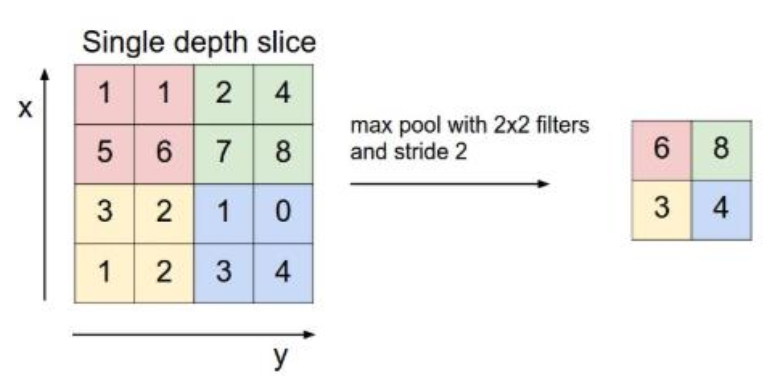
\includegraphics[scale=0.75]{gambar/max-pooling-layer.png}
  \caption{Ilustrasi Max Pooling Layer}
  \label{fig:Ilustrasi Max Pooling Layer}
  \parencite{MaxPoolingLayer}
\end{figure}

\subsubsection{Fully Connected Layer}
Hasil \emph{feature map} dari convolution dan pooling layer memiliki bentuk multidimensional array. Bentuk ini perlu dilakukan reshape menjadi sebuah vektor. Tujuannya, agar dapat menjadi input dari \emph{fully connected layer}. Dalam layer ini menerapkan activation function. Dalam melakukan klasifikasi, activation function yang digunakan biasanya adalah softmax. Hasil akhir dari softmax merupakan nilai probabilitas dengan rentang dari 0 sampai 1. 

\subsection{\emph{Confussion Matrix}}

\begin{figure} [ht] \centering  
  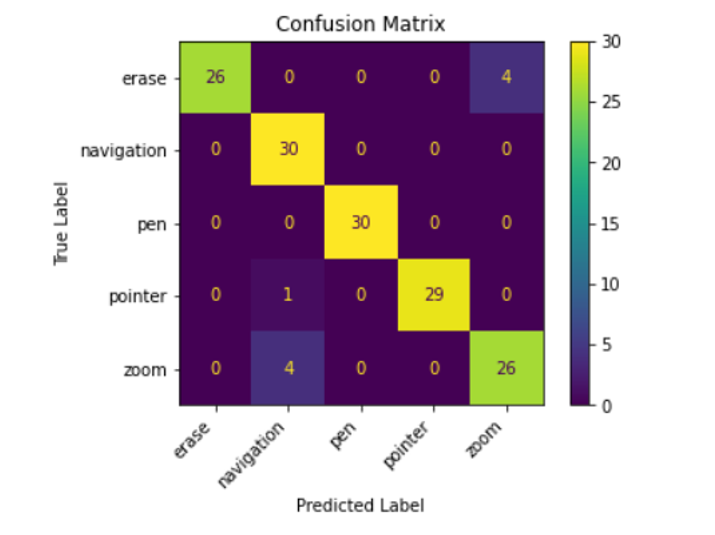
\includegraphics[scale=0.6]{gambar/confussion-matrix.png}
  \caption{Ilustrasi Confusion Matrix}
  \label{fig:Ilustrasi Confusion Matrix}
\end{figure}

Confusion matrix adalah parameter yang digunakan untuk mengukur kinerja model klasifikasi. Salah satu fungsi utama dari confusion matrix adalah untuk mengetahui distribusi atau persebaran hasil klasifikasi kelas mana yang benar atau salah. Confusion matrix dapat diterapkan untuk klasifikasi biner dan klasifikasi multi-class. Gambaran dari bentuk \emph{confusion matrix} sendiri dapat dilihat pada Gambar \ref{fig:Ilustrasi Confusion Matrix}. Terdapat beberapa istilah dalam Confusion matrix yaitu TP, TN, FP, dan FN. berikut adalah penjelasan tiap istilah tersebut \parencite{MohammadReza}.

\begin{enumerate}[nolistsep]
  \item True Positive (TP)
  TP menunjukkan jumlah sampel positif yang diprediksi secara akurat. Contohnya pada klasifikasi suatu gambar. sistem memprediksi bahwa gambar termasuk kelas A dan memang benar gambar tersebut termasuk kelas A.
  \item True Negative (TN)
  TN menunjukkan jumlah sampel negatif yang diprediksi secara akurat. Contohnya pada klasifikasi suatu gambar. sistem memprediksi bahwa gambar tidak termasuk kelas A dan memang benar gambar tersebut tidak termasuk kelas A.
  \item False Positive (FP)
  FP menunjukkan jumlah sampel yang sebenarnya negatif tetapi diprediksi positif. Contohnya pada klasifikasi suatu gambar, sistem memprediksi bahwa gambar termasuk kelas A, namun ternyata gambar tersebut tidak termasuk kelas A. Itu artinya prediksi tersebut salah.
  \item False Negative (FN)
  FN menunjukkan jumlah sampel yang sebenarnya positif tetapi diprediksi negatif. Contohnya pada klasifikasi suatu gambar, sistem memprediksi bahwa gambar tidak termasuk kelas A. namun ternyata gambar tersebut termasuk kelas A. Itu artinya prediksi tersebut salah.
\end{enumerate}   

Representasi dasar confusion matrix juga dapat dilihat pada tabel, dimana istilah TP, TN, FP, dan FN dapat divisualisasikan menjadi data berbentuk tabel.

\begin{longtable}{|c|c|c|}
  \caption{Representasi Dasar \emph{Confusion Matrix}}
  \label{tb:Representasi Dasar Confusion Matrix}\\
  \hline
  \textbf{} & \textbf{Hasil Prediksi 0} & \textbf{Hasil Prediksi 1} \\
  \hline
  Realita 0   &  True Negative    & False Positive  \\
  Realita 1   &  False Negative   & True Positif  \\
  \hline
\end{longtable}

% Kemudian menjadi persamaan seperti pada persamaan \ref{eq:hukumpertamanewton}.

% % Contoh pembuatan persamaan
% \begin{equation}
%   \label{eq:hukumpertamanewton}
%   \sum \mathbf{F} = 0\; \Leftrightarrow\; \frac{\mathrm{d} \mathbf{v} }{\mathrm{d}t} = 0.
% \end{equation}

\cleardoublepage

% Bab 3 desain dan implementasi
\chapter{METODOLOGI}
\label{chap:desainimplementasi}

% Ubah bagian-bagian berikut dengan isi dari desain dan implementasi

Metodologi berisi tentang langkah-langkah yang dilakukan untuk mencapai tujuan dari tugas akhir ini, yang dimana langkah-langkah tersebut digambar dalam blok diagram. Secara umum, gambaran blok diagram metodologi yang digunakan dalam pengerjaan tugas akhir ini adalah sebagai berikut. 

\begin{figure} [ht]
  \centering
  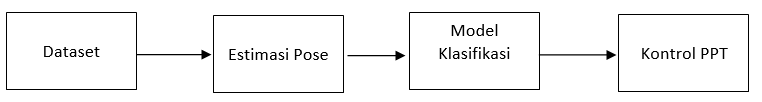
\includegraphics[scale=0.95]{gambar/metodologi.png}
  \caption{Blok Diagram Metodologi}
  \label{fig:Metodologi}
\end{figure}

\section{Dataset}
\label{sec:dataset}

Input citra digunakan sebagai dataset yang nantinya digunakan dalam proses training data. Untuk proses pengambilan dataset dimulai dengan Input citra video. Proses pengambilannya melalui kamera \emph{webcam}, dengan cara mengambil video dan membuatnya menjadi potongan frame-frame. Video yang diambil disesuaikan dengan kelas apa yang ingin diperagakan. Misalnya untuk perintah seperti pengguna \emph{"tool pen"} maka kita harus memperagakan pose \emph{pen} yang telah ditentukan sebelumnya didepan kamera. 

Cara memperagakannya adalah dengan mengambilnya dari beberapa jarak dari dengan kamera. Supaya nantinya deteksi perintah ini dapat terbaca dari berbagai sisi jarak kamera juga. Selain jarak juga dilakukan variasi bentuk pose tangan dan pengambilan angle dibandingkan dengan kamera. Karena, satu orang dalam memeragakan pose tangan tidak selalu sama persis bentuknya dengan yang orang lainnya. 

\begin{longtable}{|c|c|c|}
  \caption{Hasil Pengambilan Dataset}
  \label{tb:Hasil Pengambilan Dataset}\\
  \hline
  \textbf{No.} & \textbf{Kelas Dataset} & \textbf{Citra Dataset} \\
  \hline
  \endhead
  1 & Dataset \emph{Next Slide}  &  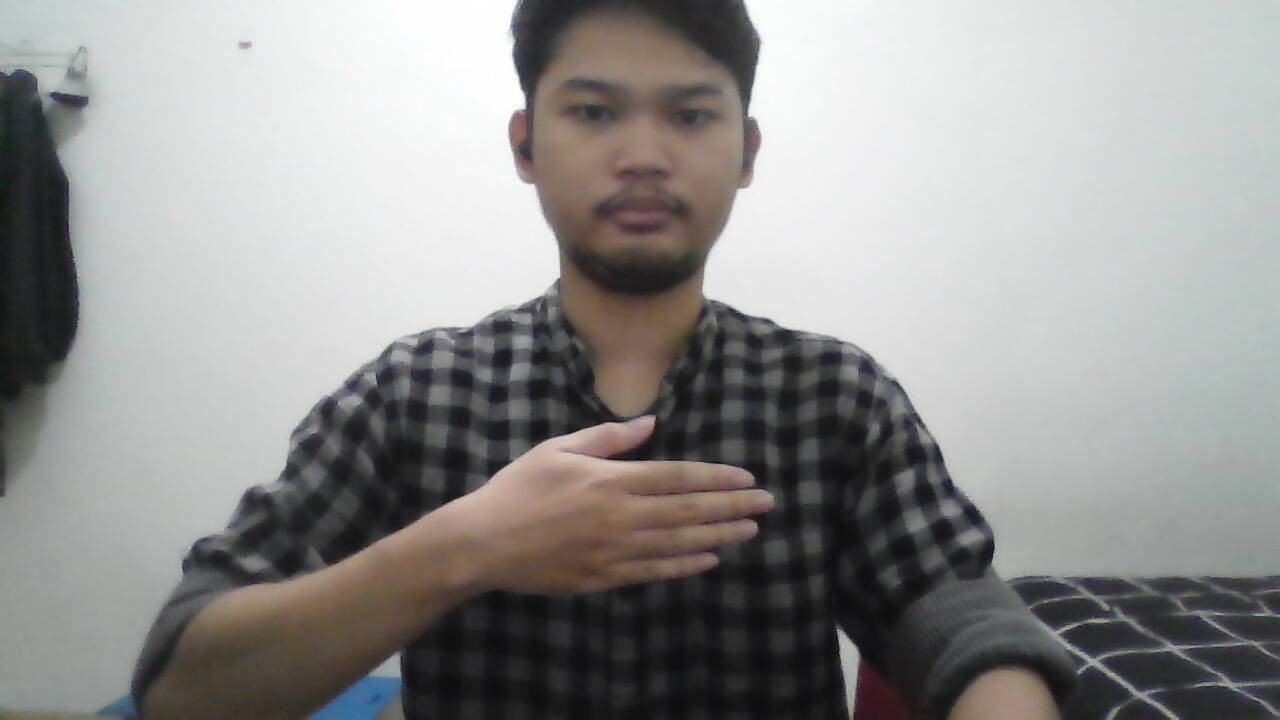
\includegraphics[scale=0.2]{gambar/pengambilan-dataset/dataset-next-slide.jpg} \\
  \hline
  2 & Dataset \emph{Previous Slide}  &  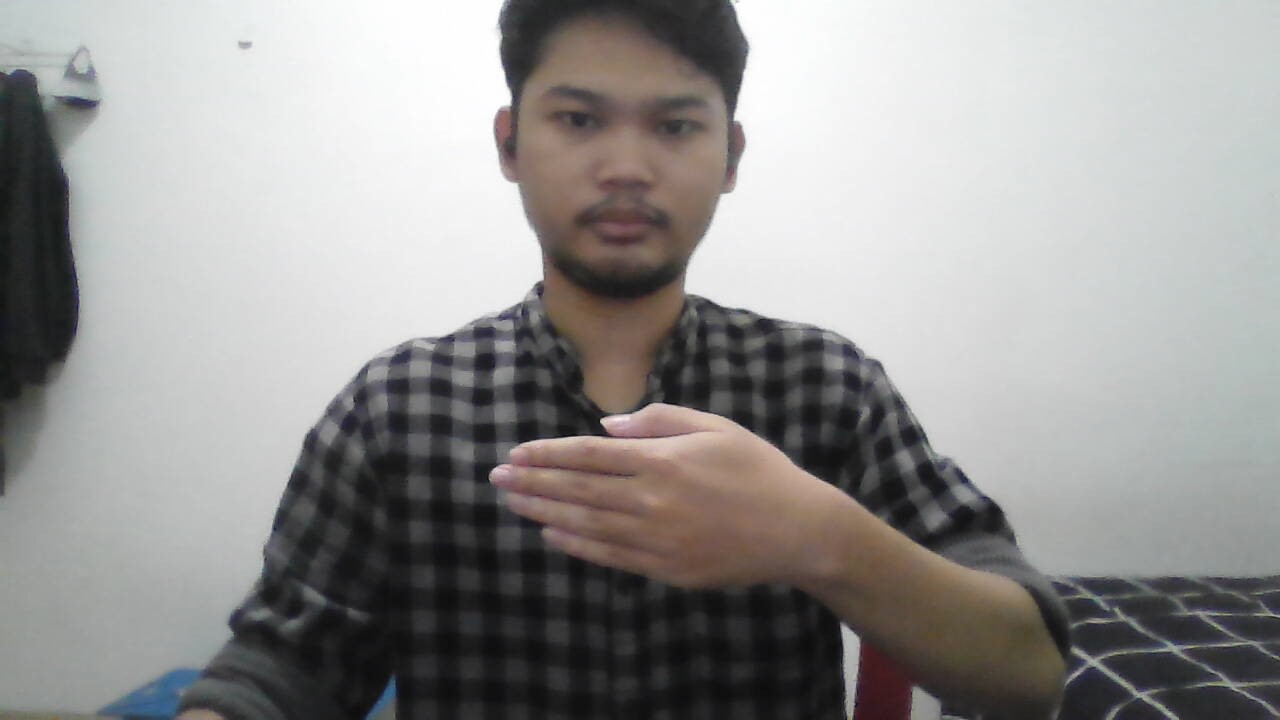
\includegraphics[scale=0.2]{gambar/pengambilan-dataset/dataset-previous-slide.jpg} \\
  \hline
  3 & Dataset \emph{Pointer}  &  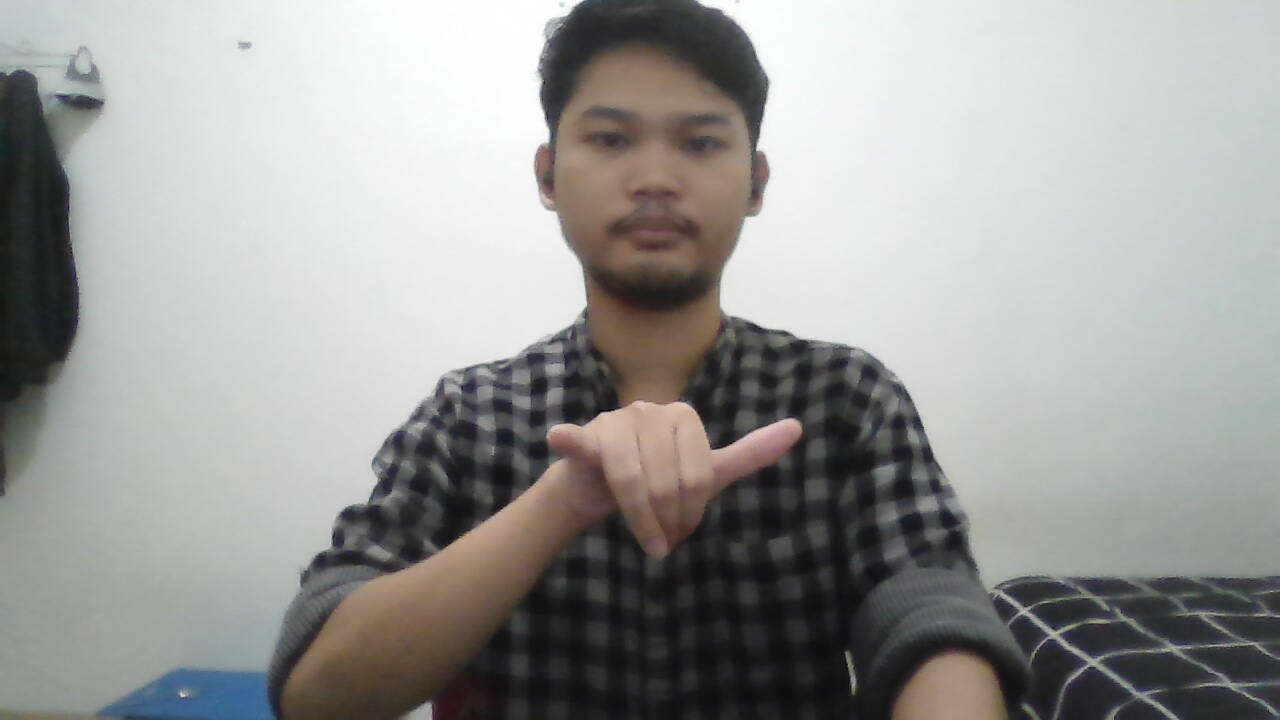
\includegraphics[scale=0.2]{gambar/pengambilan-dataset/dataset-pointer.jpg} \\
  \hline
  4 & Dataset \emph{Zoom Left}  &  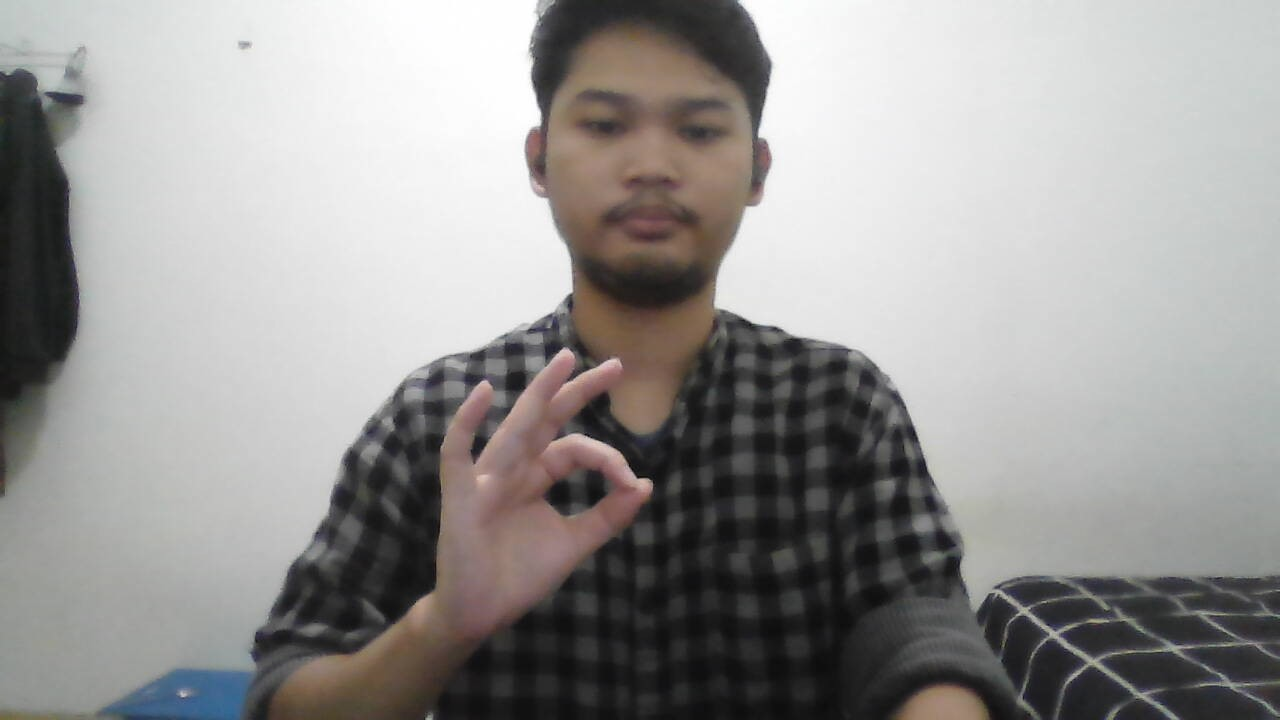
\includegraphics[scale=0.2]{gambar/pengambilan-dataset/dataset-zoom-left.jpg} \\
  \hline
  5 & Dataset \emph{Zoom Right}  &  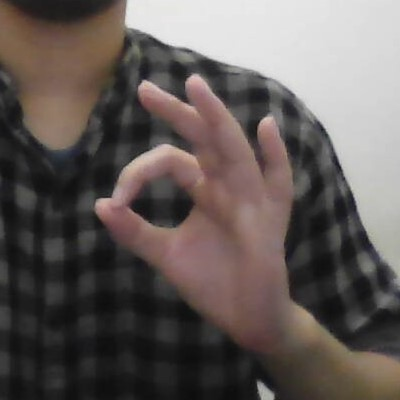
\includegraphics[scale=0.2]{gambar/pengambilan-dataset/dataset-zoom-right.jpg} \\
  \hline
  6 & Dataset \emph{Pen Left}  &  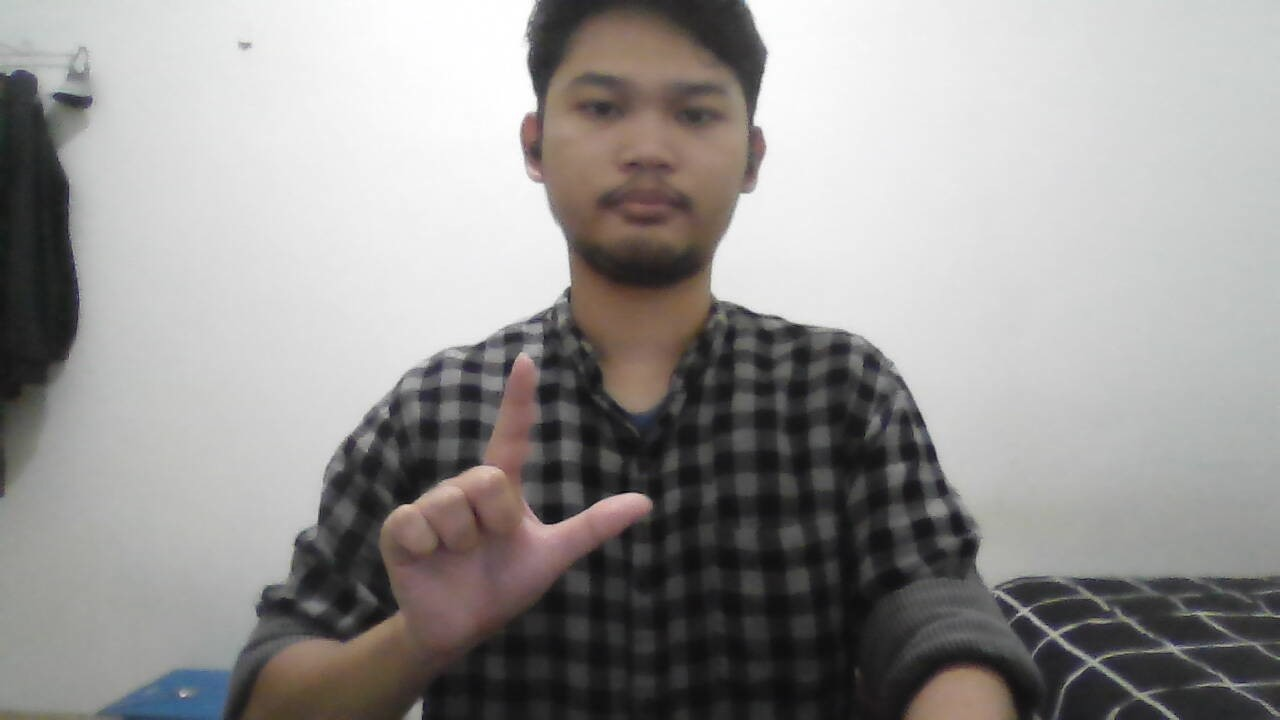
\includegraphics[scale=0.2]{gambar/pengambilan-dataset/dataset-pen-left.jpg} \\
  \hline
  7 & Dataset \emph{Pen Right}  &  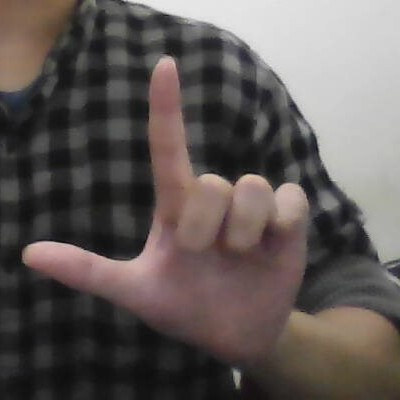
\includegraphics[scale=0.2]{gambar/pengambilan-dataset/dataset-pen-right.jpg} \\
  \hline
  8 & Dataset \emph{Erase}  &  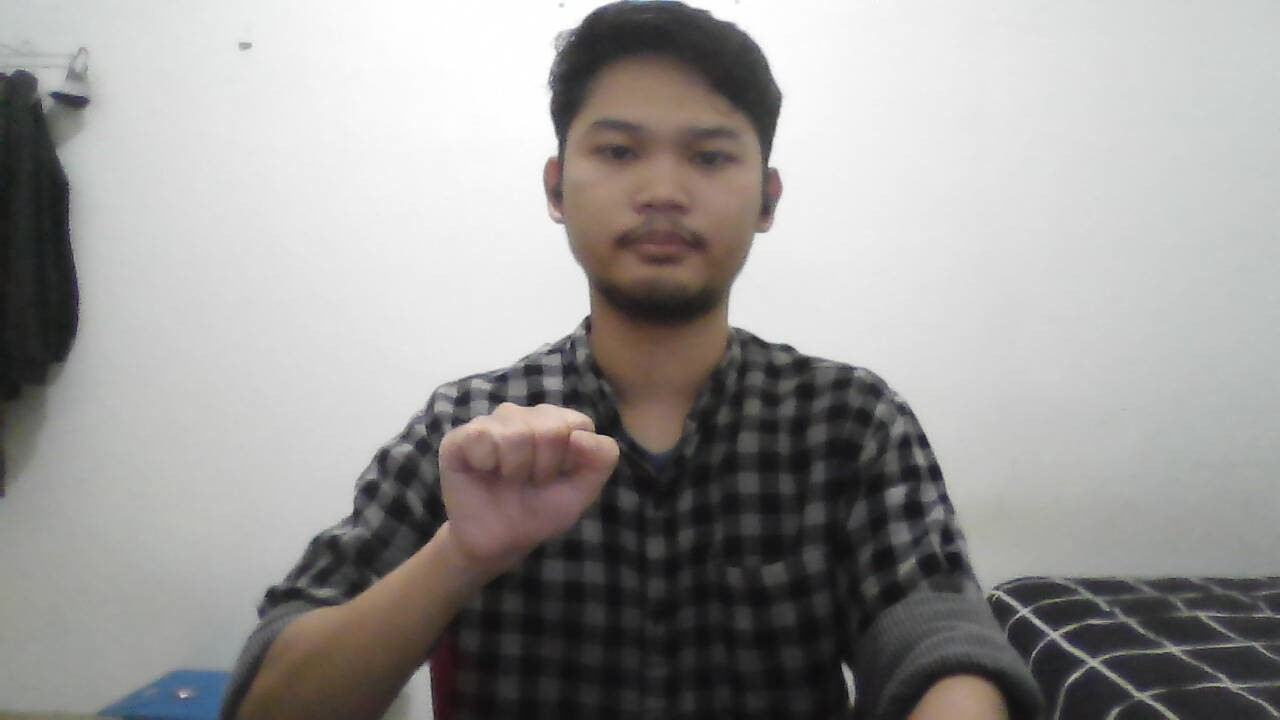
\includegraphics[scale=0.2]{gambar/pengambilan-dataset/dataset-erase.jpg} \\
  \hline
\end{longtable}

Jumlah dan kualitas dari dataset ini juga perlu diperhatikan, karena sangat mempengaruhi kinerja atau hasil tingkat akurasi model yang didapat. Dalam tugas akhir ini banyak citra yang digunakan sebanyak 300 citra pada masing-masing kelas. Karena kelas yang dibuat terdapat delapan kelas, maka total banyaknya citra yang digunakan adalah 2400 citra. Hasil dari pengambilan dataset beserta bentuk pose tangan tiap kelasnya, dapat dilihat dalam Tabel \ref{tb:Hasil Pengambilan Dataset}.

Pada prinsipnya, semakin banyak data akan menambah tingkat akurasi dari sebuah model. Namun, belum ditemukan satu aturan khusus yang pasti mengenai jumlah batas minimal data yang dibutuhkan untuk melatih model dengan tingkat hasil akurasi tertentu. Jumlah data tersebut bergantung pada masalah yang diselesaikan \parencite{Junghwan}. Oleh karenanya, penentuan berapa banyak jumlah data ini perlu dilihat pula hasil akurasinya. Apabila akurasi dirasa cukup maka jumlah dataset tersebut dapat dinyatakan cukup.

Dalam Tabel \ref{tb:Hasil Pengambilan Dataset}, bisa dilihat bahwa pose yang dibuat berjumlah delapan. Padahal banyaknya fungsi yang ingin diterapkan berjumlah enam (\emph{next slide, previous slide, pointer, zoom, pen,} dan \emph{erase}). Hal ini dilakukan karena model yang dibuat, diharapkan dapat mendeteksi tidak hanya menggunakan salah satu tangan saja. Namun, bisa digunakan baik menggunakan tangan kanan maupun tangan kiri. 

Tetapi, tidak semua pose perlu dataset dengan citra dari tangan kanan dan kiri. Karena beberapa pose memiliki kemiripan antara bentuk tangan kanan dan kiri. Dapat dilihat dalam Tabel \ref{tb:Hasil Pengambilan Dataset} bahwa pose untuk fungsi \emph{next slide, previous slide, pointer,} dan \emph{erase} hanya memiliki masing-masing satu kelas. Apabila dilakukan \emph{mirroring} pada citra tersebut hasilnya juga tidak jauh beda. Sehingga, model masih bisa mendeteksi.

Namun, untuk fungsi \emph{pen} dan \emph{zoom} diperlakukan berbeda. Karena bentuk posenya apabila dibandingkan antara menggunakan tangan kanan dengan tangan kiri, terlihat perbedaan yang cukup jauh. Oleh karena itu, cara termudah untuk model dapat mendeteksi tangan kanan maupun kiri dalam pose \emph{pen} dan \emph{zoom} adalah dengan memisahnya menjadi kelas dataset yang terpisah. Hal ini lah yang membuat jumlah kelas dataset terdapat delapan, walaupun jumlah fungsi kontrol \emph{Power Point} yang ingin diterapkan hanya berjumlah enam.

Ukuran frame yang terlihat pada Tabel \ref{tb:Hasil Pengambilan Dataset} sendiri, perlu dipotong supaya hanya citra dari pose tangannya saja yang ditangkap. Namun, proses ini baru bisa dilakukan jika sudah dapat mendeteksi posisi tangan yaitu pada bagian proses estimasi pose. Citra yang digunakan input merupakan citra berwarna yang memiliki tiga buah kanal warna. Tiga buah kanal ini terdiri dari komponen warna RGB yaitu merah/\emph{Red} (R), green/\emph{Green} (G), dan biru/\emph{Biru} (B) yang memiliki nilai dengan rentang mulai dari 0 sampai 255 \parencite{PriyantoHidayatullah}. 

Sebuah dataset perlu dibagi menjadi dua bagian yaitu training set dan validation set. Pembagian ini diperlukan agar dapat mencegah overfitting dan untuk mengevaluasi model. Overfitting yang dimaksud disini adalah kondisi yang terjadi saat model memiliki performa yang sangat baik namun hanya terjadi untuk dataset pelatihan saja. Apabila model diberi data yang belum pernah dilihat sebelumnya, maka performa yang dihasilkan menjadi buruk.

Sebagian besar data dari dataset merupakan Training set. Hal ini karena data pada training set digunakan untuk pelatihan. Apabila proses pelatihan ini selesai, dilakukan proses evaluasi kinerja dari model menggunakan data dari validation set. Jumlah, pembagian banyaknya data pada trainining set dan validation set dalam tugas akhir ini adalah 75\% : 25\%. Proses pengambilan training set dan validation set juga terpisah. Karena model idealnya tidak boleh dilatih menggunakan sample pada validation set, baik sebagian maupun seluruhnya. Sehingga antar training set dan validation set berisi data yang sepenuhnya berbeda. 

\section{Estimasi Pose}
\label{sec:poseprediction}

Estimasi pose memproses frame yang didapat dari hasil pengambilan dataset sebelumnya. Proses ini berguna untuk menentukan \emph{keypoint} untuk membuat kerangka dari pose tangan atau yang disebut \emph{landmark}. Citra tangan dari input kamera yang masih asli, diekstrak menjadi citra yang sudah terdapat kerangka posenya sehingga dapat dianalisa untuk melakukan pengklasifikasian. Dalam proses pendeteksian pose kerangka tangan, penulis menggunakan bantuan sebuah \emph{library} bernama \emph{mediapipe}. \emph{MediaPipe Hands} menggunakan \emph{machine learning} untuk menemukan 21 \emph{landmark} 3D tangan hanya dari satu frame. Tiap frame ini diproses lagi ketahapan selanjutnya bernama ekstraksi fitur. 

Ekstraksi fitur merupakan bagian dari tahapan yang untuk pengenalan pola. Proses ini dilakukan agar dapat memperoleh informasi yang terkandung dalam suatu citra. Jika informasi ini telah didapatkan, maka informasi tersebut digunakan sebagai acuan untuk membedakan antara satu citra dengan citra yang lainnya. Ektraksi fitur ini dapat dilakukan, salah satunya dengan cara memisahkan antara objek dengan \emph{background}. Dalam hal ini, deteksi \emph{landmark} tangan dipisah dari \emph{background} aslinya dan diganti dengan latar berwarna hitam. Sehingga, hanya menyisakan citra berupa \emph{landmark} dari pose tangan saja tanpa ada citra tangan yang asli.   

Hasil dari ekstraksi fitur tersebut, diproses lagi dengan proses \emph{localization}. Proses ini menentukan lokasi objek dengan membuat kotak pembatas pada daerah citra yang terdapat pose tangannya. Kotak pembatas inilah yang menentukan seberapa besar bagian citra yang dipotong. Apabila gambar sudah diganti dengan \emph{background} hitam, selanjutnya gambar dikumpulkan perkelas untuk dijadikan input proses \emph{training}.

Berdasarkan proses \emph{localization} yang dilakuakan, citra dipotong menjadi ukuran frame sebesar 128 x 128 piksel dengan posisi menyesuaikan letak \emph{landmark} tangan. Diberikan juga \emph{padding} sebesar 64 dikiri, atas, kanan, dan bawah citra. Tujuannya agar tidak ada informasi dari ujung-ujung \emph{landmark} yang hilang karena terpotong. Hasilnya seperti yang terlihat pada gambar \ref{tb:Hasil Estimasi Pose}. Hasil dari proses ini kemudian disimpan lagi dalam folder sesuai dengan kelas dari pose yang dilakukan.

\begin{longtable}{|c|c|c|}
  \caption{Hasil Estimasi Pose}
  \label{tb:Hasil Estimasi Pose}\\
  \hline
  \textbf{No.} & \textbf{Kelas Pose} & \textbf{Hasil Citra Estimasi Pose} \\
  \hline
  \endhead
  1 & \emph{Next Slide}  &  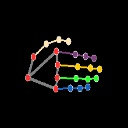
\includegraphics[scale=0.85]{gambar/pose_prediction_next_slide.jpg} \\
  \hline
  2 & \emph{Previous Slide}  &  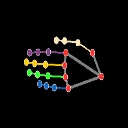
\includegraphics[scale=0.85]{gambar/pose_prediction_previous_slide.jpg} \\
  \hline
  3 & \emph{Pointer}  &  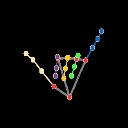
\includegraphics[scale=0.85]{gambar/pose_prediction_pointer.jpg} \\
  \hline
  4 & \emph{Zoom Left}  &  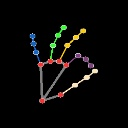
\includegraphics[scale=0.85]{gambar/pose_prediction_zoom_left.jpg} \\
  \hline
  5 & \emph{Zoom Right}  &  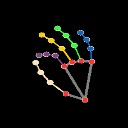
\includegraphics[scale=0.85]{gambar/pose_prediction_zoom_right.jpg} \\
  \hline
  6 & \emph{Pen Left}  &  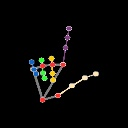
\includegraphics[scale=0.85]{gambar/pose_prediction_pen_left.jpg} \\
  \hline
  7 & \emph{Pen Right}  &  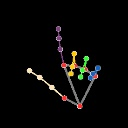
\includegraphics[scale=0.85]{gambar/pose_prediction_pen_right.jpg} \\
  \hline
  8 & \emph{Erase}  &  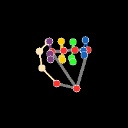
\includegraphics[scale=0.85]{gambar/pose_prediction_erase.jpg} \\
  \hline
\end{longtable}

\section{Model Klasifikasi}
\label{sec:modelklasifikasi}

Tujuan dari pembuatan model adalah dapat menghasilkan model klasifikasi yang dapat memberikan \emph{output} berupa hasil deteksi berdasarkan citra yang diinputkan. Berikut ini proses pembuatan model serta cara memprediksinya. 

\subsection{Pembuatan Model}

Proses pembuatan model dicapai dengan mengatur layer serta \emph{hyperparameter}-nya. Umumnya pengaturan layer ini dibagi menjadi tiga bagian yaitu \emph{convolution layer, pooling layer,} dan \emph{fully connected layer}. Dalam pembuatannya tipe model yang digunakan adalah \emph{Sequential. Sequential} merupakan salah satu cara membuat model dalam \emph{Keras}. Cara ini membuat model dapat dibangun dari satu \emph{layer} ke\emph{layer} lainnya.

Gambaran arsitektur layer model CNN yang digunakan dapat dilihat pada Gambar \ref{fig:cnnlayer}. \emph{Stride} atau jarak perpindahan konvolusi pada semua layer konvolusi sama yaitu satu. Artinya, filter bergeser sebesar satu kotak ukuran matriks pada setiap operasinya. Padding yang digunakan pada semua layer konvolusi dimodel ini juga sama, yaitu valid padding. Valid padding berarti tanpa menggunakan padding sama sekali. Sehingga, output yang dihasilkan (bisa disebut juga dengan \emph{feature map}) berkurang ukurannya masing-masing satu pada kiri, kanan, atas, dan bawah. Jadi, jika ukuran input citranya 128 x 128 maka setelah dikonvolusi hasilnya menjadi 126 x 126. Ukuran filter atau kernelnya yang digunakan tiap konvolusi layer dalam model ini sendiri sama yaitu berukuran 3 x 3. Pada layer pertama jumlah filter yang digunakan sebesar 32. 

\begin{figure} [ht]
  \centering
  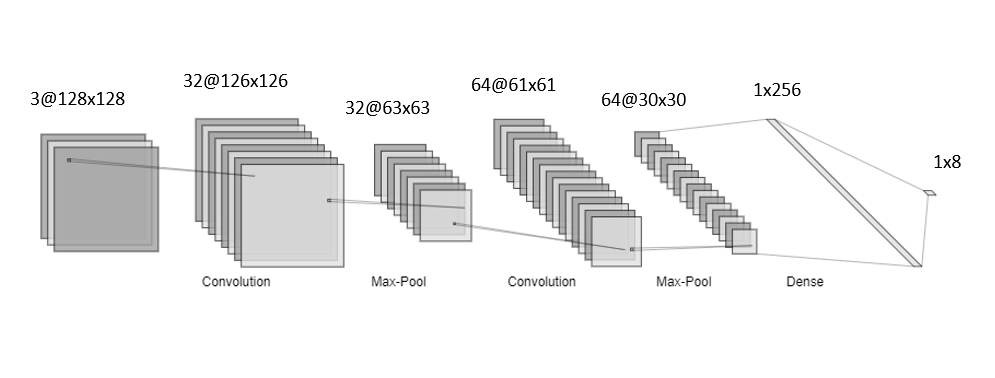
\includegraphics[scale=0.75]{gambar/cnn-layer.png}
  \caption{CNN Layer}
  \label{fig:cnnlayer}
\end{figure}

Pada layer kedua, dilakukan proses \emph{max pooling}. Ukuran max pooling yang digunakan sebesar 2 x 2. Karena ukuran yang digunakan 2 x 2, maka hasil dari pooling layer ini menghasilkan matriks dengan ukuran sebesar setengah dari sebelumnya. Apabila layer yang dilakukan pooling awalnya sebesar 126 x 126, maka hasil setelah dilakukan pooling adalah sebesar 63 x 63.

Dalam layer ketiga, dilakukan proses konvolusi lagi. \emph{Stride}, ukuran filter dan padding yang digunakan sama dengan layer pertama, yang membedakan hanya pada jumlah filternya yang sebesar 64 filter. Layer keempat dilakukan pooling lagi dengan pengaturan sama persis dengan pooling pada layer kedua. Hasilnya berupa feature map berukuran 30 x 30.

Feature map yang dihasilkan dari ekstraksi fitur perlu melakukan flatten karena masih berbentuk multidimensional array. Dari proses tersebut didapatkan sebuah vector. Hal ini bertujuan agar bisa digunakan sebagai input dari fully-connected layer. Lapisan Fully-connected adalah lapisan dimana semua neuron aktivitas dari lapisan sebelumnya terhubung semua dengan neuron di lapisan selanjutnya. Lapisan ini digunakan dengan tujuan untuk mengolah data sehingga bisa diklasifikasikan nantinya. Oleh karena itu, pada Gambar \ref{fig:cnnlayer} bagian paling kanan adalah hasil akhir dimana terdapat array berukuran 1 x 8. Dimana, angka delapan ini menunjukkan jumlah kelas yang ada dalam model ini.

Selain dilakukan pengaturan layer-layer yang digunakan, terdapat hyperparameter yang perlu dikonfigurasi, sebelum melakukan training. Seperti misalnya adalah jumlah epochs, yang digunakan. Epochs sendiri adalah hyperparameter yang memiliki fungsi dalam menentukan banyaknya pengulangan dalam menjalankan algoritma learning dalam proses training. Banyaknya epochs yang digunakan dalam model ini adalah 20 epochs. 

% Proses training ini dimulai dari operasi konvolusi matriks citra, yang kemudian dilanjutkan dengan proses \emph{Max Pooling}. Proses ini dijalankan untuk menghasilkan fitur dari citra yang diinputkan.  

% Terdapat beberapa konfigurasi hyperparameter yang perlu dilakukan terlebih dahulu. Adapun konfigurasi hyperparameter yang dilakukan untuk dataset yang di-train yaitu:

% \begin{enumerate}[nolistsep]
%   \item Epochs. Epochs adalah hyperparameter yang berfungsi untuk menentukan jumlah pengulangan atau berapa kali suatu algoritma learning melakukan proses learning suatu dataset training. Secara sederhana, semakin besar jumlah epochs maka model yang dihasilkan memiliki tingkat akurasi yang lebih tinggi namun waktu yang dibutuhkan untuk melakukan learning akan semakin lambat.
%   \item Batch-Size. Batch-size adalah hyperparameter yang berfungsi untuk mengontrol jumlah sampel training untuk dikerjakan sebelum parameter internal model diperbarui
%   \item Image Size. Image size adalah dimensi ukuran citra yang diterapkan pada dataset. Secara sederhana, semakin kecil dimensi ukurang dari suatu citra maka semakin singkat waktu yang dibutuhkan untuk melakukan proses training.
%   \item Learning Rate. Learning rate adalah hyperparameter yang mengontrol seberapa besar perubahan suatu model dalam menanggapi estimasi kesalahan pada tiap kali weight model diperbarui. Pemilihan nilai learning rate yang tepat diperlukan karena
%   ketika nilai learning rate terlalu kecil maka dapat mengakibatkan proses train yang lama, sedangkan jika nilai learning rate terlalu besar maka dapat mengakibatkan proses learning yang kurang optimal dan terlalu cepat atau proses train yang tidak stabil.
%   \item Optimizer. Optimizer merupakan algoritma atau metode yang digunakan untuk meminimisasi eror (loss function) atau untuk memaksimalkan efisiensi dari produksi. Optimizer merupakan fungsi matematis yang bergantung pada parameter model yang dapat dipelajari seperti weight dan biases. Optimizer sangat membantu untuk mengetahui bagaimana cara mengubah weights ataupun learning rate dari suatu neural network untuk mengurangi nilai loss (Musstafa, 2021). Jenis Optimizer diantaranya yaitu: Adam, Gradient Descent, dan Stochastic Gradient Descent (SGD)
%   (Gupta, 2021).
% \end{enumerate}

\subsection{Prediksi Model}
\label{subsec:Prediksi Model}

Fungsi dari prediksi model klasifikasi ini adalah untuk menyatakan suatu objek kedalam kategori yang sudah ditentukan dengan cara membandingkan input kamera dengan hasil training model mana yang sesuai. Bagian awal dari proses ini adalah deteksi objek tangan yang dimana prosesnya sudah ditangani oleh \emph{framework} mediapipe. Apabila objek tangan terdeteksi, dilanjut dengan proses yang namanya \emph{localization}. \emph{localization} menjadi bagian dari klasifikasi yang menambahkan citra dengan menentukan lokasi objek dengan bantuan \emph{bounding box} atau kotak pembatas. 

Tujuan utama deteksi objek adalah memprediksi lokasi objek dengan \emph{bounding box} atau kotak pembatas dan melakukan klasifikasi objek yang ada pada setiap \emph{bounding box}. Input pada deteksi objek adalah citra yang mengandung satu objek tangan. Sedangkan outputnya adalah hasil prediksi lokasi objek dengan \emph{bounding box} dan klasifikasi kelasnya \parencite{MElgendy}. Ukuran dari kotak ini disamakan dengan dataset yang di-\emph{training}, yaitu 128 x 128. Termasuk juga, didalamnya diberikan padding 64 piksel disemua sisinya seperti yang dilakukan pada Subbab \ref{sec:poseprediction}.

Dalam memprediksi pose yang diinputkan melalui kamera, digunakan sebuah fungsi yang ada pada \emph{library keras}. Output dari fungsi ini adalah array dengan jumlah index sebanyak jumlah kelas yang ada pada model. Sehingga, dari hasil array ini dapat dipilih nilai prediksi yang paling memenuhi untuk klasifikas kelas kita. 

Tampilan secara \emph{real time} hasil prediksi pada program seperti terlihat pada gambar \ref{fig:hasilprediksimodelklasifikasi}. Jika input dari kamera mendeteksi ada pose atau gerakan yang sesuai dengan daftar klasifikasi yang ada, maka proses selanjutnya adalah mengimplementasikan hasil klasifikasi tersebut kedalam aplikasi presentasi yang digunakan.

\begin{figure}[ht]
  \centering
  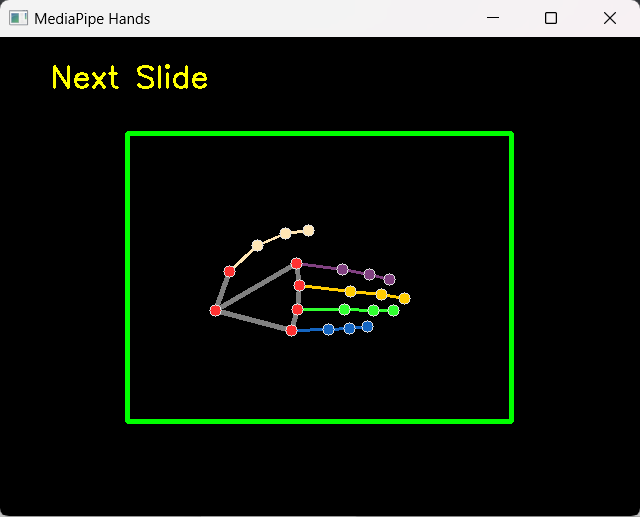
\includegraphics[scale=0.6]{gambar/hasil-prediksi-model-klasifikasi.png}
  \caption{Hasil Prediksi Model Klasifikasi}
  \label{fig:hasilprediksimodelklasifikasi}
\end{figure}

\section{Kontrol PPT}
\label{kontrolppt}

Tahapan ini menghubungkan hasil klasifikasi yang didapatkan dari model, kedalam aplikasi presentasi yang digunakan. Proses implementasi ini membuat program \emph{python} yang dibuat terhubung dengan aplikasi \emph{Microsoft Power Point}. Saat terhubung dilakukan penerapan aksi kontrol kedalam slide presentasi sesuai dengan pose yang terdeteksi.

\subsection{Menghubungkan dengan Fungsi Kontrol PPT}
\label{Menghubungkan dengan Fungsi Kontrol PPT}

Proses ini menggunakan \emph{libray} yang ada pada \emph{python} bernama \emph{pywin32}. Didalamnya terdapat beberapa fungsi yang dapat diakses untuk menavigasi aplikasi \emph{PowerPoint}. Beberapa fungsi dalam aplikasi \emph{Microsoft Power Point} yang dapat diakses adalah seperti navigasi ke slide selanjutnya, navigasi ke slide sebelumnya, dan mengaktifkan \emph{tool pointer}. 

Selain itu, ada cara lain untuk menghubungkan aplikasi \emph{Microsoft Power Point} dengan program yang dibuat yaitu dengan mengakses berbagai macam \emph{shortcut keyboard} yang tersedia. Cara ini dapat dilakukan karena \emph{Microsoft Power Point} memang menyediakan fitur untuk mengontrol presentasi menggunakan keyboard. Sebagai contoh, untuk mengakses fungsi \emph{"pen tool"} dapat menekan tombol \emph{"ctrl"} dan \emph{"p"} secara bersamaan. Daftar lengkap shortcut keyboard untuk kontrol presentasi yang digunakan dalam tugas akhir ini, dapat dilihat pada tabel \ref{tb: daftarshortcutkeyboardmicrosoftpowerpoint}. Perlu diketahui juga, dalam penerapan cara ini dibutuhkan \emph{library pyautogui} supaya dapat mengakses \emph{keyboard} pada perangkat komputer yang digunakan. 

\begin{longtable}{|c|c|}
  \caption{Daftar \emph{Shortcut Keyboard Microsoft Power Point}}
  \label{tb: daftarshortcutkeyboardmicrosoftpowerpoint}\\
  \hline
  \textbf{Perintah Kontrol} & \textbf{Shortcut Keyboard} \\
  \hline
  \emph{erase}   & \emph{'e'}  \\
  \emph{next slide}   & Panah Kanan  \\
  \emph{previous slide}   & Panah Kiri  \\
  \emph{pointer}   & \emph{'ctrl + l'}  \\
  \emph{pen}   & \emph{'ctrl' + 'p'}  \\
  \emph{zoom}   & \emph{'ctrl' + 'mouse wheel up'}  \\
  \hline
\end{longtable}

\subsection{Kontrol Navigasi}
\label{Kontrol Navigasi}
Dalam mengontrol navigasi (\emph{next slide} dan \emph{previous slide}), proses yang dilakukan cukup dengan memanggil fungsi dalam \emph{library pyautogui}. Namun, terdapat satu permasalahan ketika setiap hasil deteksi pose langsung dihubungkan dengan fungsi tersebut. Dimana, aplikasi \emph{Power Point} menjalankan fungsi \emph{next} atau \emph{previous} tersebut secara terus menerus. 

Oleh karena itu, perlu dibuatkan kondisi apabila terdeteksi pose navigasi, maka jalankan fungsi \emph{next} atau \emph{previous} sekali saja. Caranya dengan memberi jeda atau \emph{delay} agar tidak memproses hasil prediksi selanjutnya. Delay yang digunakan adalah sebesar satu detik.

\subsection{Kontrol \emph{Pointer}}
\label{subsec:Kontrol Pointer}

Beberapa perintah tertentu juga perlu menggunakan \emph{cursor} dalam penggunaannya. Salah satunya adalah {tool} untuk \emph{pointer}. Hal ini berarti, dalam penerapannya perlu menghubungkan dengan \emph{library cursor} dan mengubah titik koordinatnya supaya bergerak menyesuaikan gerakan tangan. Oleh karena itu, perlu ditentukan satu titik landmark yang menjadi acuan gerak cursor tersebut. 

Titik landmark yang dipilih adalah titik ke-8, yaitu bagian ujung telunjuk tangan (daftar titik \emph{landmark} dapat dilihat pada Tabel \ref{tb:keterangansetiaptitiklandmark}). Titik ini dipilih karena secara natural dapat menjadi acuan dalam menunjuk sesuatu. Penggunaan ujung telunjuk dapat dirasa lebih memudahkan pengguna untuk menentukan di titik mana pose ingin diarahkan. Penggunaan titik acuan ini juga diterapkan untuk fungsi yang lainnya, yaitu zoom dan pen.

Penghubungan antara input gambar dengan titik koordinat pergerakan \emph{cursor} dilakukan dengan memanfaatkan kemampuan fitur bawaan dari \emph{mediapipe}. Dalam \emph{mediapipe}, dapat diambil data koordinat posisi tangan relatif terhadap ukuran panjang dan lebar kamera. Nilai koordinat yang didapatkan memiliki rentang mulai dari 0 sampai 1. Namun, data ini bersifat \emph{mirror} atau terbalik karena diambil melalui kamera. Jadi, misalnya ukuran kamera yang digunakan adalah 640 x 480. Maka koordinat (0, 0) dalam \emph{mediapipe} berada pada titik piksel (640, 0). Sedangkan untuk koordinat (1, 1), maka letak pikselnya berada pada (0, 480). 

Koordinat yang didapat dari \emph{mediapipe} ini dihubungkan dengan ukuran layar dari komputer, supaya dapat menggerakkan \emph{cursor} pada titik yang diinginkan dalam layar. Cara dalam menghubungkannya melalui operasi perkalian antara rentang koordinat yang didapat dari \emph{mediapipe} dengan ukuran layar. Hasil ini yang menjadi input untuk menentukkan titik \emph{cursor} perlu digerakkan kemana.

Sebagai contoh hasil penerapannya, dapat dilihat pada gambar \ref{fig:Kontrol Pointer}. Dilakukan proses pengaktifan fungsi \emph{pointer} dengan menggunakan hasil klasifikasi pose tangan yang didapatkan dari proses prediksi model yang telah dijelaskan dalam Subbab \ref{subsec:Prediksi Model}.

\begin{figure}[ht]
  \centering
  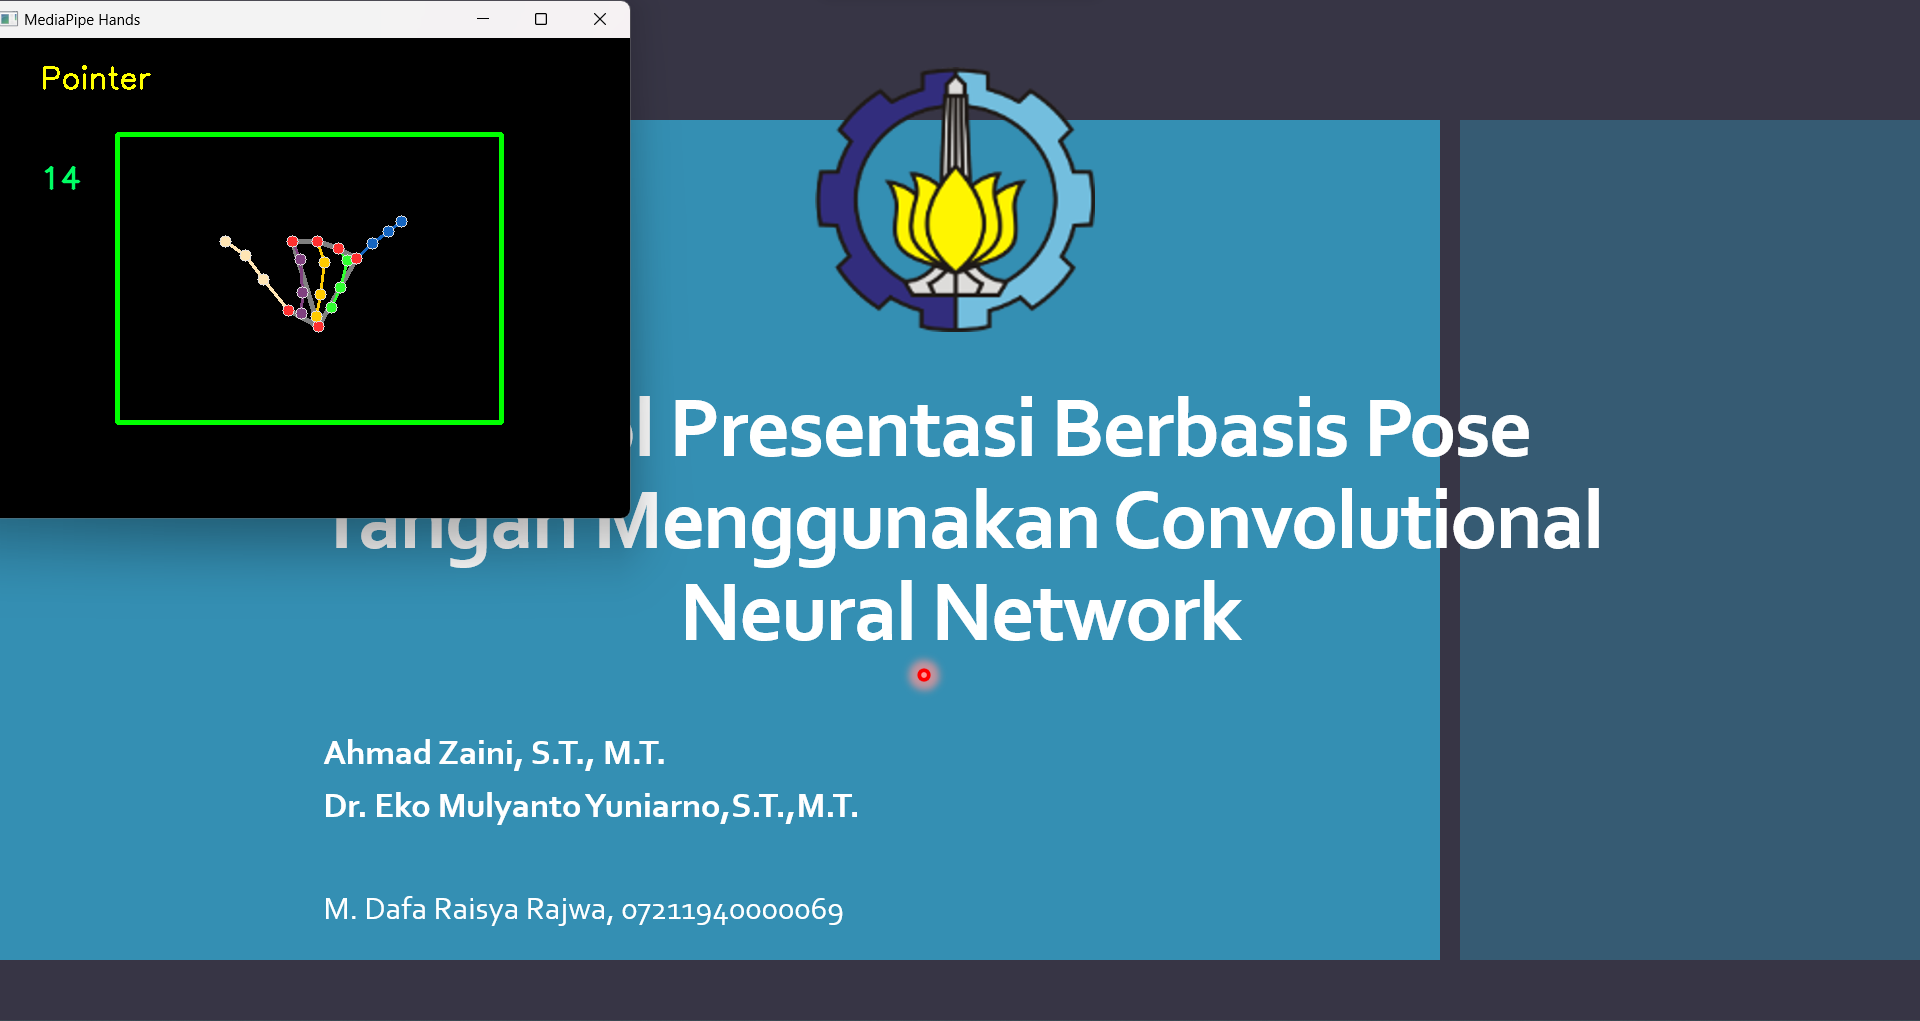
\includegraphics[scale=0.38]{gambar/hasil-kontrol-PPT.png}
  \caption{Kontrol Pointer}
  \label{fig:Kontrol Pointer}
\end{figure}

\subsection{Kontrol \emph{Pen}}
\label{subsec:Kontrol Pen}

Dalam penerapan fungsi \emph{pen} penentuan titik koordinatnya sama persis dengan yang fungsi \emph{pointer} yang dijelaskan pada Subbab \ref{subsec:Kontrol Pointer}. Pembedanya adalah pada kondisi untuk menggambarnya. Pada kontrol ini saat posisi pose \emph{pen} terdeteksi, program dibuat untuk berpindah \emph{state} kedalam mode menggambar.

Perubahan \emph{state} yang dilakukan memiliki tujuan tertentu. Pertama, dapat menghindari perubahan hasil deteksi ketika sedang menggerakkan tangan ketika menggambar. Selain itu, saat berubah \emph{state} proses prediksi model untuk klasifikasi juga tidak dijalankan. Sehingga saat sedang menggambar diharapkan tidak terjadi proses komputasi yang tidak perlu dan bisa menurunkan \emph{frame rate}.

Pada \emph{state pen} ini mengaktifkan fitur \emph{pen} dan menggerakkan \emph{cursor}, namun tidak menekan tombol klik. Penekanan tombol klik baru dilakukan ketika bagian ujung jempol dihubungkan dengan jari tengah. mekanisme tersebut dibuat agar penggunaan fitur \emph{pen} terasa lebih mudah seperti menggunakan \emph{mouse}. Cara kerjanya adalah dengan mengukur jarak antara titik ujung jempol dengan bagian dari jari tengah. Tepatnya pada titik \emph{landmark} ke-10 dan ke-4 (Detail letak titik ini dapat dilihat pada Tabel \ref{tb:keterangansetiaptitiklandmark}). Jika jaraknya diangka lebih kecil dari 0,05 maka program mengirimkan input untuk menekan klik kiri pada \emph{mouse} dan jika tidak maka penekanan klik ini akan dilepaskan.

\subsection{Kontrol \emph{Zoom In}}
\label{subsec:Kontrol Zoom In}

Kontrol zoom pada dasarnya sama dengan pen, yang membedakan pada kondisi \emph{trigger} fungsi zoom. Pada kontrol ini yang menjadi acuan adalah jarak antara ujung jempol dengan ujung telunjuk. Lebih tepatnya titik \emph{landmark} ke-8 dan ke-4. Jika jaraknya masih terhitung menempel maka fungsi zoom belum dijalankan. Namun, jika jaraknya mulai menjauh baru menjalankan fungsi zoom. Besarnya zoom yang dilakukan adalah sebesar 50\%. 

\subsection{Kontrol \emph{Erase}}
\label{subsec:Kontrol Erase}
Kontrol pada \emph{erase} lebih sederhana dibandingkan dengan fungsi-fungsi sebelumnya. Jika hasil prediksi pose menghasilkan kelas \emph{erase}, maka program menjalankan fungsi \emph{erase} melalui \emph{library pyautogui}. Perlu diketahui bahwa fungsi \emph{erase} disini untuk menghapus coretan \emph{pen}. Penghapusan yang dilakukan langsung membersihkan seluruh coretan dalam satu layar sekaligus.
\cleardoublepage

% Bab 4 pengujian dan analisis
\chapter{PENGUJIAN DAN PEMBAHASAN}
\label{chap:pengujiandanpembahasan}

Dalam bab ini dijelaskan mengenai pengujian yang dilakukan berdasarkan hasil pelaksanaan pada bab \ref{chap:desainimplementasi}. Selain itu, juga dibahas dan dianalisa hasil dari pengujiannya. Melalui pengujian dan analisa mengenai hasil penelitian, diharapkan dapat menjadi acuan dalam pengambilan kesimpulan dari pelaksanaan tugas akhir ini.

% \section{Hasil Penelitian}
% \label{sec:hasilpenelitian}

% Hasil penelitian yang dimaksud disini merupakan hasil pelaksanaan dari tiap proses yang sudah dirancang sebelumnya pada tiap blok diagram metodologi dalam Bab \ref{chap:desainimplementasi}. Berikut ini adalah pembahasan mengenai tiap tahapannya.

% \subsection{Hasil Pengambilan Dataset}
% \label{subsec:hasilpengambilandataset}

% \subsection{Hasil Estimasi Pose}
% \label{subsec:hasilposeprediction}

% % \begin{figure}[!htb]
% %   \centering
% %   \begin{subfigure}{0.31\textwidth}
% %     \centering
% %     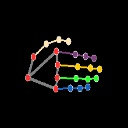
\includegraphics[width=\linewidth]{gambar/pose_prediction_next_slide.jpg}
% %     \caption{next slide}
% %     \label{fig:landmarknextslide} 
% %   \end{subfigure}
% %   \quad
% %   \begin{subfigure}{0.31\textwidth}
% %     \centering
% %     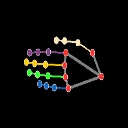
\includegraphics[width=\linewidth]{gambar/pose_prediction_previous_slide.jpg}
% %     \caption{previous slide}
% %     \label{fig:landmarkpreviousslide} 
% %   \end{subfigure}
% %   \quad
% %   \begin{subfigure}{0.31\textwidth}
% %     \centering
% %     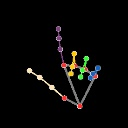
\includegraphics[width=\linewidth]{gambar/pose_prediction_pen_right.jpg}
% %     \caption{pen}
% %     \label{fig:landmarkpen}
% %   \end{subfigure}
% %   \quad
% %   \begin{subfigure}{0.31\textwidth}
% %     \centering
% %     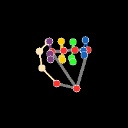
\includegraphics[width=\linewidth]{gambar/pose_prediction_erase.jpg}
% %     \caption{erase}
% %     \label{fig:landmarkerase}
% %   \end{subfigure}
% %   \quad
% %   \begin{subfigure}{0.31\textwidth}
% %     \centering
% %     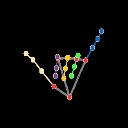
\includegraphics[width=\linewidth]{gambar/pose_prediction_pointer.jpg}
% %     \caption{pointer}
% %     \label{fig:landmarkpointer}
% %   \end{subfigure}
% %   \quad
% %   \begin{subfigure}{0.31\textwidth}
% %     \centering
% %     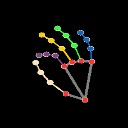
\includegraphics[width=\linewidth]{gambar/pose_prediction_zoom_right.jpg}
% %     \caption{zoom}
% %     \label{fig:landmarkzoom}
% %   \end{subfigure}
% %   \caption{Hasil estimasi pose}
% %   \label{fig:hasilposeprediction}
% % \end{figure}

% \subsection{Hasil Model Klasifikasi}
% \label{subsec:hasilmodelklasifikasi}

% % \begin{longtable}{|c|c|}
% %   \caption{Detail Hyperparameter yang Digunakan}
% %   \label{tb:detailhyperparameteryangdigunakan}\\
% %   \hline
% %   \rowcolor[HTML]{C0C0C0}
% %   \textbf{Weights} & \textbf{CNN} \\
% %   \hline
% %   Class Number            & 6            \\
% %   Epochs                  & 25           \\
% %   Batch-Size              & 16           \\
% %   Image Size              & 128 x 128    \\
% %   Learning rate           & 0.01         \\
% %   Optimizer               & SGD          \\
% %   Jumlah layer konvolusi  & 2            \\
% %   \hline
% % \end{longtable}

% \subsection{Hasil Kontrol PowerPoint}
% \label{subsec:hasilkontrolpowerpoint}

\section{Skenario Pengujian}
\label{sec:skenariopengujian}

Pada tugas akhir ini dilakukan empat skenario pengujian. Pengujian ini diperlukan untuk mengetahui tingkat keberhasilan atau kesalahan agar dapat ditarik kesimpulan yang sesuai. Berikut ini adalah daftar skenario pengujiannya.

\begin{enumerate}[nolistsep]

  \item Pengujian hasil training dan validasi model CNN
  \item Pengujian dengan menggunakan variasi jarak dataset
  \item Pengujian dengan menggunakan variasi Pencahayaan
  \item Pengujian tingkat \emph{Frame Rate}
  \item Pengujian dengan menggunakan tangan dari responden yang berbeda
  \item Pengujian dengan membandingkan model lain (\emph{Resnet50, VGG16,} dan \emph{MobileNet}) 
  \item Pengujian \emph{user experience}

\end{enumerate}

\section{Hasil Pengujian}
\label{sec:hasilpengujian}

Hasil pengujian adalah implementasi dari skenario pengujian yang sudah dijelaskan pada bab 4.2, untuk hasil lengkapnya dapat dilihat pada penjelasan berikut ini.

\subsection{Hasil Pengujian Model}
\label{subsec:hasilpengujianmodel}

\begin{figure}[!htb]
  \centering
  \begin{subfigure}{0.53\textwidth}
    \centering
    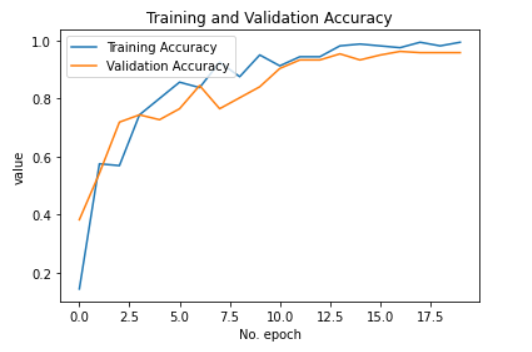
\includegraphics[width=\linewidth]{gambar/training-validation-accuracy.png}
    \caption{Training and Validation Accuracy}
    \label{fig:landmarknextslide} 
  \end{subfigure}
  \begin{subfigure}{0.46\textwidth}
    \centering
    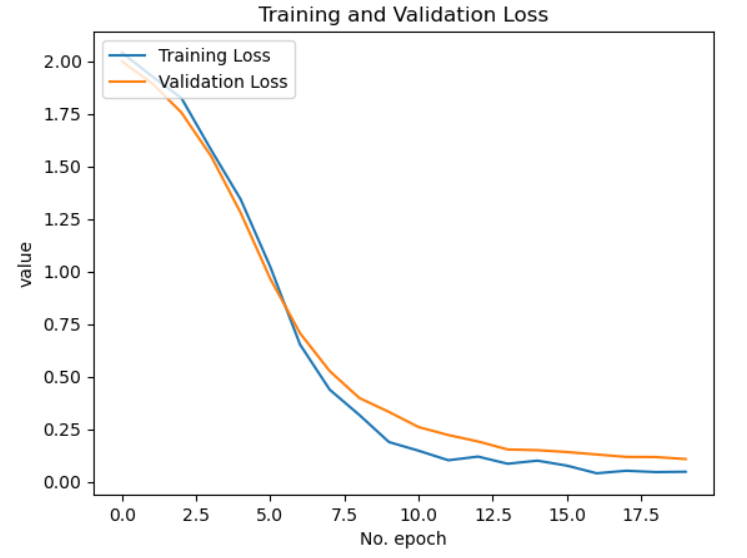
\includegraphics[width=\linewidth]{gambar/training-validation-loss.png}
    \caption{Training and Validation Loss}
    \label{fig:landmarkpreviousslide} 
  \end{subfigure}
  \caption{Hasil Pengujian Model}
  \label{fig:Pengujian Training Validation}
\end{figure}

\hfill \break

Pengujian model bertujuan untuk mengukur akurasi dari model yang dibuat berdasarkan hasil training yang dilakukan menggunakan \emph{library tensorflow}. Akurasi ini dapat diukur dari hasil perhitungan tiap \emph{epoch} yang dilakukan. Grafik pengujian model perbandingan antara akurasi \emph{training} dengan \emph{validation} pada tiap \emph{epoch}, dapat dilihat pada gambar \ref{fig:Pengujian Training Validation}. Training yang dimaksud disini adalah hasil model dari dataset yang dilatih. Sedangkan validation menggunakan dataset yang belum pernah dilihat sebelumnya (berbeda dengan dataset pada training).

Sedangkan untuk perbedaan akurasi dan loss adalah akurasi merupakan banyaknya hasil prediksi yang diklasifikasikan dengan benar. Sedangkan, loss adalah nilai yang menunjukkan perbedaan dari target yang diharapkan. Melalui Grafik \ref{fig:Pengujian Training Validation} didapatkan informasi bahwa nilai akurasi tiap \emph{epoch} menunjukkan adanya peningkatan dari waktu kewaktu. Nilai akurasi \emph{training} akhirnya ada pada 99\%. Sedangkan, untuk akurasi \emph{validation} akhirnya ada pada kisaran 96\%. Performa akurasi model yang hampir sama antara training dan validasi adalah hasil yang baik, karena artinya model dapat memprediksi data yang belum pernah dilihat sebelumnya.

Pada training loss didapatkan nilai dikisaran 0,03. Sedangkan, validation loss dikisaran 0,12. Jarak antara training dan validation dengan nilai loss yang semakin kecil ini menunjukkan prediksi yang error pada model juga kecil.

\subsection{Hasil Pengujian Menggunakan Variasi Jarak}
\label{subsec:Hasil Pengujian Menggunakan Variasi Jarak}

Skenario pengujian menggunakan variasi jarak bertujuan mengukur akurasi dari setiap jarak yang ditentukan. Hal ini dapat menunjukkan seberapa baik kemampuan model dalam mendeteksi klasifikasi pose tangan pada jarak tertentu. Akurasi pengujian model ini diukur dengan membuat data pengujian, dimana data pengujian ini berisi input citra yang diambil diluar dataset. Variasi jarak yang digunakan sendiri dapat dilihat pada Tabel \ref{tb:Gambaran Kondisi Pengujian Jarak} dimana pengujian dilakukan pada jarak 40 cm, 60 cm, 100 cm. Data yang telah didapat dapat dihitung berapa banyak data yang benar sesuai hasil prediksi dan berapa banyak yang tidak sesuai hasil prediksi.

\begin{longtable}{|c|c|c|}
  \caption{Gambaran Kondisi Pengujian Jarak}
  \label{tb:Gambaran Kondisi Pengujian Jarak}\\
  \hline
  \textbf{No.} & \textbf{Jarak (cm)} & \textbf{Gambar Pengujian} \\
  \hline
  \endhead
  1 & \emph{40}  &  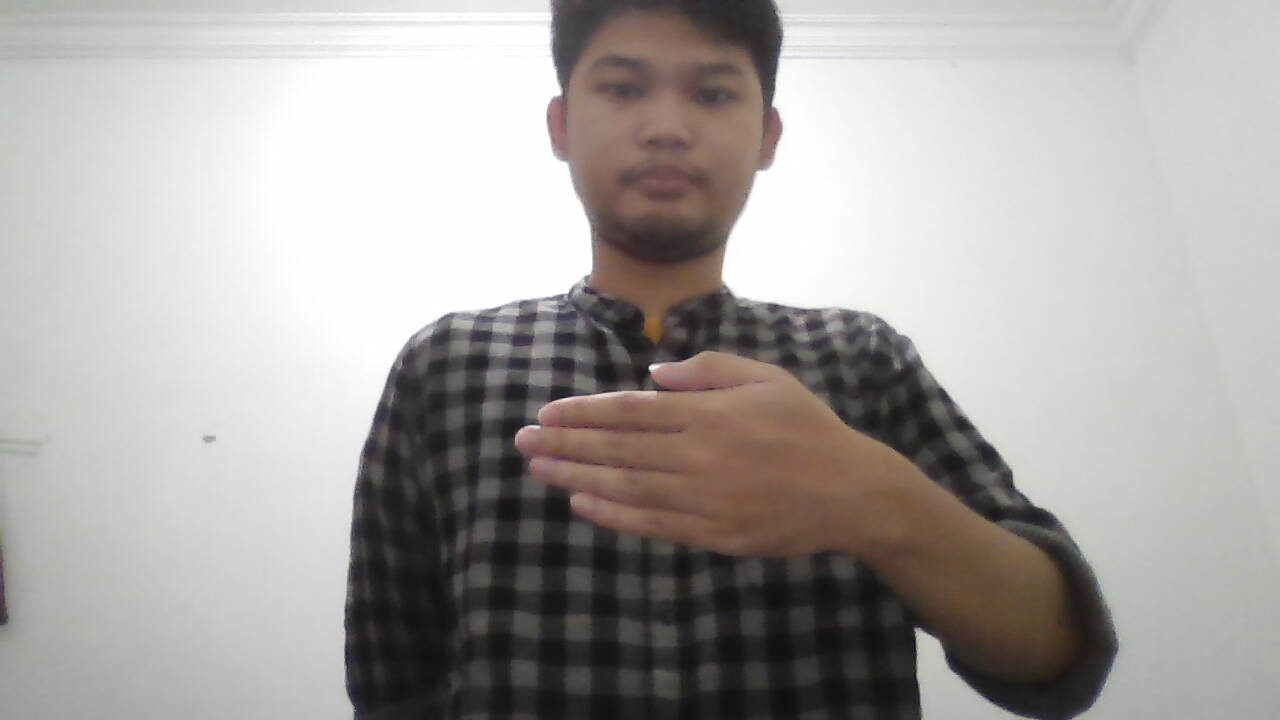
\includegraphics[scale=0.2]{gambar/pengujian-jarak/pengambilan-data/jarak-40cm.jpg} \\
  \hline
  2 & \emph{60}  &  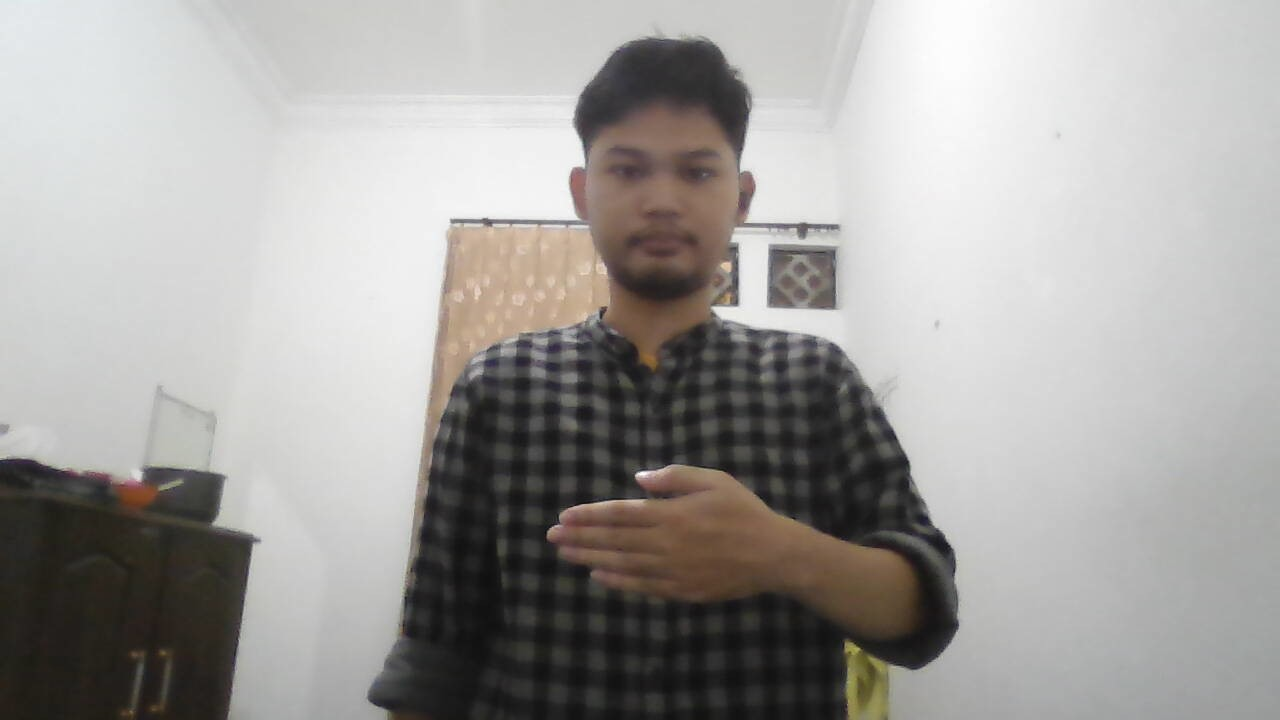
\includegraphics[scale=0.2]{gambar/pengujian-jarak/pengambilan-data/jarak-60cm.jpg} \\
  \hline
  3 & \emph{80}  &  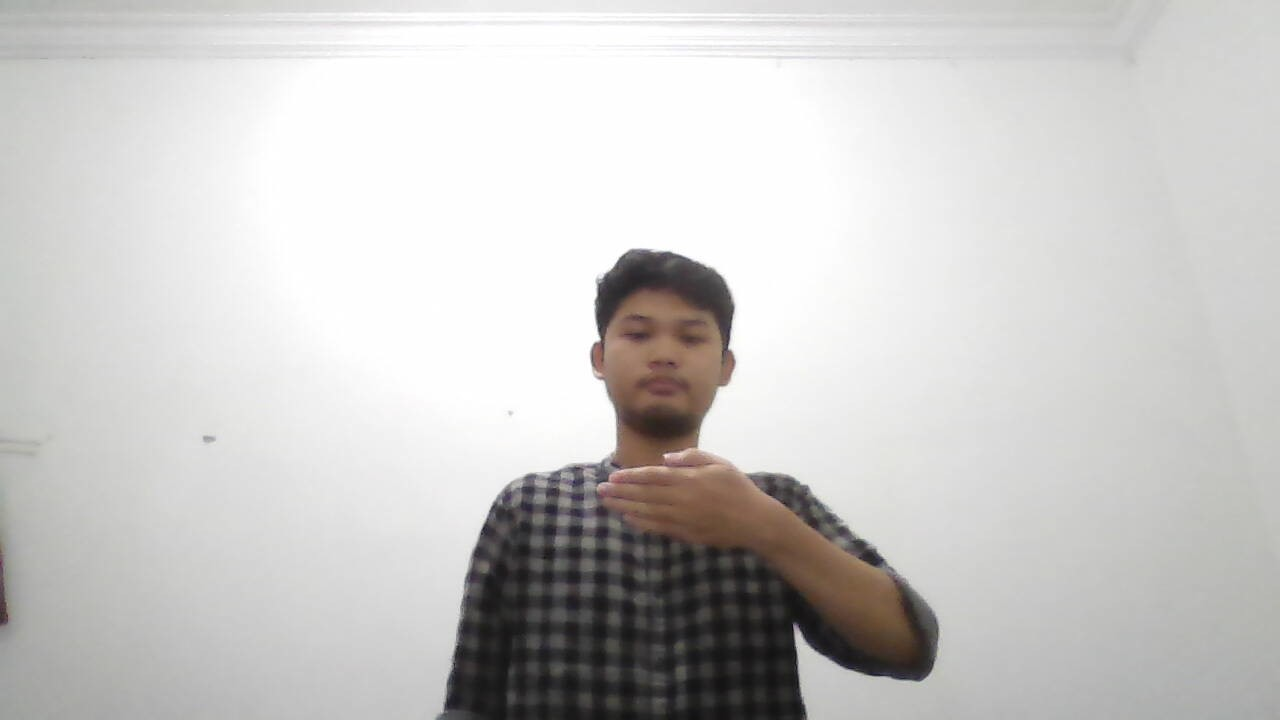
\includegraphics[scale=0.2]{gambar/pengujian-jarak/pengambilan-data/jarak-80cm.jpg} \\
  \hline
  4 & \emph{100}  &  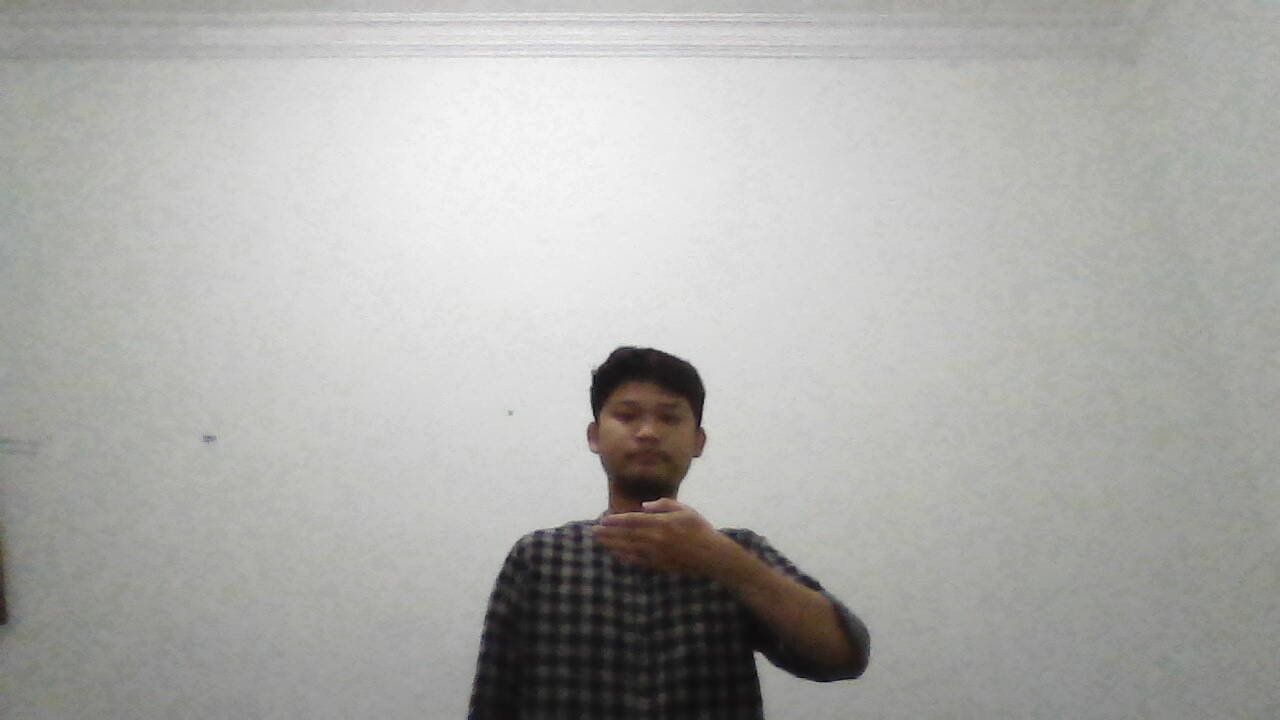
\includegraphics[scale=0.2]{gambar/pengujian-jarak/pengambilan-data/jarak-100cm.jpg} \\
  \hline
\end{longtable}

Pengujian variasi jarak ini diuji dengan menggunakan dua model yang memiliki perbedaan pada datasetnya. Model yang pertama menggunakan kumpulan dataset yang dimana posisi pengambilan datanya bersifat statis disatu jarak tertentu. Jarak yang digunakan dalam model pertama ini adalah sejauh 40 cm. Selain model tersebut, dibuat pula model yang kedua. Model kedua ini menggunakan kumpulan dataset yang posisi pengambilannya bervariasi mulai dari 40 cm hingga 100 cm. Tujuan dilakukannya variasi pengambilan dataset ini untuk diuji apakah model ini dapat mendeteksi lebih baik  dibandingkan dengan model yang hanya menggunakan dataset dengna satu variasi jarak saja. Berikut ini adalah hasil dari pengujian menggunakan variasi jarak.

\subsubsection{Pengujian Menggunakan Dataset Satu Jarak}
\label{subsubsec:Pengujian Menggunakan Dataset Satu Jarak}

Dalam model pertama ini, seperti yang telah disebut dalam bab \ref{subsec:Hasil Pengujian Menggunakan Variasi Jarak} jarak yang digunakan sebagai pengambilan dataset adalah sebesar 40 cm yang berarti ini sama dengan panjang jarak pada variasi yang terdekat. Hasil distribusi prediksi klasifikasi dapat dilihat pada Gambar \ref{fig:Pengujian Tanpa Variasi Jarak Dataset (40 cm)} untuk jarak 40 cm, Gambar \ref{fig:Pengujian Tanpa Variasi Jarak Dataset (60 cm)} untuk jarak 60 cm, Gambar \ref{fig:Pengujian Tanpa Variasi Jarak Dataset (80 cm)} untuk jarak 80 cm, dan Gambar \ref{fig:Pengujian Tanpa Variasi Jarak Dataset (100 cm)}. Hasil distribusinya cukup beragam namun hampir semuanya terdapat kesalahan prediksi yang masuk kedalam kelas \emph{erase}.  

Hasil akurasinya dapat dilihat pada Tabel \ref{tb:Hasil Pengujian Tanpa Variasi Jarak Dataset}. Melalui data tersebut didapatkan hasil bahwa tingkat akurasi yang didapatkan mengalami penurunan setiap jaraknya diperlebar, dimana saat jarak 40 cm didapatkan akurasi sebesar 96.00 \%, saat jarak 60 cm didapatkan akurasi 95.00 \%. Sedangkan saat jarak 80 cm akurasinya sebesar 75.50 \% dan yang terakhir saat jarak 100 cm didapatkan akurasi sebesar 68.00 \%. Berkurangnya akurasi seiring bertambahnya jarak terjadi karena berkurangnya keakuratan titik \emph{landmark} yang dapat dideteksi. Selain itu, bisa diketahui juga bahwa jarak yang paling ideal adalah jarak yang sesuai dengan pengambilan dataset yaitu sebesar 40 cm.

\begin{figure}[!htb]
  \centering
  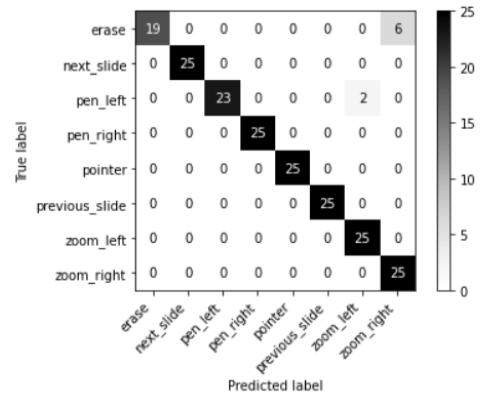
\includegraphics[scale=0.79]{gambar/pengujian-jarak/homogen-dataset/40cm.png}
  \caption{Pengujian Tanpa Variasi Jarak Dataset (40 cm)}
  \label{fig:Pengujian Tanpa Variasi Jarak Dataset (40 cm)}
\end{figure}

\begin{figure}[!htb]
  \centering
  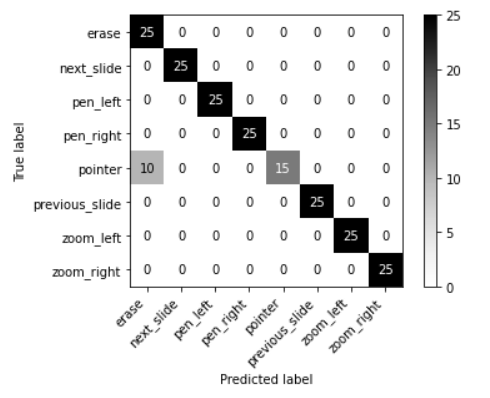
\includegraphics[scale=0.79]{gambar/pengujian-jarak/homogen-dataset/60cm.png}
  \caption{Pengujian Tanpa Variasi Jarak Dataset (60 cm)}
  \label{fig:Pengujian Tanpa Variasi Jarak Dataset (60 cm)}
\end{figure}

\begin{figure}[!htb]
  \centering
  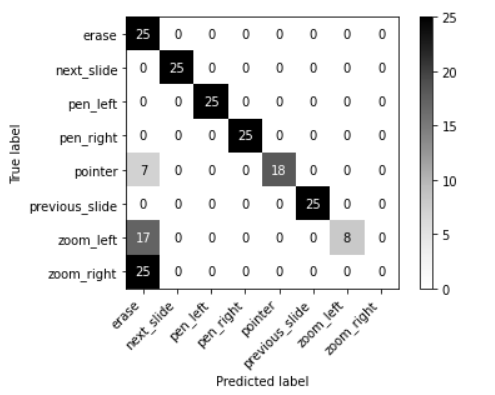
\includegraphics[scale=0.79]{gambar/pengujian-jarak/homogen-dataset/80cm.png}
  \caption{Pengujian Tanpa Variasi Jarak Dataset (80 cm)}
  \label{fig:Pengujian Tanpa Variasi Jarak Dataset (80 cm)}
\end{figure}

\hfill \break
\hfill \break

\begin{figure}[!htb]
  \centering
  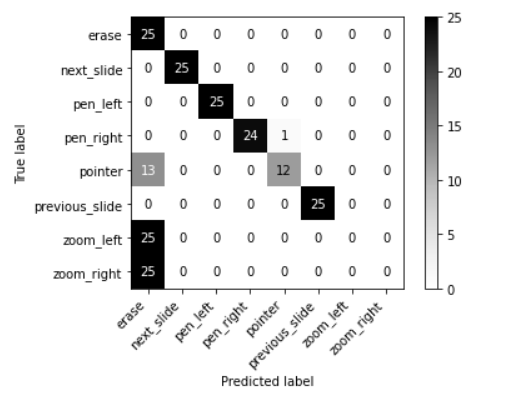
\includegraphics[scale=0.8]{gambar/pengujian-jarak/homogen-dataset/100cm.png}
  \caption{Pengujian Tanpa Variasi Jarak Dataset (100 cm)}
  \label{fig:Pengujian Tanpa Variasi Jarak Dataset (100 cm)}
\end{figure}

\begin{longtable}{|c|c|c|c|c|}
  \caption{Hasil Pengujian Tanpa Variasi Jarak Dataset}
  \label{tb:Hasil Pengujian Tanpa Variasi Jarak Dataset}\\
  \hline
  \rowcolor[HTML]{FFFFFF}
  \textbf{No.} & \textbf{Jarak} & \textbf{Data Terdeteksi Benar} & \textbf{Data Terdeteksi Salah} & \textbf{Akurasi(\%)} \\
  \hline
  1 & 40 cm  & 192 & 8 & 96.00\%  \\
  2 & 60 cm  & 190 & 10 & 95.00\%  \\
  3 & 80 cm  & 151 & 49 & 75.50\%  \\
  4 & 100 cm & 136 & 64 & 68.00\%  \\
  \hline
\end{longtable}

\subsubsection{Pengujian Menggunakan Dataset dengan Jarak Bervariasi}
\label{subsubsec:Pengujian Menggunakan Dataset dengan Jarak Bervariasi}
Dalam pengujian ini, model yang digunakan memiliki dataset yang jaraknya beda-beda. Penulis mengambil dataset tiap kelasnya dengan cara bergerak mulai dari jarak sekitar 40 cm terhadap kamera, dan perlahan-lahan mundur sampai jarak sekitar 100 cm. Hasil distribusi tiap kelasnya dapat dilihat pada Gambar \ref{fig:Pengujian Dataset dengan Variasi Jarak (40 cm)}, \ref{fig:Pengujian Dataset dengan Variasi Jarak (60 cm)}, \ref{fig:Pengujian Dataset dengan Variasi Jarak (60 cm)}, dan \ref{fig:Pengujian Dataset dengan Variasi Jarak (100 cm)}. Persebaran prediksi klasifikasinya lebih stabil dan umumnya berada pada kelas yang benar apabila dibandingkan dengan dataset tanpa variasi jarak. 

Dalam pengujian dengan jarak dataset yang bervariasi ini didapatkan ringkasan hasil data seperti pada Tabel \ref{tb:Hasil Pengujian Dataset dengan Variasi Jarak}. Berdasarkan data tersebut didapatkan hasil bahwa tingkat akurasi memang mengalami penurunan setiap jaraknya diperlebar. Namun, akurasi yang dihasilkan masih tetap lebih tinggi dibanding model sebelumnya. 

Saat jarak 40 cm didapatkan akurasi sebesar 99.00\%, saat jarak 60 cm didapatkan akurasi 97.50\%, Kemudian saat jarak 80 cm akurasinya sebesar 97.00\%, dan saat jarak 100 cm didapatkan akurasi sebesar 94.50\%. Dari data ini dapat diketahui bahwa variasi jarak pada dataset sangat mempengaruhi akurasi apabila pengambilan data citra dilakukan dengan jarak yang bervariasi juga.

\begin{figure}[!htb]
  \centering
  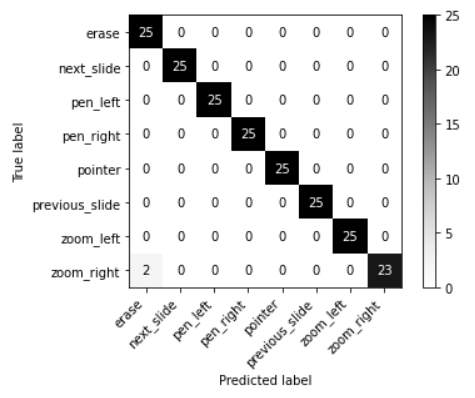
\includegraphics[scale=0.78]{gambar/pengujian-jarak/heterogen-dataset/40cm.png}
  \caption{Pengujian Dataset dengan Variasi Jarak (40 cm)}
  \label{fig:Pengujian Dataset dengan Variasi Jarak (40 cm)}
\end{figure}

\begin{figure}[!htb]
  \centering
  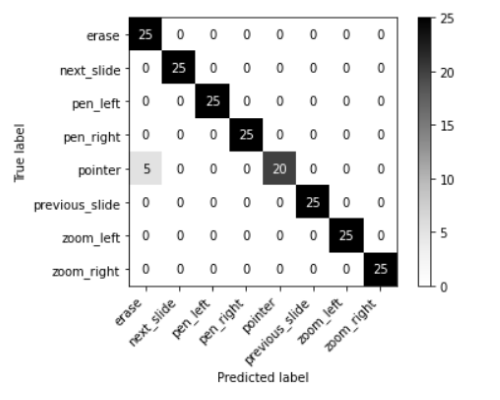
\includegraphics[scale=0.78]{gambar/pengujian-jarak/heterogen-dataset/60cm.png}
  \caption{Pengujian Dataset dengan Variasi Jarak (60 cm)}
  \label{fig:Pengujian Dataset dengan Variasi Jarak (60 cm)}
\end{figure}

\begin{figure}[!htb]
  \centering
  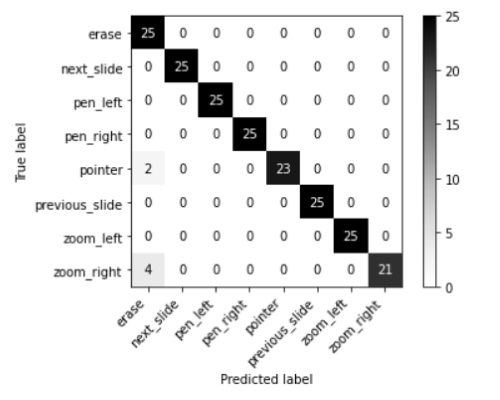
\includegraphics[scale=0.78]{gambar/pengujian-jarak/heterogen-dataset/80cm.png}
  \caption{Pengujian Dataset dengan Variasi Jarak (80 cm)}
  \label{fig:Pengujian Dataset dengan Variasi Jarak (80 cm)}
\end{figure}

\hfill \break
\hfill \break
\hfill \break
\hfill \break

\begin{figure}[!htb]
  \centering
  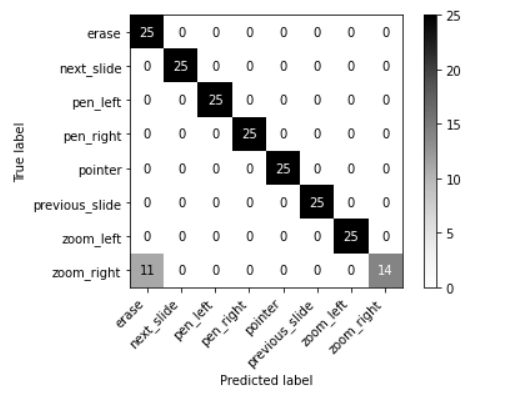
\includegraphics[scale=0.8]{gambar/pengujian-jarak/heterogen-dataset/100cm.png}
  \caption{Pengujian Dataset dengan Variasi Jarak (100 cm)}
  \label{fig:Pengujian Dataset dengan Variasi Jarak (100 cm)}
\end{figure}

\begin{longtable}{|c|c|c|c|c|}
  \caption{Hasil Pengujian Dataset dengan Variasi Jarak}
  \label{tb:Hasil Pengujian Dataset dengan Variasi Jarak}\\
  \hline
  \rowcolor[HTML]{FFFFFF}
  \textbf{No.} & \textbf{Jarak} & \textbf{Data Terdeteksi Benar} & \textbf{Data Terdeteksi Salah} & \textbf{Akurasi(\%)} \\
  \hline
  1 & 40 cm  & 198 & 2 & 99.00\%  \\
  2 & 60 cm  & 195 & 5 & 97.50\%  \\
  3 & 80 cm  & 194 & 6 & 97.00\%  \\
  4 & 100 cm & 189 & 11 & 94.50\%  \\
  \hline
\end{longtable}

\subsection{Hasil Pengujian Menggunakan Variasi Pencahayaan}
\label{subsec:Hasil Pengujian Menggunakan Variasi Pencahayaan}

\begin{figure}[!htb]
  \centering
  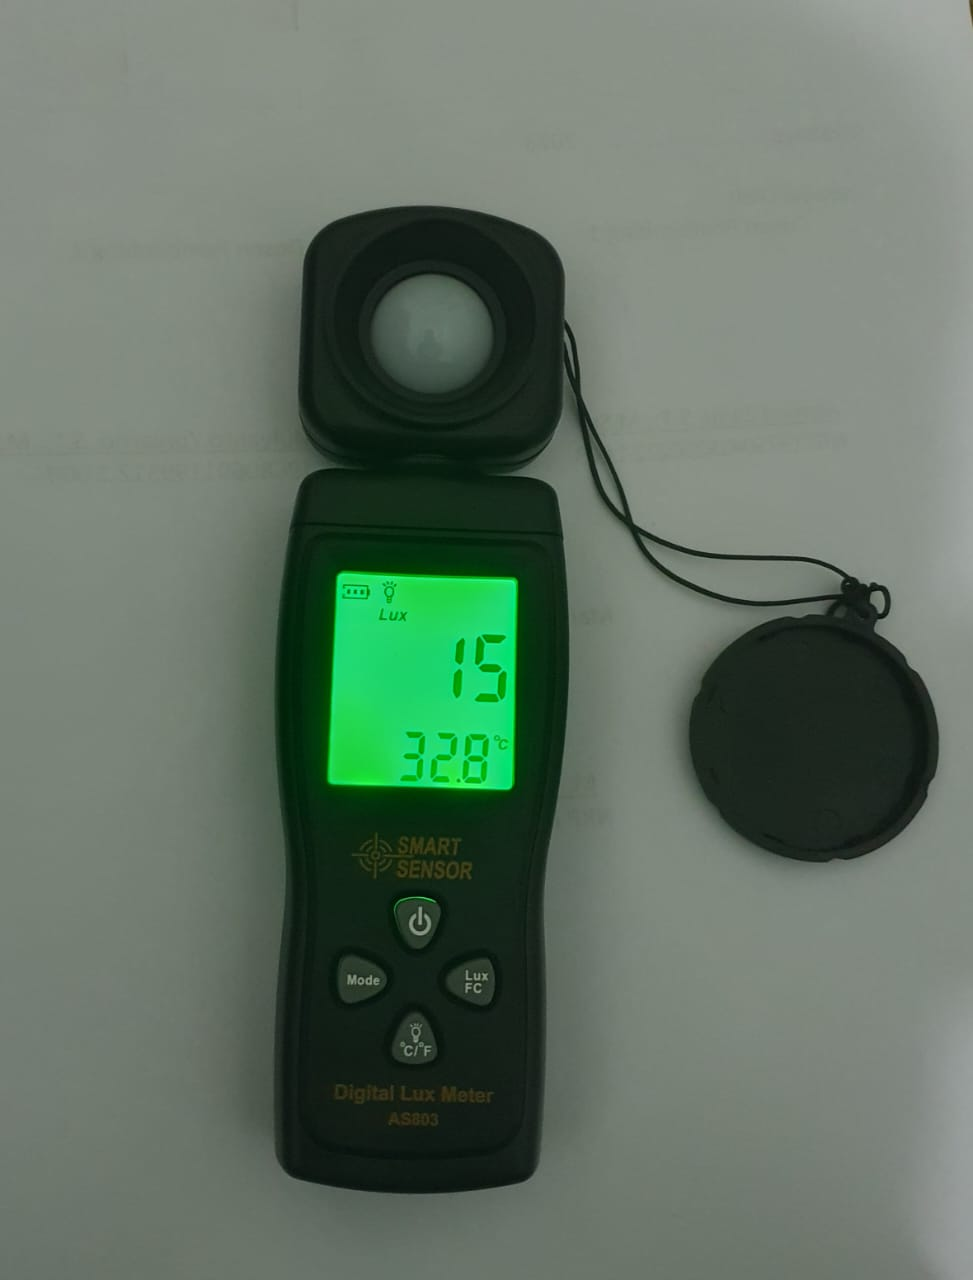
\includegraphics[scale=0.15]{gambar/lux-meter.jpeg}
  \caption{\emph{Digital Lux Meter}}
  \label{fig:Digital Lux Meter}
\end{figure}

Pengujian menggunakan variasi Pencahayaan yang berbeda-beda ini dilakukan dengan tujuan untuk menguji performa tingkat keterbacaan pose tangan dalam berbagai kondisi cahaya di tempat pengambilan citra. Dalam mengukur pencahayaan ini sendiri digunakan alat ukur bernama \emph{Digital Lux Meter}, yang dapat dilihat pada Gambar \ref{fig:Digital Lux Meter}. \emph{Lux Meter} merupakan perangkat yang mengukur banyaknya cahaya masuk menggunakan satuan lux dalam perhitungannya. Satuan lux sendiri adalah besarnya arus cahaya yang datang persatuan luas permukaan. Sehingga, alat ini dapat menjadi acuan tiap kondisi pencahayaan dalam skenario pengujian kali ini.

Variasi pencahayaannya dibagi menjadi tiga kondisi. Kondisi pertama adalah didalam ruangan yang mendapat cahaya lampu dengan cerah. Jika diukur dengan \emph{lux meter} nilainya pada kisaran 40 lx. Kondisi kedua adalah pencahayaan yang redup, dimana pengujian diambil tetap dalam ruangan namun kondisi lampu mati dan hanya memanfaatkan cahaya matahari dari celah-celah jendela dan pintu ruangan. Apabila diukur dengan \emph{lux meter} didapatkan angka sebesar 15 lx. Kondisi terakhir adalah kondisi pencahayaan gelap, dimana pengujian dilakukan dalam ruangan tanpa cahaya lampu dan matahari. Sumber cahaya yang ada hanya dari layar laptop. Dalam kondisi ketiga ini didapatkan angka pada \emph{lux meter} sebesar 5 lx. Gambaran kondisi pengambilan data pengujian untuk kondisi terang dapat dilihat pada gambar \ref{fig:kondisi_40lux}, kondisi redup pada gambar \ref{fig:kondisi_15lux}, dan kondisi gelap pada gambar \ref{fig:kondisi_5lux}.

\begin{figure}[!htb]
  \centering
  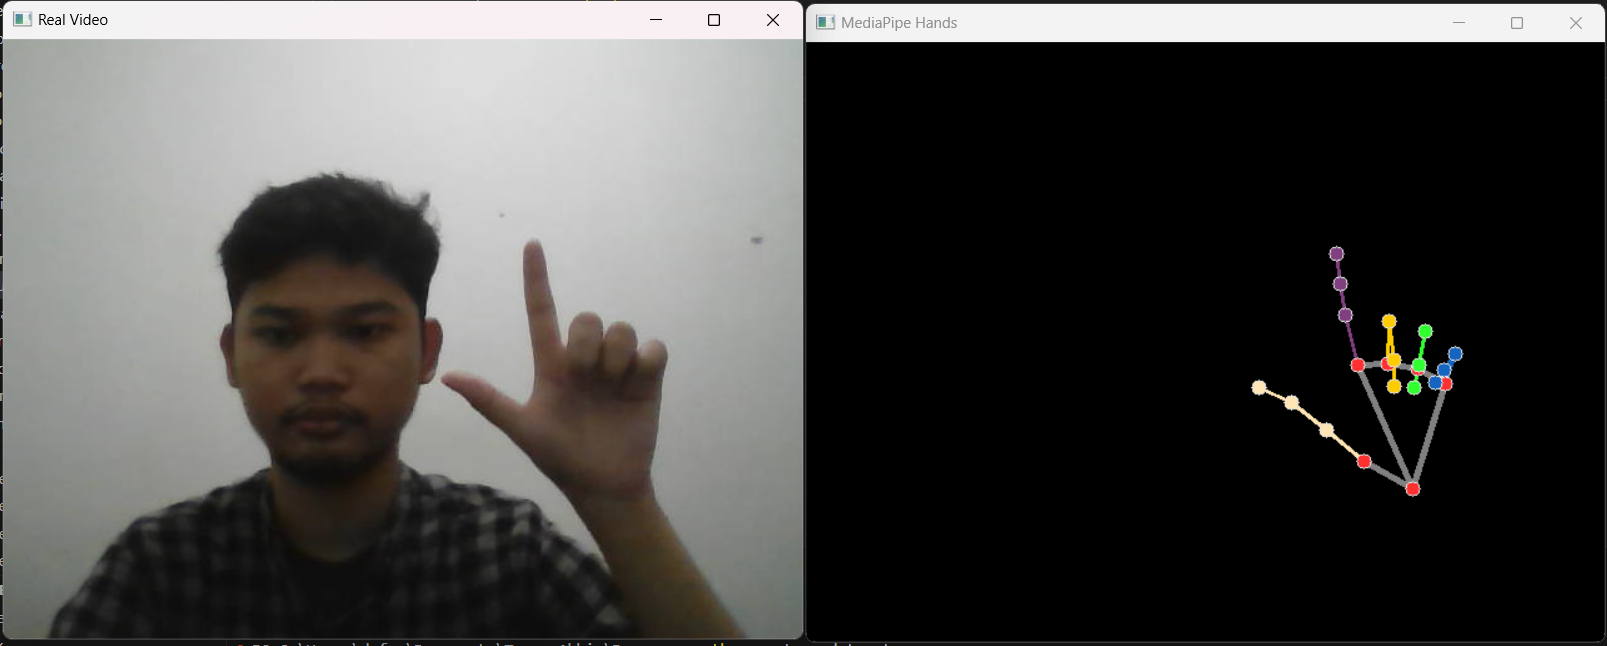
\includegraphics[scale=0.4]{gambar/pengujian-cahaya/kondisi_40lux.png}
  \caption{Kondisi Terang(40 lx)}
  \label{fig:kondisi_40lux} 
\end{figure}

\begin{figure}[!htb]
  \centering
  \includegraphics[scale=0.4]{gambar/pengujian-cahaya/kondisi_15lux.png}
  \caption{Kondisi Terang(15 lx)}
  \label{fig:kondisi_15lux} 
\end{figure}

\hfill \break

\begin{figure}[!htb]
  \centering
  \includegraphics[scale=0.4]{gambar/pengujian-cahaya/kondisi_5lux.png}
  \caption{Kondisi Terang(5 lx)}
  \label{fig:kondisi_5lux} 
\end{figure}

Persebaran hasil klasifikasi yang benar dan salah untuk pencahayaan kondisi gelap ada pada Gambar \ref{fig:Pengujian Dataset dengan Variasi Pencahayaan 5lux}. Hasil klasifikasi dimana citra yang sebenarnya termasuk klasifikasi \emph{'pointer'} tapi salah terdeteksi kedalam \emph{'erase'}. Hal ini bisa terjadi karena dikondisi gelap terkadang ada bagian yang terjadi kesalahan prediksi. Pada citra \emph{'pointer'} misalnya, bagian jari kelingking dan jempol yang tidak terdeteksi. Sehingga, pose pointer jadi terlihat seperti pose \emph{'erase'}. Hal inilah yang menyebabkan terdapat 14 citra \emph{'pointer'} yang salah terdeteksi kedalam kelas \emph{'erase'}. 

Berdasarkan pengujian yang dilakukan, didapatkan data seperti yang tertera dalam tabel \ref{tb:Hasil Pengujian dengan Variasi Pencahayaan}. Dalam data tersebut menunjukkan bahwa dalam kondisi cahaya terang, tingkat akurasi yang dicapai sebesar 99.00\%. Sedangkan untuk kondisi cahaya redup akurasinya yang didapatkan sebesar 96.00\%. Terakhir, dalam kondisi pencahayaan gelap akurasinya sebesar 89.00\%. Melalui data tersebut memang terjadi penurunan akurasi saat setiap kondisi pencahayaan semakin menurun. 

Namun, penurunan akurasi yang terjadi tidak terlalu signifikan, bahkan sampai dalam kondisi pencahayaan sangat gelap sekalipun. Hal ini lebih banyak dipengaruhi faktor kemampuan dalam \emph{library mediapipe}. Selama \emph{mediapipe} masih dapat mendeteksi \emph{landmark} tangan dengan tepat, maka model klasifikasi pun juga tetap mampu memprediksi pose dengan tepat juga. Karena, yang dibaca oleh model adalah \emph{landmark} tangan yang sudah diproses \emph{mediapipe}, bukan gambar pose tangan langsung dari kamera. 

\begin{figure}[!htb]
  \centering
  \includegraphics[scale=0.7]{gambar/pengujian-cahaya/40lux.png}
  \caption{Pengujian Dataset dengan Variasi Pencahayaan (40 lx)}
  \label{fig:Pengujian Dataset dengan Variasi Pencahayaan 40lux} 
\end{figure}

\begin{figure}[!htb]
  \centering
  \includegraphics[scale=0.75]{gambar/pengujian-cahaya/15lux.png}
  \caption{Pengujian Dataset dengan Variasi Pencahayaan (15 lx)}
  \label{fig:Pengujian Dataset dengan Variasi Pencahayaan 15lux} 
\end{figure}

\begin{figure}[!htb]
  \centering
  \includegraphics[scale=0.75]{gambar/pengujian-cahaya/5lux.png}
  \caption{Pengujian Dataset dengan Variasi Pencahayaan (5 lx)}
  \label{fig:Pengujian Dataset dengan Variasi Pencahayaan 5lux} 
\end{figure}

\begin{longtable}{|c|c|c|c|c|}
  \caption{Hasil Pengujian dengan Variasi Pencahayaan}
  \label{tb:Hasil Pengujian dengan Variasi Pencahayaan}\\
  \hline
  \rowcolor[HTML]{FFFFFF}
  \textbf{No.} & \textbf{Cahaya} & \textbf{Data Terdeteksi Benar} & \textbf{Data Terdeteksi Salah} & \textbf{Akurasi(\%)} \\
  \hline
  1 & Terang (40 lx)  & 198 & 2 & 99.00\%  \\
  2 & Redup (15 lx)   & 192 & 8 & 96.00\%  \\
  3 & Gelap (5 lx)    & 178 & 22 & 89.00\%  \\
  \hline
\end{longtable}

\subsection{Hasil Pengujian \emph{Frame Rate}}
\label{subsec:Hasil Pengujian Frame Rate}

\emph{Frame Rate} pada umumnya dinyatakan dalam satuan per detik atau disebut sebagai \emph{Frame Per Second (FPS)}. FPS ini merupakan pengukuran seberapa banyak jumlah frame yang ada dalam satu detik. Pengujian \emph{Frame Rate} dianggap penting karena menjadi salah satu penilaian performa dari model yang dibuat. Selain itu, \emph{Frame Rate} juga sangat mempengaruhi penilaian \emph{user experience}. Apabila semakin kecil nilainya maka gerakan semakin terlihat patah-patah, dan respon yang diberikan semakin lambat. Sebaliknya, semakin besar nilainya maka  gerakan yang dihasilkan lebih lancar dan responnya semakin cepat.

\newpage

\begin{figure}[!htb]
  \centering
  \includegraphics[scale=0.7]{gambar/pengujian-fps/grafik-pengujian-fps.png}
  \caption{Grafik Pengujian \emph{Frame Rate}}
  \label{fig:Grafik Pengujian Frame Rate}
\end{figure}

Pada pengujian kali ini, perhitungan \emph{frame rate} diuji dengan mengambil data nilai FPS setiap detiknya selama 30 detik pada kondisi ideal yaitu cahaya terang dan jarak sekitar 40 cm - 60 cm. Hasil pengujian \emph{frame rate} dapat dilihat pada gambar \ref{fig:Grafik Pengujian Frame Rate}. Berdasarkan grafik pada Gambar \ref{fig:Grafik Pengujian Frame Rate}, didapatkan nilai rata-rata FPS yang didapatkan sebesar 20.86 FPS, dengan rincian nilai tertingginya bisa mencapai 25 FPS, dan titik terendahnya mendekati 15 FPS. Berdasarkan data ini dapat dinyatakan bahwa performa model memungkinkan untuk masih dapat mendeteksi pose tangan dengan baik. 

\subsection{Hasil Pengujian dari Responden yang Berbeda}
\label{subsec:Hasil Pengujian dari Responden yang Berbeda}
Saat pengambilan dataset untuk proses \emph{training} model, data yang digunakan hanya menggunakan pose tangan penulis saja. Sehingga, perlu dilakukan pengujian apabila pose tangan yang dideteksi merupakan tangan selain penulis yang mungkin secara ukuran berbeda. Hal ini bertujuan untuk mengetahui tingkat akurasi model apabila tangan yang dideteksi memiliki ukuran atau bentuk yang tidak sama dengan tangan penulis yang dijadikan dataset.

Dalam pengujian ini, kondisi pengambilan data responden dilakukan dikondisi ideal. Kondisi ideal yang dimaksud disini adalah kondisi dengan tingkat akurasi paling tinggi yang sudah diuji dalam skenario pengujian pada subbab \ref{subsec:Hasil Pengujian Menggunakan Variasi Jarak} dan \ref{subsec:Hasil Pengujian Menggunakan Variasi Pencahayaan}. Berdasarkan data tersebut, didapatkan bahwa kondisi paling ideal adalah saat jarak tangan dengan kamera diangka 40 cm. Sedangkan, untuk kondisi cahayanya dilakukan didalam ruangan yang terang (sekitar 40 lx). Berikut ini adalah hasil pengujiannya.

\subsubsection{Pengujian Menggunakan Data Citra dari Responden 1}
\label{subsec:Pengujian Menggunakan Data Citra dari Responden 1}

Pada saat pengambilan data citra, responden 1 diposisikan untuk berada pada kondisi dengan tingkat akurasi paling ideal, dan diambil data citra sebanyak 25 frame pada tiap kelasnya, yang berarti total data citra yang diambil sebanyak 200 data. Berdasarkan gambar \ref{fig:Pengujian Menggunakan Data Citra dari Responden 1} didapatkan tingkat akurasi yang dihasilkan sebesar 88.00\%. Hal ini berarti menunjukkan adanya penurunan akurasi dari model dengan input citra dari penulis. Namun, penurunan yang terjadi tidak terlalu jauh, sehingga masih input citra masih dapat terdeteksi dengan akurasi cukup baik. 

\begin{figure}[!htb]
  \centering
  \includegraphics[scale=0.5]{gambar/pengujian-ukuran-tangan/tangan-alfan.png}
  \caption{Pengujian Menggunakan Data Citra dari Responden 1}
  \label{fig:Pengujian Menggunakan Data Citra dari Responden 1}
\end{figure}

\subsubsection{Pengujian Menggunakan Data Citra dari Responden 2}
\label{subsec:Pengujian Menggunakan Data Citra dari Responden 2}

Kondisi pengambilan data citra untuk responden 2, sama dengan responden satu yaitu diposisikan untuk berada pada kondisi dengan tingkat akurasi paling ideal. Jumlah data citra yang diambil juga sebanyak 25 frame pada tiap kelasnya, sehingga total data citranya sebanyak 200 data. Hasilnya dapat dilihat pada gambar \ref{fig:Pengujian Menggunakan Data Citra dari Responden 2}. Didapatkan tingkat akurasi yang dihasilkan sebesar 99.50\%. Hal ini berarti menunjukkan adanya penurunan akurasi dari model dengan input citra dari penulis. Namun, penurunan yang terjadi tidak terlalu jauh, dan bahkan lebih baik dibandingkan dengan responden 1. 

\begin{figure}[ht]
  \centering
  \includegraphics[scale=0.85]{gambar/pengujian-ukuran-tangan/tangan-ari.png}
  \caption{Pengujian Menggunakan Data Citra dari Responden 2}
  \label{fig:Pengujian Menggunakan Data Citra dari Responden 2}
\end{figure}

\subsubsection{Pengujian Menggunakan Data Citra dari Responden 3}
\label{subsec:Pengujian Menggunakan Data Citra dari Responden 3}

Pengambilan data pengujian dilakukan sebanyak 25 citra tiap kelasnya yang diambil pada kondisi ideal. Hasilnya dapat dilihat pada gambar \ref{fig:Pengujian Menggunakan Data Citra dari Responden 3}. Didapatkan tingkat akurasi yang dihasilkan sebesar 86,50\%. Sama dengan responden 1 terdapat adanya penurunan akurasi dari model dengan input citra dari penulis, walaupun masih lebih besar dari 80\%. 

\begin{figure}[ht]
  \centering
  \includegraphics[scale=0.5]{gambar/pengujian-ukuran-tangan/tangan-meril.png}
  \caption{Pengujian Menggunakan Data Citra dari Responden 3}
  \label{fig:Pengujian Menggunakan Data Citra dari Responden 3}
\end{figure}

\subsubsection{Pengujian Menggunakan Data Citra dari Responden 4}
\label{subsec:Pengujian Menggunakan Data Citra dari Responden 4}

Proses pengambilan data citra sama dengan responden sebelumnya, yang dilakukan pada kondisi dengan tingkat akurasi paling ideal. Jumlah data yang digunakan juga sama persis. Hasilnya dapat dilihat pada gambar \ref{fig:Pengujian Menggunakan Data Citra dari Responden 4}. Didapatkan tingkat akurasi yang dihasilkan sebesar 89,50\%. Hal ini berarti menunjukkan adanya penurunan akurasi dari model dengan input citra dari penulis, walaupun akurasinya masih mendekati 90\%.

\begin{figure}[ht]
  \centering
  \includegraphics[scale=0.5]{gambar/pengujian-ukuran-tangan/tangan-bakar.png}
  \caption{Pengujian Menggunakan Data Citra dari Responden 4}
  \label{fig:Pengujian Menggunakan Data Citra dari Responden 4}
\end{figure}

Berdasarakan data dari keempat responden yang diambil, dapat diambil ringkasan seperti yang terlihat pada tabel \ref{tb:Hasil Pengujian dengan Variasi Ukuran Tangan}. Memang terjadi adanya penurunan akurasi apabila dibandingkan antara tangan penulis dengan menggunakan tangan responden. Namun, penurunan yang terjadi tidak signifikan, dimana saat menggunakan tangan penulis akurasi yang didapatkan sebesar 98.00\%, sedangkan saat menggunakan tangan responden lain didapatkan rata-rata akurasi sebesar 90.00\%. 

\begin{longtable}{|c|c|c|c|c|}
  \caption{Hasil Pengujian dengan Variasi Ukuran Tangan}
  \label{tb:Hasil Pengujian dengan Variasi Ukuran Tangan}\\
  \hline
  \rowcolor[HTML]{FFFFFF}
  \textbf{No.} & \textbf{Responden} & \textbf{Data Terdeteksi Benar} & \textbf{Data Terdeteksi Salah} & \textbf{Akurasi(\%)} \\
  \hline
  1 & Responden 1  & 179 & 21 & 88,00  \\
  2 & Responden 2  & 168 & 32 & 99,50  \\
  3 & Responden 3  & 190 & 10 & 86,50  \\
  4 & Responden 4  & 190 & 10 & 89,50  \\
  \hline
\end{longtable}

\subsection{Pengujian Menggunakan Model CNN yang Berbeda}
Pengujian ini bertujuan untuk menguji performa apabila menggunakan model yang lain. Terdapat tiga model yang digunakan yaitu Resnet50, VGG16, dan MobileNet. Pengujian ini dilakukan dengan menguji semua variasi yang sama dengan model yang penulis buat sendiri. Berikut adalah hasil pengujian tiap modelnya.

\subsection{Pengujian Menggunakan Model Resnet50}
\label{subsec:Pengujian Menggunakan Model Resnet50}

Pada pengujian pertama, model yang digunakan untuk diuji performanya adalah ResNet50. Model ResNet diusulkan dengan penggunaan metode bernama \emph{Deep Residual Learning for Image Recognition} oleh Kaiming He, Xiangyu Zhang, Shaoqing Ren dan Jian Sun. Model ini memiliki jumlah layer yang jauh lebih banyak dibandingkan model yang dibuat penulis, yaitu berjumlah 50 layer \parencite{Kaiming2015}. Hasil pengujiannya dapat dilihat pada Tabel \ref{tb:Hasil Pengujian Menggunakan model ResNet50}.

\newcolumntype{M}[1]{>{\centering\arraybackslash}m{#1}}

\begin{longtable}[!htb]{|M{25mm}|M{30mm}|M{30mm}|M{30mm}|c|}
  \caption{Hasil Pengujian Menggunakan model ResNet50}
  \label{tb:Hasil Pengujian Menggunakan model ResNet50}\\
  \hline
  \endhead
    Variasi Pengujian & Total Data untuk testing & Data Terprediksi Benar & Data Terprediksi Salah & Akurasi(\%) \\ \hline
    Pengujian Jarak 40 cm & 200 & 195 & 5 & 97.5 \\ \hline
    Pengujian Jarak 60 cm & 200 & 190 & 10 & 95 \\ \hline
    Pengujian Jarak 80 cm & 200 & 195 & 5 & 97.5 \\ \hline
    Pengujian Jarak 100 cm & 200 & 190 & 10 & 95 \\ \hline
    Pengujian Cahaya Terang & 200 & 189 & 11 & 97.5 \\ \hline
    Pengujian \newline Cahaya Redup & 200 & 190 & 10 & 95 \\ \hline
    Pengujian Cahaya Gelap & 200 & 195 & 5 & 94.5 \\ \hline
    Pengujian Menggunakan Tangan Responden 1 & 200 & 183 & 17 & 91.5 \\ \hline
    Pengujian Menggunakan Tangan Responden 2 & 200 & 174 & 26 & 87 \\ \hline
    Pengujian Menggunakan Tangan Responden 3 & 200 & 187 & 13 & 93.5 \\ \hline
    Pengujian Menggunakan Tangan Responden 4 & 200 & 186 & 14 & 93 \\ \hline
\end{longtable}

Berdasarkan Tabel \ref{tb:Hasil Pengujian Menggunakan model ResNet50}, dalam pengujian jarak mendapatkan hasil akurasi rata-rata sebesar 96,25\%, dimana akurasi tertingginya ada pada angka 97,5\% dan terendahnya 95\%. Hasil ini tidak jauh dibandingkan dengan model yang penulis buat yang tercantum dalam Tabel \ref{tb:Hasil Pengujian Dataset dengan Variasi Jarak}, dimana rata-rata yang didapatkan sebesar 97.5\%.

Sedangkan, untuk pengujian cahaya akurasi sama dengan model yang penulis buat yang dimana akurasinya mengalami penurunan seiring dengan kurangnya cahaya yang masuk. Namun untuk kondisi yang sangat gelap, akurasinya terhitung lebih baik dibandingkan model yang dibuat penulis dimana akurasinya sebesar 94.5\% dibandingkan dengan 89.00\%.

Jenis pengujian yang terakhir adalah menggunakan tangan responden yang berbeda-beda. Akurasi yang dihasilkan lebih besar dari model yang penulis buat. Rata-rata yang didapatkan model ini adalah sebesar 91,25\% dibandingkan dengan 90.00\%.

\begin{figure}[!htb]
  \centering
  \includegraphics[scale=0.74]{gambar/pengujian-fps/grafik-pengujian-fps-resnet.png}
  \caption{Grafik Pengujian \emph{Frame Rate} Model Resnet50}
  \label{fig:Grafik Pengujian Frame Rate Model Resnet50}
\end{figure}

Selain pengujian yang disebutkan pada Tabel \ref{tb:Hasil Pengujian Menggunakan model ResNet50}, terdapat pengujian \emph{frame rate} untuk mengukur performa model dalam memprediksi citra. Hasilnya terdapat pada Gambar \ref{fig:Grafik Pengujian Frame Rate Model Resnet50}, dimana rata-rata nilai FPS-nya berada pada angka 11.66 FPS. Hasil ini lebih kecil dibandingkan dengan model yang dibuat penulis dimana FPS yang didapatkan sebesar 20.86 FPS. 

Berdasarkan analisa diatas bisa disimpulkan bahwa akurasi yang dihasilkan model \emph{ResNet-50} jika dibandingkan dengan model yang penulis buat dan diuji di kondisi ideal hasilnya masih lebih kecil walaupun jaraknya tidak jauh, yaitu 97.5\% dibanding 98.00\%. Namun, untuk performa \emph{frame rate} model ini tergolong cukup rendah diangka 11.66 FPS. 

\subsection{Pengujian Menggunakan Model VGG 16}
\label{subsec:Pengujian Menggunakan Model VGG 16}

VGG16 merupakan arsitektur Convolutional Neural Network (CNN) yang digunakan untuk memenangkan kompetisi ILSVR (Imagenet) 2014. Model ini dianggap sebagai salah satu arsitektur model untuk visi komputer terbaik hingga saat ini. Angka 16 dalam nama model ini mengartikan bahwa model ini memiliki 16 lapisan pembobot. Hal yang menjadi kelebihan tentang VGG16 adalah penggunaan hyperparameter yang tidak banyak. Mereka fokus menggunakan lapisan konvolusi filter 3x3 pada langkah 1, dan selalu menggunakan padding yang sama dan lapisan filter maxpool 2x2 pada langkah 2. Ini mengikuti pengaturan ini agar konsisten di seluruh lapisan arsitektur convolutional dan max pooling. Pada akhir layernya sendiri memiliki 2 Fully-Connected layer diikuti oleh softmax untuk output.

\begin{longtable}[!htb]{|M{25mm}|M{30mm}|M{30mm}|M{30mm}|c|}
  \caption{Hasil Pengujian Menggunakan model VGG 16}
  \label{tb:Hasil Pengujian Menggunakan model VGG 16}\\
  \hline
  \textbf{Variasi Pengujian} & \textbf{Total Data untuk testing} & \textbf{Data Terprediksi Benar} & \textbf{Data Terprediksi Salah} & \textbf{Akurasi(\%)} \\ 
  \hline
  \endhead
  Pengujian Jarak 40 cm & 200 & 178 & 22 & 89 \\ \hline
  Pengujian Jarak 60 cm & 200 & 193 & 7 & 96.5 \\ \hline
  Pengujian Jarak 80 cm & 200 & 193 & 7 & 96.5 \\ \hline
  Pengujian Jarak 100 cm & 200 & 199 & 1 & 99.5 \\ \hline
  Pengujian Cahaya Terang & 200 & 176 & 24 & 89 \\ \hline
  Pengujian Cahaya Redup & 200 & 179 & 21 & 89.5 \\ \hline
  Pengujian Cahaya Gelap & 200 & 178 & 22 & 88 \\ \hline
  Pengujian Menggunakan Tangan Responden 1 & 200 & 167 & 33 & 83.5 \\ \hline
  Pengujian Menggunakan Tangan Responden 2 & 200 & 176 & 24 & 88 \\ \hline
  Pengujian Menggunakan Tangan Responden 3 & 200 & 135 & 65 & 67.5 \\ \hline
  Pengujian Menggunakan Tangan Responden 4 & 200 & 184 & 16 & 92 \\ \hline
\end{longtable}

Data dalam tabel \ref{tb:Hasil Pengujian Menggunakan model VGG 16}, menunjukkan bahwa dalam pengujian jarak, akurasi malah turun saat jarak menjadi semakin dekat. Sebagai contoh, ketika jarak 100 cm akurasinya sebesar 96.5\%, namun ketika jarak 40 cm akurasinya menjadi 89\%. Walaupun rata-rata akurasinya masih diangka 94,62 \%. Namun, akurasinya lebih kecil dibandingkan dengan model yang penulis buat yang ada diangka 97.5\%.

Pada pengujian cahaya, akurasinya juga lebih kecil dibanding model yang dibuat penulis. Akurasi model pada pengujian cahaya ini dikondisi terangnya ada pada angka 89\%, sedangkan model yang penulis buat ketika kondisi terangnya ada pada 98\%. Walaupun pada kondisi yang benar-benar gelap akurasi yang dihasilkan tidak jauh beda diangka sekitar 88\%.

Dalam pengujian menggunakan tangan dari beberapa responden, hasil tingkat akurasi yang didapatkan kurang stabil atau konsisten. Sebagai contoh, pada responden ke-4 akurasi yang dihasilkan sebesar 92\%. Namun, begitu diterapkan pada tangan dari responden ke-3, akurasinya turun pada angka 67.5\%.

Penurunan performa model ini juga terjadi pada pengujian \emph{frame rate}. Berdasarkan grafik pada Gambar \ref{fig:Grafik Pengujian Frame Rate Model VGG 16}, didapatkan data bahwa rata-rata FPS yang dihasilkan sebesar 11,96 FPS. Hasil ini lebih kecil dibandingkan model yang dibuat penulis dimana mendapatkan 20,86 FPS.

Melalui analisa diatas, dapa dikatakan bahwa akurasi yang dihasilkan model \emph{VGG 16} angkanya lebih kecil jika dibandingkan dengan model yang penulis buat, terutama pada kondisi saat menggunakan tangan dari responden yang tidak ada pada dataset. Performa \emph{frame rate} juga lebih kecil hasilnya karena hanya dapat memproses sampai 11.96 FPS.
\newpage

\begin{figure}[!htb]
  \centering
  \includegraphics[scale=0.8]{gambar/pengujian-fps/grafik-pengujian-fps-vgg16.png}
  \caption{Grafik Pengujian \emph{Frame Rate} Model VGG 16}
  \label{fig:Grafik Pengujian Frame Rate Model VGG 16}
\end{figure}

\subsection{Pengujian Menggunakan Model MobileNet}
\label{subsec:Pengujian Menggunakan Model MobileNet}

MobileNets merupakan salah satu CNN yang seperti namanya, dapat digunakan pada perangkat mobile. Peneliti dari Google telah menciptakan arsitektur CNN yang dapat mengatasi kebutuhan resource komputasi yang berlebihan. Perbedaan mendasar antara arsitektur MobileNet dengan arsitektur CNN biasanya adalah penggunaan layer atau lapisan konvolusional dengan ketebalan filter yang sesuai dengan ketebalan citra masukan. MobileNet membagi konvolusi menjadi \emph{depthwise convolution} dan \emph{pointwise convolution}.

\begin{longtable}[!htb]{|M{25mm}|M{30mm}|M{30mm}|M{30mm}|c|}
  \caption{Hasil Pengujian Menggunakan Model MobileNet}
  \label{tb:Hasil Pengujian Menggunakan Model MobileNet}\\
  \hline
  \textbf{Variasi Pengujian} & \textbf{Total Data untuk Testing} & \textbf{Data Terprediksi Benar} & \textbf{Data Terprediksi Salah} & \textbf{Akurasi(\%)} \\ 
  \hline
  \endhead
  Pengujian Jarak 40 cm & 200 & 192 & 8 & 96 \\ \hline
  Pengujian Jarak 60 cm & 200 & 200 & 0 & 100 \\ \hline
  Pengujian Jarak 80 cm & 200 & 200 & 0 & 100 \\ \hline
  Pengujian Jarak 100 cm & 200 & 200 & 0 & 100 \\ \hline
  Pengujian Cahaya Terang & 200 & 193 & 7 & 96.5 \\ \hline
  Pengujian Cahaya Redup & 200 & 193 & 7 & 96.5 \\ \hline
  Pengujian Cahaya Gelap & 200 & 192 & 8 & 96 \\ \hline
  Pengujian Menggunakan Tangan Responden 1 & 200 & 199 & 1 & 99.5 \\ \hline
  Pengujian Menggunakan Tangan Responden 2 & 200 & 180 & 20 & 90 \\ \hline
  Pengujian Menggunakan Tangan Responden 3 & 200 & 191 & 9 & 95.5 \\ \hline
  Pengujian Menggunakan Tangan Responden 4 & 200 & 198 & 2 & 99 \\ \hline
\end{longtable}

Pada pengujian jarak, model mobileNet memiliki akurasi paling tinggi dibanding model yang lain. Berdasarkan Tabel \ref{tb:Hasil Pengujian Menggunakan Model MobileNet}, hasil akurasi rata-ratanya sebesar 99\%, dimana akurasi tertingginya ada pada angka 100\% dan terendahnya 96\%. Hasil ini tentu lebih besar dibandingkan dengan model yang penulis buat yang rata-rata akurasi jaraknya sebesar 97.5\%.

Dalam pengujian cahaya, akurasi model ini juga masih menjadi yang tertinggi dibandingkan model yang lain. Model ini dapat memprediksi secara stabil dengan tingkat akurasi selalu berada pada kisaran 96,5\%. Bahkan dalam kondisi paling gelap sekalipun tidak terjadi penurunan yang signifikan. 

Pengujian yang terakhir yaitu menggunakan variasi dari tangan responden, didapatkan hasil yang juga tertinggi diantara model lain. Rata-rata akurasinya diangka 96\%, dengan nilai akurasi paling kecilnya masih diangka 90\%.

\begin{figure}[!htb]
  \centering
  \includegraphics[scale=0.8]{gambar/pengujian-fps/grafik-pengujian-fps-mobilenet.png}
  \caption{Grafik Pengujian \emph{Frame Rate} Model \emph{MobileNet}}
  \label{fig:Grafik Pengujian Frame Rate Model MobileNet}
\end{figure}

Sedangkan, dalam pengujian \emph{frame rate}, model \emph{MobileNet} ini masih lebih tinggi dibandingkan model \emph{Resnet50} maupun \emph{VGG 16}. Dapat dilihat dalam grafik Gambar \ref{fig:Grafik Pengujian Frame Rate Model MobileNet}, rata-rata yang dihasilkan sebesar 17.26 FPS. Namun, FPS dari model ini masih lebih kecil dibandingkan model yang dibuat oleh penulis. Karena memang dari sisi jumlah layer dan hasil akhir ukuran file model jauh lebih kecil. Pada model \emph{MobileNet} ukuran file modelnya sebesar 136 MB. Sedangkan model yang dibuat penulis ukuran filenya hanya sebesar 43 MB saja.

Berdasarkan penyajian data dan analisa ini dapat dikatakan bahwa model \emph{MobileNet} memiliki performa yang paling baik diantara semua model yang diuji pada tugas akhir ini. Tingkat akurasi yang dihasilkan baik pada kondisi yang ideal maupun kurang ideal, model ini masih menghasilkan semua akurasi diangka lebih besar dari 90\% semuanya. FPS yang dihasilkan juga lebih tinggi dibanding model \emph{Resnet50} dan \emph{VGG 16} dengan angka 17,26 FPS.

\subsection{Pengujian \emph{User Experience}}
\label{subsec:Pengujian User Experience} 

Skenario pengujian yang terakhir adalah pengujian \emph{user experience} dimana dalam pengujian ini terdapat beberapa responden yang diminta untuk mencoba program yang dibuat. Mereka kemudian diminta untuk menjawab beberapa pertanyaan mengenai seberapa baik pengalaman penggunaan mereka dalam bentuk kuesioner. Melalui data tersebut dapat menguji apakah program ini dapat lebih baik dibandingkan dengan cara kontrol presentasi lain yang sudah tersedia saat ini.

\subsubsection{Model Kuesioner yang Digunakan}
\label{subsubsec:Model Kuesioner yang Digunakan}
Terdapat beberapa cara dalam menguji \emph{user experience}, Salah satunya dengan \emph{User Experience Questionare} (UEQ). UEQ berisi kuesioner yang mudah serta efisien, dan berguna untuk mengukur \emph{user experience} pada sebuah produk yang interaktif. \emph{User Experience} disini didefinisikan sebagai persepsi dan tanggapan seseorang yang dihasilkan saat suatu produk tersebut digunakan. Dengan demikian, \emph{User Experience} dipandang sebagai konsep yang mencakup semua jenis reaksi emosional, kognitif atau fisik mengenai produk jadi yang konkret atau bahkan hanya produk yang masih diasumsikan pembuatannya. Penilaian penggunaan produk ini dapat dinilai baik saat sebelum, selama dan setelah digunakan \parencite{AndreasHinderks}. 

UEQ mengukur menggunakan kuesioner yang berisi skala dan mencakup kesan komprehensif tentang (\emph{User Experience}). Terdapat enam skala penilaian akhir dalam UEQ, berikut rinciannya.

\begin{enumerate}[nolistsep]
  \item\emph{Attractiveness}. \emph{Attractiveness} atau daya tarik menilai kesan secara keseluruhan dari suatu produk. Penilaian ini mengukur apakah pengguna cenderung menyukai atau tidak menyukai produk yang diuji. Oleh karenanya, produk harus dibuat untuk terlihat menarik, menyenangkan, ramah pengguna dan menyenangkan. 
  \item\emph{Perspicuity}. \emph{Perspicuity} atau kejelasan adalah bagian yang menilai seberapa mudah produk untuk dikenali dan dipelajari cara penggunaannya. Sehingga produk harus dibuat untuk bisa melakukan tugas tertentu dengan cepat, efisien, dan dengan cara yang pragmatis.
  \item\emph{Efficiency}. \emph{Efficiency} merupakan penilaian yang mengukur apakah pengguna bisa menyelesaikan fungsi atau fitur tertentu dengan melalui usaha yang sedikit mungkin. Selain itu, reaksi dari produk apakah dapat bereaksi dengan cepat atau tidak. Karena itu, produk harus sederhana, dan mudah dipelajari.
  \item\emph{Dependability}. \emph{Dependability} atau ketepatan menilai apakah interaksi dengan produk ada dibawah kendali dari pengguna. Penilaian ini berkaitan dengan tingkat keakuratan sehingga interaksi yang dihasilkan sesuai dengan prediksi dari pengguna. Hal ini juga berhubungan dengan tingkat keamanan yang dihasilkan dari produk, karena apabila output yang terjadi tidak sesuai dengan yang diharapkan, dapat menimbulkan kesalahan prediksi yang tidak dapat diantisipasi oleh pengguna . Sehingga, item ini menilai apakah produk dapat diprediksi, aman, dan memenuhi harapan pengguna atau tidak.
  \item\emph{Stimulation}. \emph{Stimulation} adalah bagian penilaian yang dapat memiliki efek rangsangan perasaan positif. Perasaan yang timbul ini bisa perasaan menarik, menyenangkan, memotivasi, ataupun seru saat menggunakan produk. Oleh karena itu, produk harus dirancang sedemikian rupa hingga dapat menimbulkan efek rangsangan perasaan menarik dan menyenangkan.
  \item\emph{Novelty}. \emph{Novelty} atau kebaruan merupakan bagian pengukuran yang menilai seberapakah kreatif dan inovatifnya suatu produk. Apabila suatu produk itu memilki nilai inovasi dan kreatif didalamnya, tentu dapat menimbulkan kesan menarik minat bagi pengguna. Sehingga, produk harus memiliki ide awal yang dirancang secara inovatif dan kreatif, serta menggunakan teknologi yang sesuai dengan perkembangan zaman.
\end{enumerate}

\begin{figure}[!htb]
  \centering
  \includegraphics[scale=1.5]{gambar/pengujian-user-experience/soal-kuesioner.png}
  \caption{Soal Kuesioner}
  \label{fig:Soal Kuesioner}
\end{figure}

Pertanyaan yang ada pada kuesioner ini berjumlah 26 item. Setiap item ini menunjukkan skala satu sampai tujuh, dimana penilaian positifnya ini tergantung pada letak item tiap nomor soalnya. Sebagai contoh, dapat dilihat pada gambar \ref{fig:Soal Kuesioner} dimana pada item nomor satu menyenangkan ada pada sisi kanan. Sehingga, semakin skalanya kearah kanan, maka semakin positif penilaiannya. Namun, pada soal nomor tiga, penilaian kreatif ada pada sisi kiri. Hal ini membuat penilaian positifnya justru ada pada skala yang semakin kecil. 

Tujuan dari dibuatnya pertanyaan seperti ini, agar pengguna yang mengisi kuesioner bisa dapat menilai lebih objektif dan teliti. Apabila penilaian positifnya semuanya ada pada sisi kanan, dikhawatirkan beberapa responden tidak melihat item pada tiap soalnya dan hanya mengisi di sisi yang positif semua atau negatif semua.  

Berdasarkan pertanyaan dalam tiap item kuesioner, dikumpulkan dan dianalisis penilaiannya seperti apa. Dalam penggunaan UEQ, sudah terdapat \emph{tools} yang dapat digunakan untuk menilai output dari pengujian ini. Outputnya berupa diagram yang dengan nilai tertentu dari setiap enam skala penilaian dalam UEQ yaitu daya tarik, kejelasan, efisiensi, ketepatan, stimulasi, dan kebaruan.

\subsubsection{Distribusi Responden}
\label{subsubsec:Distribusi Responden}

Pengambilan data kuesioner dilakuakan pada area kampus, dimana umumnya responden memiliki latar belakang sebagai pelajar atau mahasiswa. Alasan pengambilan responden dengan latar belakang tersebut karena mereka adalah salah satu bagian masyarakat yang paling sering melakukan kegiatan presentasi. Sehingga, sasaran responden dianggap tepat dalam pengujian kali ini. 

Jika dilihat berdasarkan usia, responden yang mengisi kuesioner berada pada rentang usia antara 21 sampai 22 tahun. Sedangkan berdasarkan jenis kelamin didominasi oleh pria dengan rincian 86\% pria dan 14\% wanita seperti yang terlihat pada Gambar \ref{fig:Persebaran Data Gender}  

\begin{figure}[!htb]
  \centering
  \includegraphics[scale=1]{gambar/pengujian-user-experience/persebaran-data-gender.png}
  \caption{Persebaran Data Gender}
  \label{fig:Persebaran Data Gender}
\end{figure}

\subsubsection{Hasil Analisa Kuesioner}
\label{subsubsec:Hasil Analisa Kuesioner}

Berdasarkan pengumpulan kuesioner dari responden yang disebutkan pada \ref{subsubsec:Distribusi Responden}, data dimasukkan kedalam \emph{'tool'} yang disediakan dari metode UEQ. Output yang dihasilkan \emph{'tool'} ini berupa data grafis yang menunjukkan seberapa positif atau negatif evaluasi yang diberikan oleh responden. 

Nilai untuk satu item digambarkan dalam skala antara 1 sampai 3. Nilai antara -0,8 dan 0,8 mewakili evaluasi yang kurang lebih dianggap netral. Sedangkan, nilai lebih dari 0,8 mewakili evaluasi atau penilaian yang positif. Sebaliknya, nilai kurang dari -0,8 mewakili evaluasi atau penilaian negatif. Jadi, apabila hasil penilaian ada pada kisaran skala antara -3 berarti sangat buruk dan +3 berarti sangat baik. 

\emph{Ouput} dari grafis yang pertama adalah terkait dengan rata-rata jawaban responden pada setiap item soal. Seperti yang tertera pada Gambar \ref{fig:Jawaban Rata-rata Setiap Item Soal}, rata-rata jawaban dari responden memberikan penilaian yang bersifat positif karena nilainya lebih besar dari 0,8. Terdapat beberapa item penilaian yang dinilai paling positif yaitu item kemudahan untuk dapat dipahami, baiknya program, keamanan saat digunakan, dan kepraktisan penggunaan. 

\begin{figure}[!htb]
  \centering
  \includegraphics[scale=1.15]{gambar/pengujian-user-experience/rata2-tiap-jawaban.png}
  \caption{Jawaban Rata-rata Setiap Item Soal}
  \label{fig:Jawaban Rata-rata Setiap Item Soal}
\end{figure}

Namun, terdapat penilaian yang terhitung bukan positif namun masih ada pada rentang netral. Penilaian itu terkait dengan item daya cipta dan inovasi. Maksud dari item ini adalah terkait dengan seberapa inovatif dan baru ide dari topik tugas akhir ini. Berdasarkan penilaian ini dapat dinyatakan bahwa inovasi dan ide dari tugas akhir ini memang bukan sesuatu yang sangat baru, namun tidak dapat dinyatakan tertinggal juga. 

Berdasarkan semua item soal dalam kuesioner, dapat dikelompokkan menjadi enam penilaian utama yang disebutkan pada \ref{subsubsec:Model Kuesioner yang Digunakan} yaitu \emph{Attractiveness, Perspicuity, Efficiency, Dependability, Stimulation, dan Novelty}. Hasilnya dapat dilihat pada Gambar \ref{fig:Hasil Penilaian User Experience}. 

Pada penilaian pertama terdapat \emph{Attractiveness} atau daya tarik yang mendapatkan poin 1,595. Hal ini menunjukkan bahwa program yang dibuat dapat dinilai terlihat menarik, menyenangkan, serta ramah untuk pengguna yang baru mencoba.

Penilaian yang kedua adalah \emph{Perspicuity} atau kejelasan, dimana didapatkan poin sebesar 1,786. Nilai tersebut menunjukkan bahwa program bisa melakukan tugasnya dengan cepat, efisien, dan dengan cara yang pragmatis.

Penilaian yang ketiga adalah \emph{Efficiency}. Poin yang didapatkan untuk efisiensi sebesar 1,679 yang berarti pengguna bisa menggunakan suatu fungsi atau fitur tertentu dengan melalui usaha yang seminimal mungkin.

Item penilaian yang keempat disebut sebagai\emph{Dependability} atau ketepatan. Didapatkan nilai poin 1,607 yang berarti nilai tersebut menunjukkan bahwa interaksi antara pengguna dengan program yang dijalankan masih ada dibawah kendali dan sesuai dengan perkiraan atau harapan pemakainya.
  
Dalam item penilaian yang kelima ada \emph{Stimulation}. Poin yang didapatkan sebesar 1,714. Hasil penilaian ini menunjukkan bahwa pengguna mendapatkan efek rangsangan perasaan yang positif, baik itu perasaan menarik, menyenangkan, dan seru.

Item Penilaian yang terakhir adalah \emph{Novelty} atau kebaruan. Dalam item penilaian ini didapatkan poin sebesar 0,964. Memang angka ini tidak terhitung cukup tinggi dibandingkan dengan penilaian sebelumnya, namun masih termasuk dalam rentang penilaian positif. Oleh karenanya, program ini masih bisa dikatakan sebagai produk kreatif dan inovatifnya, walaupun memang dinilai oleh beberapa pengguna bukan sebagai suatu ide yang benar-benar baru.

\begin{figure}[!htb]
  \centering
  \includegraphics[scale=1.1]{gambar/pengujian-user-experience/hasil-tiap-penilaian.png}
  \caption{Hasil Penilaian \emph{User Experience}}
  \label{fig:Hasil Penilaian User Experience}
\end{figure}

Berdasarkan analisa pada pengujian \emph{user experience} dapat diambil penilaian bahwa program yang dicoba memberikan pengalaman pengguna dengan hasil reaksi evaluasi yang bersifat positif, terutama dari aspek kemudahan untuk dipahami, kepraktisan dalam penggunaan, dan memberikan pengalaman perasaan menarik dan menyenangkan.
\cleardoublepage

% Bab 5 penutup
\chapter{PENUTUP}
\label{chap:penutup}

% Ubah bagian-bagian berikut dengan isi dari penutup
Dalam bab ini berisi mengenai kesimpulan berdasarkan serangkaian rangkaian pengujian yang dipaparkan dalam Bab \ref{sec:hasilpengujian}, dan disesuaikan dengan tujuan yang berusaha dicapai dalam tugas akhir ini. Pada bab ini juga, terdapat saran-saran yang diberikan dalam rangka meningkatkan dan mengembangkan penelitian selanjutnya yang terkait dengan topik tugas akhir ini. Berikut ini adalah kesimpulan dan saran yang dapat diambil. 

\section{Kesimpulan}
\label{sec:kesimpulan}

Berdasarkan hasil pengujian yang sudah dipaparkan, dapat diambil beberapa kesimpulan sebagai berikut.

\begin{enumerate}[nolistsep]
  \item Klasifikasi citra dengan menggunakan metode Convolutional Neural Network (CNN) dapat digunakan untuk memprediksi citra pose tangan dengan tingkat akurasi mencapai 99.00\%. 
  \item Pada pengujian jarak dapat disimpulkan bahwa variasi pengambilan jarak dataset sangat mempengaruhi akurasi. Dimana, jarak penurunannya akurasinya bisa mencapai 30\%.
  \item Dari hasil pengujian variasi cahaya, disimpulkan bahwa model yang ada tidak mengalami penurunan yang signifikan baik ketika kondisi cahaya terang, redup, bahkan gelap. Penurunan yang terjadi masih dibawah 10\%.
  \item Berdasarkan pengujian \emph{frame rate} dengan menggunakan beberapa model CNN, dapat diambil kesimpulan bahwa kompleksitas dan besar ukuran model sangat mempengaruhi performa FPS-nya. 
  \item Dari hasil klasifikasi model yang didapatkan, dapat dihubungkan dengan berbagai fungsi navigasi ataupun penggunaan beberapa fitur kontrol dalam aplikasi Microsoft PowerPoint. 
  \item Kontrol presentasi menggunakan pose tangan dapat memberikan respon \emph{user experience} positif yang menarik dan mudah digunakan. 
\end{enumerate}   

\section{Saran}
\label{chap:saran}

Dalam rangka pengembangan penelitian kedepan terutama yang terkait dengan topik Convolution Neural Network, pose tangan, ataupun kontrol presentasi, dapat diusulkan beberapa saran yang disebutkan sebagai berikut.

\begin{enumerate}[nolistsep]
  \item Perlu ditambahkan jumlah dataset dengan berbagai variasi jarak pada saat pengambilan dataset. Sehingga diharapkan akurasi hasil klasifikasi tetap baik meskipun diambil dari jarak yang bervariasi.
  \item Menambahkan dataset dengan variasi ukuran tangan dari berbagai macam orang, agar akurasi yang dihasilkan lebih stabil meskipun diuji keresponden yang berbeda-beda.
\end{enumerate} 

\cleardoublepage

\chapter*{DAFTAR PUSTAKA}
\addcontentsline{toc}{chapter}{DAFTAR PUSTAKA}
\renewcommand\refname{}
\vspace{2ex}
\renewcommand{\bibname}{}
\begingroup
\def\chapter*#1{}
\printbibliography
\endgroup
\cleardoublepage

% Biografi penulis
\begin{center}
  \Large
  \textbf{BIOGRAFI PENULIS}
\end{center}

\addcontentsline{toc}{chapter}{BIOGRAFI PENULIS}

\vspace{2ex}

\begin{wrapfigure}{L}{0.3\textwidth}
  \centering
  \vspace{-3ex}
  % Ubah file gambar berikut dengan file foto dari mahasiswa
  \includegraphics[width=0.3\textwidth]{gambar/elon.jpg}
  \vspace{-4ex}
\end{wrapfigure}

% Ubah kalimat berikut dengan biografi dari mahasiswa
\name{}, lahir pada \lipsum[1]

\lipsum[2]

\cleardoublepage

\end{document}
